%%%%%%%%%%%%%%%%%%%%%%%%%%%%%%%%%%%%%%%%%
% Journal Article
% LaTeX Template
% Version 1.4 (15/5/16)
%
% This template has been downloaded from:
% http://www.LaTeXTemplates.com
%
% Original author:
% Frits Wenneker (http://www.howtotex.com) with extensive modifications by
% Vel (vel@LaTeXTemplates.com)
%
% License:
% CC BY-NC-SA 3.0 (http://creativecommons.org/licenses/by-nc-sa/3.0/)
%
%%%%%%%%%%%%%%%%%%%%%%%%%%%%%%%%%%%%%%%%%

%----------------------------------------------------------------------------------------
%	PACKAGES AND OTHER DOCUMENT CONFIGURATIONS
%----------------------------------------------------------------------------------------
\newcommand{\reporttitle}{Risk and Trust in Open Systems}
\newcommand{\reportauthor}{Shu Peng Loh}
\newcommand{\supervisor}{Sophia Drossopoulou}
\newcommand{\degreetype}{Computing Science}
\documentclass[a4paper,11pt,twoside]{article}
\usepackage[usenames,dvipsnames,svgnames,table]{xcolor}
\usepackage[hang,flushmargin]{footmisc} 
\definecolor{light-gray}{gray}{0.95}
\usepackage{listings}
\lstset{
    breaklines=true,
    columns=flexible,
    backgroundcolor=\color{light-gray},
    basicstyle=\sffamily\small,
    escapechar=\&
}
\usepackage[sc]{mathpazo} % Use the Palatino font
\usepackage[T1]{fontenc} % Use 8-bit encoding that has 256 glyphs
\linespread{1.15} % Line spacing - Palatino needs more space between lines
\usepackage{microtype} % Slightly tweak font spacing for aesthetics
\usepackage[english]{babel} % Language hyphenation and typographical rules
\usepackage{multirow}
\usepackage{multicol}
\usepackage[left=2.5cm,right=2.5cm,top=3cm,bottom=3cm, hmarginratio=1:1,headheight=14pt,columnsep=15pt]{geometry} % Document margins
\usepackage[hang, normal,labelfont=bf,up,textfont=sc,up]{caption} % Custom captions under/above floats in tables or figures
\usepackage{booktabs}
\usepackage{pdfpages}
\usepackage{graphicx}
\usepackage{enumitem} % Customized lists
\usepackage{color}
\usepackage{pdfpages}
\setlist[itemize]{noitemsep} % Make itemize lists more compact
\usepackage{ latexsym }
\usepackage{abstract} % Allows abstract customization
\renewcommand{\abstractnamefont}{\normalfont\bfseries} % Set the "Abstract" text to bold
\renewcommand{\abstracttextfont}{\normalfont\small} % Set the abstract itself to small italic text

\usepackage{fancyhdr} % Headers and footers
\fancyhead{} % Blank out the default header
\fancyfoot{} % Blank out the default footer
%\fancyhead[C]{Running title $\bullet$ May 2016 $\bullet$ Vol. XXI, No. 1} % Custom header text
\fancyfoot[RO,LE]{\thepage} % Custom footer text

\usepackage{titling} % Customizing the title section
\usepackage{titlesec}
\titleformat{name=\section}{\flushleft\bf\scshape\Large}{\thesection}{.5em}{}
\titleformat{name=\subsection}{\flushleft\bf\scshape\large}{\thesubsection}{.5em}{}
\titleformat{name=\subsubsection}{\flushleft\bf\scshape\normalsize}{\thesubsubsection}{.5em}{}
\usepackage[export]{adjustbox}
\usepackage{hyperref} % For hyperlinks in the PDF
\usepackage{cleveref}
\crefname{paragraph}{\S}{\S\S}
\crefformat{section}{\S#2#1#3}
\crefformat{subsection}{\S#2#1#3}
\crefformat{subsubsection}{\S#2#1#3}
\usepackage{amsfonts} % For more logic symbols
\usepackage{amssymb} % For more logic symbols
\usepackage[fleqn]{amsmath} % left aligned math
\usepackage{centernot} % to use not implies
\usepackage{array}
\usepackage{upgreek}
\setlength\parindent{0pt}
%----------------------------------------------------------------------------------------
%	Custom Logic Environment and  Bindings
%----------------------------------------------------------------------------------------

%environment formating
\newenvironment{logic}
{\begin{minipage}[c]{\linewidth}  \sffamily \mdseries \begin{tabbing}}
{\end{tabbing}\end{minipage}\vspace{0.3em}}
%logic shortcuts
\newcommand*\rot{\rotatebox{90}}
\newcommand{\loin}{$\in$}
\newcommand{\lonin}{$\centernot\in$}
\newcommand{\loforall}{$\forall$}
\newcommand{\locontrad}{$\bot$}
\newcommand{\loexists}{$\exists$}
\newcommand{\loand}{$\land$}
\newcommand{\loor} {$\lor$}
\newcommand{\loneq} {$\neq$}
\newcommand{\losimeq} {$\simeq$}
\newcommand{\losubseteq}{$\subseteq$}
\newcommand{\loimplies}{$\implies$}
\newcommand{\lonimplies}{$\centernot\implies$}
\newcommand{\loimpliedby}{$\Longleftarrow$}
\newcommand{\lonimpliedby}{$\centernot\Longleftarrow$}
\newcommand{\losigma}{\text{$\upsigma$}}
\newcommand{\loturns} {$\vDash$}
\newcommand{\lochi}{$\upchi$}
\newcommand{\lophi}{$\upvarphi$}
\newcommand{\lorarrow}{$\rightarrow$}
\newcommand{\lonturns} {$\nvDash$}
\newcommand{\loiff} {$\iff$}
\newcommand{\loleadsto} {$\leadsto$}
\newcommand{\lomapsto} {$\mapsto$}
\newcommand{\locup} {$\cup$}
\newcommand{\lobigcup} {$\bigcup$}
\newcommand{\lotimes} {$\times$}
\newcommand{\loneg}{$\boldsymbol \neg$}
\newcommand{\loexec}[2] {$\lfloor$#1$\rfloor _{\text{#2}}$}
\newcommand{\loconj}[1] {$\bar{\text{#1}}$}
\newcommand{\ablock} {\null\qquad}
\newcommand{\lotiff} {\textit{\textls[-20]{iff}}}
\newcommand{\hr}{\rule{\linewidth}{0.4pt}}
\newcommand{\lonat}[1][] {$\mathbb{N}_{#1}$}
\newcommand{\losup}[1]{$^{\text{#1}}$}
\newcommand{\logeq}{$\geq$\ }

\setcounter{secnumdepth}{4}

\titleformat{\paragraph}
{\normalfont\normalsize\bfseries}{\theparagraph}{1em}{}
\titlespacing*{\paragraph}
{0pt}{3.25ex plus 1ex minus .2ex}{1.5ex plus .2ex}

%-----------------------
%----------------------------------------------------------------------------------------
%	TITLE SECTION
%----------------------------------------------------------------------------------------
\setlength{\droptitle}{-4\baselineskip} % Move the title up

\pretitle{\begin{center}\Huge\bfseries} % Article title formatting
\posttitle{\end{center}} % Article title closing formatting
\title{Risk and Trust in Open Systems:\\ \Large Towards formalising Permission and Authority, and specifying policies for Object Capability Patterns} % Article title
\author{%
\textsc{Shu-Peng Loh} \\[1ex] % Your name
\normalsize Imperial College London \\ % Your institution
}
\date{} % Leave empty to omit a date

\makeatletter
\DeclareRobustCommand{\emp}{%
  \@nomath\em \if b\expandafter\@car\f@series\@nil
  \normalfont \else \sffamily \bfseries \fi}
\makeatother
\renewcommand{\maketitlehookd}{%
\begin{abstract}
\noindent  We revisit the concepts of \textit{permission} and \textit{authority} in the works of Miller\cite{miller2006} and \linebreak Drossopoulou et al. \cite{drossopoulou2016}, and we contribute by proposing new formal definitions of permission and authority (MayAccess and MayCall predicates in our paper). Another contribution we made is that we propose and show how the concept of domination over objects can be used to reason about OCap policies, which is novel but inspired by the work of Clarke et al. on ownership types \cite{clarke1998}. We show how our definitions above can be used to reason about object-to-object interactions, and in particular, cooperation between objects and protection of objects from unknown code. Our paper then shows how the use of our concepts of permission, authority, and domination within extended Hoare logics can formally specify well-established Object-Capability (OCap) patterns, namely the DOM Tree pattern, Caretaker pattern and Membrane pattern, in the form of \textit{OCap policies} \cite{drossopoulou2013,drossopoulou2014,drossopoulou2015,drossopoulou2015b}.  In particular, we show how we can reason about protecting the properties of nodes in the DOM Tree pattern, which is inspired by the works of Maffeis et al.\cite{maffeis2010} and Devriese et al.\cite{devriese2016}, but we do so within our methodology and the capability-safe language Pony \cite{clebsch2015}. We believe our methodology and specifications of OCap patterns are less complex than other methodologies in the literature\cite{devriese2016,swasey2017}, which will allow a programmer to reason convincingly how the use of attenuating objects in capability-safe languages can help to facilitate cooperation betweeen known and unknown code, while still preventing vulnerabilities by preserving desired properties in an open system. Lastly, we end our paper with some preliminary insights on thinking about security and risk in a non-OCap system, using the Ethereum\cite{wood2014} blockchain as a case study.\end{abstract}
}
\begin{document}
\let\sf\textsf
% Last modification: 2015-08-17 (Marc Deisenroth)
\begin{titlepage}

\newcommand{\HRule}{\rule{\linewidth}{0.5mm}} % Defines a new command for the horizontal lines, change thickness here


%----------------------------------------------------------------------------------------
%	LOGO SECTION
%----------------------------------------------------------------------------------------


\includegraphics[width = 4cm]{./figures/imperial}\\[0.5cm] 

\center % Center remainder of the page

%----------------------------------------------------------------------------------------
%	HEADING SECTIONS
%----------------------------------------------------------------------------------------

\textsc{\Large Imperial College London}\\[0.5cm] 
\textsc{\large Department of Computing}\\[0.5cm] 

%----------------------------------------------------------------------------------------
%	TITLE SECTION
%----------------------------------------------------------------------------------------

\HRule \\[0.4cm]
{ \huge \bfseries \reporttitle}\\ % Title of your document
\HRule \\[1.5cm]
 
%----------------------------------------------------------------------------------------
%	AUTHOR SECTION
%----------------------------------------------------------------------------------------

\begin{minipage}{0.4\textwidth}
\begin{flushleft} \large
\emph{Author:}\\
\reportauthor % Your name
\end{flushleft}
\end{minipage}
~
\begin{minipage}{0.4\textwidth}
\begin{flushright} \large
\emph{Supervisor:} \\
\supervisor % Supervisor's Name
\end{flushright}
\end{minipage}\\[4cm]


%----------------------------------------------------------------------------------------
%	FOOTER & DATE SECTION
%----------------------------------------------------------------------------------------
\vfill % Fill the rest of the page with whitespace
Submitted in partial fulfillment of the requirements for the MSc degree in
\degreetype~of Imperial College London\\[0.5cm]

\makeatletter
\@date 
\makeatother


\end{titlepage}

\raggedbottom
\thispagestyle{empty}
\tableofcontents
\thispagestyle{empty}
\clearpage
\thispagestyle{empty}
\begin{minipage}{\textwidth}
\begin{center}
\textit{Acknowledgements}
\end{center}
\small
I am immensely grateful to my supervisor Prof. Sophia Drossopoulou, for her dedication and guidance, where many ideas included in this thesis were derived and inspired from.\\
\end{minipage}
\maketitle
\setcounter{page}{1}
\pagestyle{fancy} % All pages have headers and footers

%----------------------------------------------------------------------------------------
%	ARTICLE CONTENTS
%----------------------------------------------------------------------------------------

\section{Introduction}
The power of distributed modern computing lies in facilitating cooperation between multiple agents, but it comes with risk as an agent is vulnerable to \textit{unexpected} outcomes\footnote{Representing in general any outcome arising from a piece of code execution that has deviated from an agent's original intention or objective independent from code.}. This might generally arise from two issues: 
\begin{itemize}
\item oversight or misconception of the outcomes of executing a piece of \textit{known} code
\item failure to defend against malicious execution of \textit{unknown} code components\end{itemize}
\noindent These two issue are often closely intertwined in any system of execution that has both trusted and untrusted code components (the second issue is often a result of the first).\\

It is therefore not surprising that \textit{thinking} about security while building a complex system of cooperation that involves the interplay between trusted(known) and untrusted(unknown) code components is extremely challenging to any programmer. To some programmers, security, is often treated as a \textit{separate} mental burden to be considered separately from the functionality of a system. In recent years the Object-Capability (OCap) model has received increasing attention as a compelling approach to building robust, distributed systems that promote what Miller\cite{miller2006} calls \textit{cooperation without vulnerability}. The OCap model addresses these two issues by alleviating security as a separate concern from the mind of the programmer. This is done through leveraging the object-oriented programming paradigm and imposing certain prohibitions or restrictions. Within the OCap literature, there are two central concepts that describe how objects interact: permission and authority. The OCap literature also features prominently how using an OCap system would accomplish cooperation without vulnerability through Object-Capability Patterns (OCap patterns). OCap patterns are important, because they demonstrate how objects can cooperate with unknown code while preserving desirable properties in a system.\\
\subsection{Our contributions}
While there have been considerable work on OCap patterns in programming languages \cite{miller2003b,miller2006,murray2010,drossopoulou2014b}, less work has been done on formally specifying them. The only works we know so far are \cite{drossopoulou2015b,devriese2016,swasey2017}, which are all very recent in the literature. Our paper builds on the works of \cite{drossopoulou2015b}, but we propose a different methodology for specifying OCap patterns which we claim is intuitive and straightforward. While ours may seem less sophisticated than the methodologies in other works, we believe that ours are powerful enough to reason convincingly about the interactions between trusted code and code of unknown provenance.\\

To formally specify OCap patterns in the style of OCap policies, our paper contributes to the literature by proposing formal predicates for permission and authority that describe dynamic access between objects. Miller first proposed the concepts of permission and authority in his PhD thesis\cite{miller2006}, following which the formal definitions of these concepts were proposed and refined in the work of Drossopoulou et al. \cite{drossopoulou2016}. Our paper defines permission and authority in a formal way that is different from the aforementioned works, but we generally adopt similar intuitions (that having permission means the right to invoke an object's behaviours, and authority to mean the ability to cause effects). More precisely, our paper defines \textit{permission} as having the reference of another object (right to invoke that object's behaviours), either directly or indirectly---through multiple object reference(s)---and either currently or eventually---in some current or future state of the system; and defines \textit{authority} to mean being \textit{able} to invoke an object's behaviours; i.e. we distinguish between having the \textit{right to do} something (permission) and \textit{being able to do} something (authority)\footnote{An analogy would be having the right to perform an impossible task does not imply the task becomes possible.}. Our paper also implicitly treats invoking behaviours of objects as 'effects' in the system. We claim that these insights are novel and our motivation for defining them can be found in \cref{sec:permauth}.\\

We further propose the novel use of the concept of domination over objects that is inspired by the works of \cite{clarke1998} on ownership types. Our domination predicate describes a special set of objects that dominate a particular object---all permissions to use the particular object have to involve the permission of a member of the dominating set, and all authorities have to involve the authority of a member of the dominating set.\\

With our formal definitions of permission, authority, and domination, our paper then argues in \cref{sec:ocapreasoning} on how we can use them to reason and distinguish concepts of \textit{isolation}, \textit{cooperation}, \textit{vulnerability}, \textit{safety} and \textit{protection}. We claim that our framework allows one to understand and reason about these concepts in a highly straightforward and intuitive way without treating security as a separate burden from the functionality of the system, which we hope would encourage programmers to seek the use of the object-capability model to build robust and secure systems.\\

To put our formal definitions of permission, authority, and domination in practice and demonstrate their usefulness, 
our paper provides an illustration of three well-known OCap patterns, DOM Tree pattern, Caretaker pattern, and Membrane pattern, which can be found respectively in \cref{sec:figdom,sec:figcaretaker,sec:figmem}. Our paper also provides the corresponding OCap policies for these three patterns in \cref{sec:dompolicies,sec:caretakerpolicies,sec:membranepolicies}.  In \cref{sec:treereasoning}, we dive deeper and choose the Dom Tree pattern as an example to demonstrate how OCap policies help us to reason comfortably about the preservation of properties of nodes in the presence of unknown code execution. A motivation for focusing on the DOM Tree pattern is how guest/unknown code (such as third party scripted advertising or widgets) are becoming more pervasive in the web today (details on reasoning about them within the object-capability framework can be found in the work by Maffeis et al.\cite{maffeis2010}). Lastly, in \cref{sec:ethereum}, we offer some preliminary insights on the security properties of smart contracts on the Ethereum blockchain platform that has experienced explosive growth in recent years.

\subsection{Overview of Paper}
We first give an overview background history on the OCap model in \cref{sec:ocapmodel}. Readers familiar with the object-capability model and its languages are encouraged to skim through this section. In \cref{sec:specs}, we formally specify the definitions of permission, authority and domination, and we use our specifications to describe and reason how objects interact with each other. Our formal specifications are broad enough to reason in general about how two objects interact in our small specification language. That said, there are benefits to using these concepts to reason within an OCap system, which we demonstrate in \cref{sec:ocapreasoning}, because the restrictions placed by OCap languages or what we call capability-safe languages allow us to enforce protection of objects more easily. We further demonstrate how our methodology can be used to provide the policy specifications for three well-known OCap patterns in \cref{sec:ocappatterns}. We end the paper with some preliminary insights on Ethereum in \cref{sec:ethereum}.
%----------------------------------------------------------------------------------------
%   OCap Model
%----------------------------------------------------------------------------------------
\section{Object-Capability Model}\label{sec:ocapmodel}
\subsection{From Object to Capability}
The OCap model uses the reference graph of the objects as the access graph, and strictly requires objects to interact with each other only by sending messages on object references\cite{miller2003b}. When these references cannot be forged in the system, and when there there are no default globally accessible objects (for an object to be globally accessible, the reference to use that object has to be \textit{explicitly} granted to every object globally), then it becomes necessary that for an object to call the methods of another object, an object needs to explicitly obtain the reference of the object it is calling.

\subsection{From Capability to Object-Capability}
Origins of capabilities date back to Dennis and Van Horn\cite{dennis1966}'supervisor as a mechanism of protecting low-level resources like memory segments. Early attempts to implement the capability model include the MIT PDP-1 computer and the CAL-TSS system. The capability model was then extended by the early operating system designers of HYDRA\cite{wulf1974} into a protected ability to invoke arbitrary services provided by other processes. Capabilities were later implemented on computer and operating systems such as CAP\cite{wilkes1979}, KeyKOS\cite{hardy1985}, and EROS\cite{shapiro1999}. The development of capabilities and a detailed examination of the object-capability model with the capability-safe programming language E, can be found in Miller's PhD thesis\cite{miller2006}. Capability-safe programming languages that allow building a system based on the object-capability model are:\begin{itemize}
\item Joe-E (inspired by Java)
\item Emily (inspired by OCaml)
\item Caja (inspired by JavaScript)
\item E
\item Pony
\end{itemize}
\subsubsection{Difference between capability and object-capability}
In his seminal paper \textit{Protection}\cite{lampson1974}, Lampson defined protection as a general term for all the mechanisms that control the access of a program to other things in the system. Specifically, Lampson introduced the idea of an Access Control Matrix, an abstract, formal security model that describes the rights of each subject with respect to every object in the system, at a given point in time. The matrix contains one row per subject and one column per object, and each cell entry (for a particular subject-object pair) indicates the access mode that the subject is permitted to exercise on the object. Each column represents an "access control list" (ACL) for the object; and each row represents an "access profile" for the subject. Since a capability model associates each subject with a list of capabilities, it would appear that the model can be represented by a row-based view of the matrix.\\

However, in the technical report \textit{Capability Myths Demolished}\cite{miller2003}, Miller et al. identified that a capabilities-as-rows interpretation assumes an ambient authority security property---subjects are not required to indicate a specific authority in order to exercise it---and in total identified seven security properties that capture the distinction between ACL, capabilities-as-rows, capabilities-as-keys, and object-capabilities. In the same report, Miller et al. argue that the "true" capability model \textit{is} the object-capability model, because all known major capability systems take the object-based approach and capability-based systems are explicitly characterised as "object-based". The object-based model of computation can be seen as a dynamic reference graph of objects, where there is no distinction between subjects and objects. The object-capability model uses the reference graph as the access graph, requiring that objects can interact only by sending messages on references. An object's state therefore consists of both data and the capabilities---unforgeable object references that allow its holder to send messages to the object it references by invoking the capability.

\subsection{Capability-safe Language Restrictions}
In this section, we briefly mention three critical restrictions required in a capability-safe language: memory safety, no global mutable variables (objects can only interact with each other on the reference graph), and the taming of reflection.
\subsubsection{No Capability Forging/Memory-safety}
The object-capability model requires a capability to be \textit{unforgeable}. Without memory safety in the programming language, a reference to a particular object in a memory can potentially be forged externally and anywhere. For example in C++, because the language allows memory manipulation, designation is not opaque and hence forgeable. Let us assume a pointer ptr that holds the designation of a newly created int object \texttt{\small int* ptr = new int()}. The int object can thus be accessed  through the use of ptr. However C++ allows the programmer access to the memory and we can obtain the a string of bits that represent the memory address of the int object. Let us assume this memory address is represented by the bits 0x12345678. We say Designation is forgeable and accessible by bits because any object can perform the following operation:\\
\ablock\texttt{\small int* ptr2 = reinterpret\_cast<int*>(0x12345678)}\\
to obtain a new pointer variable to the same int object. On the other hand, in java, object designations are completely opaque/indivisible--even with knowledge of the bits that constitute a pointer (obtained by Object.toString()); there is no operation for obtaining the corresponding pointer from this bit information and therefore designation cannot be forged.
\subsubsection{No Global Mutable Variables}
This restriction is necessary because if there are global mutable variables, then objects can now communicate without needing the object capabilities of each other. Global mutable variables can behave like a message carrier, such that two objects can both communicate by monitoring and modifying the state of the global variable. The capability-safe language Pony\cite{clebsch2015}, which we use to show the code of OCap patterns, do not allow global variables.
\subsubsection{No 'Untamed' Reflection}
Reflection is the ability of a piece of code to "reflect" on the structure of other code in the same system or itself. More concretely in object-oriented systems, an object that can perform untamed reflection is about to examine and modify the code of other objects or itself. Take for example in Java, reflection allows code to perform operations that would otherwise be illegal in non-reflective code, such as accessing private fields and methods. Let us assume a simple Java program where object A possesses the reference capability of object B, and object B possesses the reference capability of object C. Object B stores the reference capability of object C in a private field and does not have any public method to divulge this data. With reflection, we cannot guarantee that object A will never obtain the capability of object C - this is because with the capability of object B, object A can reflect on object B's code and get all information stored in object B - including the private field that holds the reference capability of object C. In order to ensure capability-safety, the reflection feature in a language has to be 'tamed' or restricted. Joe-E\cite{mettler2010}, a security oriented subset of Java, has such a feature.
\subsection{Related Works}

Drossopoulou et al. \cite{drossopoulou2015b} 
propose that reasoning about object-capability patterns require extensions in the logics that talk about programs, and those extensions are not about what currently is in the heap, but about what a program might do in the future.
They use predicates modelling trust and risk, and used those predicates to specify a capability-based version of Miller's escrow exchange example\cite{miller2000}. Drossopoulou and Noble\cite{drossopoulou2013} first re-wrote the escrow exchange example in Joe-E and E, and in the process of writing the code, they argue that code written in existing capability safe languages is too focused on the low-level mechanism rather than higher-level security policies. Furthermore, the code required to describe such security policies tend to be interwoven and mixed with the parts implementing the functionality, resulting in these policies being \textit{implicit}. Thus, they propose  a specification language where policies are made explicit, to define policies required in the escrow exchange example\cite{drossopoulou2014, drossopoulou2015, drossopoulou2015b}. More recently, Drossopoulou et al.\cite{drossopoulou2016}'s work further introduced formalisations with regards to the distinction between permission and authority in the object-capability literature.\\

Maffeis et al.\cite{maffeis2010}'s formal system defines authority in a topological manner where objects are represented as nodes in a graph, and a path between two nodes implies that the source node can access the destination node. Their work brings object-capability to web security, which is also a motivation for our paper's work on specifying the DOM Tree OCap pattern. They formalized concepts of capability safety and authority safety, and proved that capability safety implies authority safety, which in turn implies resource isolation. They demonstrated these guarantees in a Caja-based subset of JavaScript.\\

Devriese et al.\cite{devriese2016} present a formalisation of reasoning about object capabilities that is based on a Kripke logical relations model, in a language with higher-order state. Using a simple core calculus for JavaScript, they allow bounding the behaviour of a program fragment based on the capabilities it has access to, and use their model to verify and reason about several simple capability patterns, including the DOM Tree pattern. \\

Swasey et al.\cite{swasey2017} present a logics for OCP called OCPL, a formal system for compositionally specifying and verifying the security guarantees provided by OCPs, with a language that has higher-order functions, state, and concurrency. OCPL allows modular reasoning about OCP implementations and user code that depends on them, and to specify a general property on user code that ensures such code can be safely shared with untrusted code without having its internal invariants violated.

%----------------------------------------------------------------------------------------
%   Formal Specifications
%----------------------------------------------------------------------------------------
\newpage
\section{Formal specifications}\label{sec:specs}
In this section we describe a small object-oriented language in \cref{sec:speclang} and define predicates that allow us to specify object-capability policies in \cref{sec:permauth}. For our language, we use the definitions of modules, classes, runtime state, interpretation, execution and arising configurations from the specification language in the appendix of \cite{drossopoulou2015b}. To express more precisely how an object can interact with another object, we give formal definitions to the ideas of permission and authority which were studied but not formally defined in \cite{miller2006}. They were later studied in several ways, e.g. in the work by Maffeis et al.\cite{maffeis2010} and Drossopoulou et al.'s\cite{drossopoulou2016}. Our formal definition is based on but not identical to that from  \cite{drossopoulou2016}. In their papers and our paper, we generally try to capture the intuition of:
\begin{itemize}
\item permission: access right of an object to invoke a behaviour of an object
\item authority: ability to cause effects
\end{itemize}
In this work however, we contribute to the literature by taking a novel approach in formally defining both permission and authority. For permission, we have four different modes permissions specified by four MayAccess predicates. Given a module M and state \losigma,:
\begin{tabbing}
MayAccess$^{Dir,Now}$(o,o$'$): \=o has an object reference of o$'$\\
MayAccess$^{Ind,Now}$(o,o$'$): o contains a reference that points to an object that has a reference\\
\>to another object---thus forming a series of object reference(s)---\\ \> where the last object in the series has an object reference of o$'$\\
MayAccess$^{Dir,Eve}$(o,o$'$): there will be some eventual state \losigma$'$ arising from \losigma\,\\ \> where M,\losigma$'$\ \loturns\ MayAccess$^{Dir,Now}$(o,o$'$) holds\\
MayAccess$^{Ind,Eve}$(o,o$'$): there will be some eventual state \losigma$'$ arising from \losigma\,\\ \> where M,\losigma$'$\ \loturns\ MayAccess$^{Ind,Now}$(o,o$'$) holds\\
\end{tabbing}
For defining authority, we propose a new MayCall predicate that deviates from the MayAffect predicate proposed in Drossopoulou et al.\cite{drossopoulou2016}. While their MayAffect predicate captures the idea of a field of an object being modified, our MayCall predicate is much weaker ---we mean the ability to invoke a method of an object. Therefore implicitly, we consider method invocation as an effect in the system. Given a module M and state \losigma,:
\begin{tabbing}
MayCall(o,o$'$): \=there exists a method in o that can call a method in o$'$,\\ \> such that there will be some eventual state \losigma$'$ arising from \losigma,\\ \> where the receiver in the stack has transitioned from o in \losigma, to o$'$ in \losigma$'$\\
\end{tabbing}

We further elaborate these predicates in \cref{MayAccess} and \cref{MayCall}, after introducing a small object-oriented language in the next section, which we would need to define \cref{MayAccess} and \cref{MayCall}. Our small language is identical to that found in the appendix of \cite{drossopoulou2015b}.
\subsection{Specification Language}\label{sec:speclang}
In our small specification language, we briefly describe the definitions of module, class, runtime state, interpretation, execution, arising configurations, and assertion. All definitions in this section are repeated from the appendix of \cite{drossopoulou2015b} for the reader's convenience. Some parts from \cite{drossopoulou2015b} have also been included in the appendix of this paper. \\

\textbf{Module:}\\
A module maps class identifiers to class descriptions:\\
\begin{logic}
M \loin\ Module = ClassId \locup\ SpecId\\\ablock\qquad\qquad\quad $\rightarrow$ \\
\ablock \qquad \qquad \quad (ClassDescr \locup\ Specification)
\end{logic}\\

\textbf{Class:}\\
Class definitions describe how a class contributes to the runtime behaviour of a program for which we use its field and method declarations. We define method bodies as consisting a sequences of statements; these statements can be field read or internal field assignments (only allowed if the object is \texttt{this}), conditionals, and method calls.\\

\begin{logic}
ClassDescr\quad\=:\=:= [\textbf{private}] \textbf{class} \=ClassId\\
\>\>\>\textbf{implements} SpecId*\\
\>\>\{ \=(\textbf{field} FieldId)*\\
\>\>\> (methBody)*\\
\>\>\> (FunDescr)*\\
\>\>\> (PredDescr)* \}\\
methBody\>::= \textbf{method} m (ParId*)\\
\>\>\{ Stmts; \textbf{return} Arg \}\\
Stmts\>::= Stmt | Stmt; Stmts\\
Stmt\>::= \textbf{var} VarId := Rhs\\
\>\>$|$ VarId := Rhs\\
\>\>$|$ \textbf{this}.FieldId := Rhs\\
\>\>$|$ \textbf{if} Arg then Stmts \textbf{else} Stmts\\
\>\>$|$ \textbf{skip}\\
Rhs\>::= Arg.MethId( Arg* ) | Arg\\
\>\>$|$ \textbf{new} ClassId( Arg* )\\
Arg\>::= ParId | VarId | \textbf{this}\\
\>\>$|$ \textbf{this}.FieldId\\
\end{logic}\\
Note that we work with all fields being private in our model - this restricts each object to being able to modify only its own fields.\\

\textbf{Runtime state:}\\
\losigma\ consists of a stack frame \lophi, and a heap \lochi. A stack frame is a mapping from receiver (this) to its address, and from the local variables (VarId) and parameters (ParId) to their values. Values are integers, the booleans true or false, addresses, or null. The heap maps addresses to objects. Objects are tuples consisting of the class of the object, and a mapping from field identifiers onto values.\\

\begin{logic}
\textit{Runtime State definition}\\
\losigma\ \loin\ state \quad\= = frame \lotimes\ heap \\
\lophi \loin\ frame \>= StackId $\rightarrow$ val \\
\lochi \loin\ heap \>= addr $\rightarrow$ object \\
v \loin\ val \>= \{\texttt{null}, \texttt{true}, \texttt{false}\} \locup\ \textit{addr} \locup\ $\mathbb{N}$ \\
StackId \>= \{\textit{this}\} \locup\ VarId \locup\ ParId \\
object \>= ClassId \lotimes (FieldId $\rightarrow$ val)\\
$\iota$,$\iota$',.. \>\loin\ \textit{addr}\\
\end{logic}

\textbf{Interpretation:}\\
For a state \losigma = (\lophi,\lochi), we define the partial function:\\

\begin{logic}
\quad \loexec{\_}{\_}: state $\times$ Path $\rightarrow$ Value\\
\end{logic}

as follows:\\
\begin{logic}
\quad\=\loexec{\textbf{null}}{\losigma}\quad \= = \textbf{null}\\
\>\loexec{\textbf{true}}{\losigma} \>= \textbf{true}\\
\>\loexec{\textbf{false}}{\losigma} \>= \textbf{false}\\
\>\loexec{x}{\losigma} \>= \lophi(x) for x \loin StackId,\\
\>\>undefined, otherwise.\\
\> \loexec{p.f}{\losigma} \>= \lochi(\loexec{p}{\losigma})(f)\quad  \=if \loexec{p}{\losigma} is defined,\\
\>\>\>and f is a field of \loexec{this}{\losigma}\\
\>\>undefined, otherwise.\\
where,\\
\> p \loin path \>::= x $|$ p.f\\
We also define the lookup of the class of an
expression:\\
\> Class(e)$_\losigma$ \> = (\losigma$\downarrow_2$\loexec{e}{\losigma})$\downarrow_1$ if \loexec{e}{\losigma} defined\\
\>\>undefined, otherwise.\\
\end{logic}\\

\textbf{Execution:}\\
Execution uses module M, and maps a runtime state \losigma\ and statements stmts onto a new state \losigma$'$. We keep our model simple by not giving execution rules for outcomes like null-pointer-exception or stuck execution. Execution of statements and expressions has the following shape:\\

\begin{logic}
\quad \loleadsto \quad : Module $\times$ state $\times$ Stmts $\rightarrow$ state\\
\quad \loleadsto \quad : Module $\times$ state $\times$ Rhs $\rightarrow$ heap $\times$ val\\
\end{logic}

Further details can be found in appendix \cref{app:execution}.\\

\textbf{Arising Configurations:}\\
We define Arising(M, \losigma) as the set of runtime configurations which may be reached during execution of some initial context (\losigma$_0$, stmts$_0$). The mappings of Init and Arising are as follows:\\

\begin{logic}
Init \ablock \=: Module $\rightarrow$ P(State $\times$ Stmt)\\
Arising \>: Module $\rightarrow$ P(State $\times$ Stmts)\\
\end{logic}

We say a context is initial if its heap contains only objects of class Object, and initial configuration should be kept as minimal as possible, with a heap that has only one object and executing a method call on a newly created object with another newly created object as an argument:\\

\begin{logic}
Init\=$\{$(M,\losigma) = (\losigma$_0$, \textbf{new} c.m(\textbf{new} c')) $|$ c,c' \loin dom(M)\\ \> where \losigma$_0$ = (($\iota$,\textbf{null}),\lochi$_0$),\\
\>and \lochi$_0$($\iota$) = (Object, $\emptyset$)$\}$\\
Arising(M,\losigma) = $\bigcup_{\text{(\losigma,stmts)\loin Init(M)}}$ Reach(M,\losigma,stmts)\\
\end{logic}

We also say a configuration is reachable from another configuration, if the former may be required for the evaluation of the latter after any number of steps. Reach takes the following shape:\\

\begin{logic}
Reach : Module $\times$ state $\times$ Stmts\\
\null\qquad $\rightarrow$ P(Stmts $\times$ state)\\
\end{logic}

The set Reach(M,\losigma,stmts) collects all configurations reachable during execution of \losigma,stmts. Note that the function Reach(M,\losigma,stmts) is defined even when execution diverges so it may be an infinite set. We therefore can give meaning to capability policies without requiring termination.\\
The definition of Reach can be found in appendix \cref{app:reach}.\\

\textbf{Assertion}\\
The syntax of assertion can be found in the works of \cite{drossopoulou2015b}, where we have placed the relevant section in Appendix \cref{app:assertion} of our paper , and is more or less as expected. Validity of assertion has the shape:\\

\begin{logic}
M,\losigma\ \loturns\ A\\
\end{logic}

and holds in context of a module \sf{M} and runtime configuration \sf{\losigma}, where more details can be found in the mentioned appendix section above.\\

We say that a class \sf{C} satisfies an assertion \sf{A} in the context of a module \sf{M}, if in all runtime configuration \losigma$'$ arising from execution of any module \sf{M$'$} linked with module \sf{M}, all objects of class \sf{C} satisfy \sf{A}:\\

\begin{logic}
M \loturns\ C:A \loiff\ \loforall M$'$,\losigma\loin Arising(M$*$M$'$,\losigma). [ M$*$M$'$,\losigma\ \loturns\ x:C \loimplies A[x/this] ]\\
\end{logic}

We define linking of modules, M$*$M$'$ to be the union of their respective mappings, provided that the domain of the two modules are disjoint with respect to classes.We need module linking to allow us to reason about policies in the execution of unknown code, where module \sf{M$'$} can be unknown.  More details on module linking can be found in Appendix \cref{app:modulelinking}.
\subsection{Permission and Authority}\label{sec:permauth}
The concepts of permission and authority are central to reasoning about object-to-object interactions, and are especially important for reasoning about OCap patterns. Miller first proposed the concepts of permission and authority in his PhD thesis\cite{miller2006}, following which the formal definitions of these concepts were proposed and refined in the work of Drossopoulou et al. \cite{drossopoulou2016}. Our paper defines permission and authority in a formal way that is different from the aforementioned works, but we generally adopt the same informal meanings (that having permission means the right to invoke an object's behaviours, and authority to mean the ability to cause effects).



\subsubsection{Permission - MayAccess Definition}\label{MayAccess}
We define in total four flavours of MayAccess predicates that are inspired by the work in Drossopoulou et al.\cite{drossopoulou2015b}, but our four MayAccess predicates extend and modify the definition in \cite{drossopoulou2015b} to more precisely capture the different configurations of access in terms of mode and time: 
\begin{itemize}
\item Mode: directly ($Dir$) or indirectly ($Ind$)
\item Time: now ($Now$) or eventually ($Eve$)
\end{itemize}
and are general enough to describe generic object-oriented systems:

\begin{logic}
\hr\\
\emp{Definition---[MayAccess]}\\

M,\losigma\ \loturns\ \=MayAccess$^{Dir,Now}$(x,e) \loiff \\
\>\loexists f. \loexec{x.f}{\losigma} = \loexec{e}{\losigma}
\loor\
\loexec{\texttt{this}}{\losigma} = \loexec{x}{\losigma} \loand\ \loexists y. \loexec{y}{\losigma} = \loexec{e}{\losigma}\\
\\
 M,\losigma\ \loturns\ \=MayAccess$^{Dir,Eve}$(x,e) \loiff \\
\>\loexists \losigma$'$ \loin Arising(M,\losigma).
M,\losigma$'$\ \loturns\ MayAccess$^{Dir,Now}$(x,e)\\
\\
M,\losigma\ \loturns\ \=MayAccess$^{Ind,Now}$(x,e) \loiff \\
\>\loexists \loconj{f}. \loexec{x.\loconj{f}}{\losigma} = \loexec{e}{\losigma}
\loor\
\loexec{\texttt{this}}{\losigma} = \loexec{x}{\losigma} \loand\ \loexists y. \loexec{y.\loconj{f}}{\losigma} = \loexec{e}{\losigma}\\
\\
M,\losigma\ \loturns\ \=MayAccess$^{Ind,Eve}$(x,e) \loiff \\
\>\loexists \losigma$'$ \loin Arising(M,\losigma). M,\losigma$'$\ \loturns\ MayAccess$^{Ind,Now}$(x,e)\\
\hr
\end{logic}

where, we say MayAccess$^{Dir,Now}$(x,e) holds \lotiff\ in some current state \losigma, we have a field in x that points to e, or that we have x as a receiver in \losigma\ and there exists some y in the same \losigma\ that points to e. We also say MayAccess$^{Ind,Now}$(x,e) holds \lotiff\ in some current state \losigma, we have a \textit{series of fields} from x that leads to e, or that we have x as a receiver in \losigma\ and there exists some y that leads to e. Lastly, the 'eventual' definitions of the two predicates are then defined as there existing an arising configuration \losigma$'$ from \losigma, where the 'now' definitions hold at \losigma$'$.\\

\begin{table}[htb]
\caption{MayAccess Relations - Observations}\label{tab:accessrelations}
\centering
\begin{tabular*}{0.5\linewidth}{c|ccc}\toprule
& \bf Now & & \bf Eventually\\
\hline
\multirow{5}{*}{\rot{\bf Indirect \enspace Direct \:}} & \multirow{2}{*}{MayAccess$^{Dir,Now}$} & \loimplies & \multirow{2}{*}{MayAccess$^{Dir, Eve}$} \\
& & \lonimpliedby &  \\
& \rot{\loimpliedby} \rot{\lonimplies}& &\rot{\loimpliedby} \rot{\lonimplies} \\
& \multirow{2}{*}{MayAccess$^{Ind,Now}$} & \loimplies & \multirow{2}{*}{MayAccess$^{Ind, Eve}$} \\
& & \lonimpliedby &\\
\end{tabular*}
\end{table}

We illustrate the relationships between the four flavours of MayAccess in \cref{tab:accessrelations}. Note that in an object-to-object paradigm, all four flavours of MayAccess involve object capabilities. MayAccess$^{Dir,\_}$(o,o$'$) says object o has the direct reference of o$'$, while MayAccess$^{Ind,\_}$ says object o has a path of reference(s) that lead to o$'$ (that is, o has the reference of some object x$_1$, and object x$_1$ has the reference of object x$_2$ $\dots$ and object x$_n$ has the reference of object o$'$). The 'now' and 'eventual' flavours simply state that the "direct" and "indirect" predicates either they hold at \losigma\ (now) or they can hold at some arising eventual state \losigma' from \losigma\ (eventual).\\

Note that MayAccess$^{\_,Now}$ holds imply MayAccess$^{\_,Eve}$ holds, since an eventual state \losigma$'$ that arises from \losigma\, can refer to \losigma, and therefore, the 'now' definitions implies and are stronger than the 'eventual' definitions. Also since a series of fields \loconj{f}\ can mean a singular field f, MayAccess$^{Dir,\_}$ holds imply MayAccess$^{Ind,\_}$ holds, and therefore the 'direct' definitions are stronger than the 'indirect' definitions. \\

Note that MayAccess$^{\_,Eve}$ does \textbf{not} imply MayAccess$^{\_,Now}$ holds. An analogy will be object A having the capabilities of object B and C at some state \losigma. Object B and C do not have the capabilities of each other at \losigma. At some arising state \losigma' from \losigma, it is possible that object A shares the capability of C with B through introduction. Then at some state \losigma$''$ arising from \losigma$'$ (and arising from \losigma), we know B has access to C after A's introduction. Therefore M,\losigma\ \loturns\ MayAccess$^{\_Eve}$(B,C) holds since we have a possible configuration at \losigma$''$ in which B has access to C, but M,\losigma\ \loturns\ MayAccess$^{\_Now}$(B,C) does \textbf{not} hold since no such possible configuration exists at \losigma.\\

Note also that MayAccess$^{\_,Ind}$ does \textbf{not} imply MayAccess$^{\_,Dir}$ holds. An analogy will be a configuration where object A does not have the direct capability of object C, but object A has the direct capability of object B and object B has the direct capability of object C. Therefore, Object A has a path to C (through B), but it does \textbf{not} imply A has the direct capability of C.\\

\subsubsection{Authority - MayCall Definition}\label{MayCall}
With our MayAccess predicates in place, we define a MayCall predicate that describe what it means for x to be able to call e. Note that our definition of MayCall is different from the MayAffect predicate in \cite{drossopoulou2016}. Our MayCall predicate captures the meaning of an object o having authority over another object o$'$ without o necessarily modifying the fields of o$'$. In that sense, our MayCall predicate is weaker than the MayAffect predicate in \cite{drossopoulou2016}:\\
\begin{logic}
\hr\\
\emp{Definition---[MayCall]}\\
M,\losigma\ \loturns\ \=MayCall(x,e) \loiff \\
\> \loexec{\texttt{this}}{\losigma} = \loexec{x}{\losigma} \loand\ \loexists \losigma$'$\loin Arising(M,\losigma). \loand\ \loexec{\texttt{this}}{\losigma$'$} = \loexec{e}{\losigma$'$}\\
\hr
\end{logic}

where we say MayCall(x,e) holds \lotiff\ we have x as a receiver in some state \losigma, and in some arising state \losigma$'$ from \losigma, we have e as a receiver in \losigma$'$. This means that there must exist some method in x that upon invocation, will result in some state \losigma$'$ where e is the receiver in the state \losigma$'$.\\


\begin{logic}
\hr\\
\emp{Definition---\emp{[MayAffect from Drossopoulou et al.\cite{drossopoulou2016}]}}\\
M,\losigma\ \loturns\ \=MayAffect(x,e) if there exists a method \sf{m}, argument(s) \loconj{a}, state \losigma', such that:\\
\ablock M,\losigma\ \=e.m(\loconj{a}) \loleadsto\ \losigma', and \loexec{e}{M,\losigma} \loneq\ \loexec{e$'$}{M,\losigma$'$}\\
\hr
\end{logic}


\textbf{Motivation for MayCall:} The motivation for defining authority as MayCall in our paper is that we would like to describe a \textit{chain of authority} between objects, without needing objects in such a chain to necessarily modify the fields of other objects in the chain. In other words, when object A wants to use object B to modify a field in C but can only do so through object B, we want to express that we can deny A from modifying C either by denying A from calling B, or deny B from calling C. Note that object A does not need to be able to modify the fields of B to eventually modify the state of C. Hence, the MayAffect predicate used in \cite{drossopoulou2016} is too strong to decompose a long chain of authority into smaller object-to-object authorities.\\

Our MayCall(o,o$'$) predicate is not concerned whether or not the state of o$'$ is modified ---the fact that a method in o$'$ can be eventually invoked by o is good enough grounds for us to say that o has authority of o$'$. Our justification is that in the object-oriented paradigm, programmers almost always enforce security of a sensitive field in a protected object to be declared private, and define some public method in the object that can modify the concerned private field based on some condition. Hence, the question of whether an \textit{untrusted} object can modify a private field in an object \sf{o$'$} can be expressed as a question of whether the untrusted object can invoke a method of \sf{o$'$}. Given our definitions of MayCall(o,o$'$), it follows that a necessary condition for modification of a private field in o$'$ is the invocation of a method of o$'$. Proving the falsity of our MayCall(o,o$'$) predicate is therefore sufficient to prove that for a field \sf{f} in o$'$, MayAffect(o,o$'$.f) does not hold:
\begin{logic}
\hr\\
\emp{Lemma---[Field Modification Requires Authority]}\\
\loforall \losigma$'$,f. [\=\losigma$'$\loin Arising(M,\losigma) \loand\ \loexec{o$'$.f}{\losigma$'$}\loneq\loexec{o$'$.f}{\losigma}\loimplies \loexists o. M,\losigma\ \loturns\ MayCall(o,o$'$) ]\\
\\
\small\textit{Note that o can possibly refer to o$'$}\\
\hr
\end{logic}

\subsection{Domination}\label{sec:domination}
Here, we introduce the concept of domination that is inspired by the work on ownership types by Clarke et al.\cite{clarke1998}, where they define that the owner o of an object o$'$, dominates o$'$ in the object graph such that for any path p from some arbitrary object o$''$ to o$'$, either o$''$ belongs to the set of owners or that p passes through o.\\

We say that a set S dominates an object x \lotiff\ for every object y in the system that has a path to x, y must have a path to some arbitrary object o that is a member of the set S. 

\begin{logic}
\hr\\
\emp{Definition---[Domination]}\\
M,\losigma\ \loturns\ \=Dom(S,x) \loiff \\
\> \loforall y.\loconj{f},n. [ \= x\loneq y \loand\ \loexec{y.f$_1$...f$_n$}{\losigma} = \loexec{x}{\losigma} \loimplies\\
\>\> \loexists k,o. \loexec{y.f$_1$...f$_k$}{\losigma} = \loexec{o}{\losigma} \loand\ o\loin S ]\\
\hr
\end{logic}
The usefulness of domination will be made more clear in the next section where we argue about cooperation without vulnerability. The power of having such a predicate will also be demonstrated in \cref{sec:ocappatterns}, where we show how attenuating objects that is meant to protect an object o can ensure certain properties of the system under unknown code execution.\\
\section{Reasoning in an OCap System}\label{sec:ocapreasoning}

In this section, we formally describe the ideas of \textit{isolation} and \textit{cooperation}, and how \textit{cooperation} can either be vulnerable, safe, or protected, within the OCap system. We use the word \textit{capability} (of an object), interchangeably with reference (of an object), to represent that object reference and the right to use the object reference are indistinguishable in OCap; i.e., there is no global ambient authority to prevent an object from using another object reference. Given our four formal definitions of \textit{permission}, it follows that o has different kinds of permission of o$'$ depending on whether o has a direct or indirect capability of o$'$, and whether we are arguing about a current or eventual state of the system. However, if we were to use \textit{our} formal definition of \textit{authority} (causing effects where effects are method invocations), we would not be able to say that an object reference embodies authority - we elaborate more in \cref{sec:isolation and cooperation}. We use the word \textit{path} interchangeably with indirect capability or permission, to emphasise that an object o need not necessarily require the direct capability of o$'$ to invoke the behaviours of o$'$---invocation of o$'$ can be done by o through a network of paths consisting of other object capabilities.\\

In \cref{sec:epc} we propose a lemma that states that under an OCap system, we can reason about eventual indirect permission, from a current permission configuration of an initial closed system\footnote{We require a closed system because unknown object or code might introduce capabilities of objects of the system that the unknown object or code might already have.}. That is, given a system where we know the entire system's present reference graph, OCap rules confine the possible reference graphs that can be born eventually from the present reference graph. Next in \cref{sec:isolation and cooperation}, we first explain that objects require permission (direct capabilities or a chain of capabilities) to communicate, i.e. permission forms the necessary condition for authority. We also reason about \textit{isolation} and \textit{cooperation} using our formal definition of permission. Following which in \cref{sec:vulnerability and protection}, we expand the concept of \textit{cooperation} to include cooperation that is vulnerable, and cooperation that is protected, i.e. \textit{vulnerability} and \textit{protection}. \textit{Protection} and \textit{vulnerability} are built on our formal definitions of authority and domination.

\subsection{Eventual permission from present permission configuration}\label{sec:epc}
Here, we propose a lemma that states how eventual permission can be born from a constellation of direct permissions within an OCap system.

\begin{logic}
\hr\\
\emp{Lemma---[OCap Eventual Paths from Current Paths (EPC)]}\\
M,\losigma\ \loturns\ \=MayAccess$^{Ind,Eve}$(o,o$'$)\\
\> \loimplies\\
\> \loexists x. \=$[ ($\=MayAccess$^{Dir,Now}$(o,x)\\
\>\>\> \loor \\
\>\>\> MayAccess$^{Dir,Now}$(x,o)$)$\\
\>\>\loand \\
\>\>MayAccess$^{Ind,Eve}$(x,o$'$)$ ]$\\
\hr
\end{logic}

Lemma \textsc{epc} guarantees that if an object o has an eventual path to o$'$ in some arising state \losigma$'$, then there must exist an object x that has an eventual path to o$'$, and there must exist a way for o to have a path to x in \losigma$'$. Object o either must already have a path to x in \losigma, or that it must be able to receive the capability of x through introduction by x in \losigma. \textsc{epc} is actually a formal representation of the well-known OCap idiom of \textit{connectivity begets connectivity}:

\begin{itemize}
\item \textbf{Initial Conditions or Endowment:} o has the capability of o$'$ in \losigma\ due to initiate conditions or endowment in the system, therefore x refers to o$'$
\item \textbf{Parenthood:} if o can create o$'$ in some arising \losigma$'$, then o can also create o$'$ in \losigma, therefore x refers to o$'$
\item \textbf{Introduction:} o will only obtain the path to o$'$ in some arising \losigma$'$ through another object introducing o a path to o$'$, therefore x refers to some object that is not o (x\loneq o). 
\end{itemize}

Note that for o to have an eventual path to o$'$, we only require now that o have a direct capability to some arbitrary object x, or that x has a direct capability of o so that x can introduce itself to o. If o already has the capability of x in \losigma\ then we know o can reach x in \losigma$'$ by definition. If not, the capability of x must be introduced to o. For x to introduce itself, x must have the capability of o in \losigma.\\

Well, what if the capability of x is introduced by some \textit{other} object x'? Note that in such a case, x' must have the capability of object x (for x' to even introduce x to o in the first place), and therefore x' can also have an eventual path to o$'$. Also x' must also be able to introduce itself to o. With these observations, we note that there is hence no logical difference between x' and x in our formal description and x' might simply be referred to as x.\\

There is one final critical result from \textsc{Lemma epc}.
Notice how, there is a 'recursive'\linebreak MayAccess$^{Ind,Eve}$(x,o$'$) in our condition for MayAccess$^{Ind,Eve}$(o,o$'$).
This allows us to recursively expand the condition to incorporate \textit{all} x intermediate objects in the path leading to o$'$. Repeated recursive expansions will eventually give us conditions that are only defined in MayAccess$^{Dir,Now}$ predicates, where the terminating MayAccess$^{Ind,Eve}$(o$'$,o$'$) can be determined to be true or false based on whether o$'$ exists in some arising state. This result allows us to define an eventual path between two objects based purely on a present configuration of objects on the reference graph in \losigma.\\

We show an example below using \textsc{Lemma epc} with 3 objects o, y, o$'$. Let us assume o, y, and o$'$ always exists, such that the terminating recursive predicates would return true. This example then illustrates an eventual path from o to o$'$ can only exist if one of these present 6 configurations in \losigma\ holds (where y refers to the intermediate object x in \textsc{epc}):
\begin{tabbing}
1) o has the capability of y, and \=y has an eventual path to o$'$---\\
\>by y having the direct capability of o$'$\\
2) o has the capability of y, and y has an eventual path to o$'$---\\
\>by o$'$ having the direct capability of y\\
3) y has the capability of o, and y has an eventual path to o$'$---\\
\>by y having the direct capability of o$'$\\
4) y has the capability of o, and y has an eventual path to o$'$---\\
\>by o$'$ having the direct capability of y\\
5) o has the direct capability of o$'$\\
6) o$'$ has the direct capability of o\\
\end{tabbing}
Note how, these 6 configurations are direct capability configurations at \losigma, but allows us to reason about whether a potential path from o to o$'$ can exist in some arising state \losigma$'$ from \losigma.\\

\subsection{Isolation and Cooperation}\label{sec:isolation and cooperation}
In this section, we reason about isolation and cooperation using our formal definitions of permission and authority. Before we define isolation and cooperation, we first observe the relationship between permission and authority:\\

\begin{logic}
\hr\\
\emp{Observation---[Permission(Indirect,Eventual) is necessary for Authority]}\\
M,\losigma\ \loturns\ MayCall(o,o$'$) \loimplies\ MayAccess$^{Ind,Eve}$(o,o$'$)\\
\hr
\end{logic}
This observation says that in order for an object o to invoke behaviours of o$'$, it needs to be done through a path of capabilities from o to o$'$.\\

What exactly is object isolation when we say that object o$'$ is isolated from object o, and what exactly is cooperation? We say isolation of o$'$ from o is simply that there is no eventual directed path from o to o$'$:\\

\begin{logic}
\hr\\
\emp{Definition---[Isolation of o$'$ from o]}\\
M,\losigma\ \loturns\ Isolated(o,o$'$) \loiff\ \loneg MayAccess$^{Ind,Eve}$(o,o$'$)\\
\hr
\end{logic}

Given \textsc{lemma epc}, we can enforce isolation of o$'$ from o given the present path configuration of a closed system at \losigma, and when the closed system is eventually opened such that an unknown object has permission and authority of \textit{only} object o in some arising state \losigma', we know that the unknown code will not have permission of o$'$, since o is isolated from o$'$.\\

From the contraposition of the our observation previously that [Permission is necessary for Authority], we have the corollary:\\

\begin{logic}
\hr\\
\emp{Isolation implies no authority}\\
M,\losigma\ \loturns\ \loneg MayAccess$^{Ind,Eve}$(o,o$'$) \loimplies\ M,\losigma\ \loturns\ \loneg Maycall(o,o$'$)\\
\hr
\end{logic}


Therefore, it is good to know that through isolation, we can guarantee the internal state and behaviour of an object o$'$ in the presence of unknown code from object o, but in practice this is not entirely useful. The quintessential question in OCap systems is whether we can allow cooperation without vulnerability. What then is cooperation?\\

We say \textit{directed} cooperation from o to o$'$ is simply that o has indirect permission of o$'$:\\
\begin{logic}
\hr\\
\emp{Definition---[Cooperation (o $\rightarrow$ o$'$)]:}\\
M,\losigma\ \loturns\ Cooperation(o,o$'$) \loiff\ M,\losigma\ \loturns\ MayAccess$^{Ind,Eve}$(o,o$'$)\\
\hr
\end{logic}
Furthermore, we make the observation between cooperation and authority that:\\
\begin{logic}
\hr\\
\emp{Observation---[Cooperation is necessary but not sufficient for authority]}\\
\loturns\ Cooperation(o,o$'$) \lonimplies\ MayCall(o,o$'$)\\
\hr
\end{logic} 

We provide some analogies as to why cooperation does not imply authority. Object o can have the reference(capability) of o$'$, and hence there is cooperation, but o contains no methods that can invoke(use) the capability of o$'$, and thus o has the capability of o$'$ but not the authority of o$'$. Another analogy, from the other viewpoint of o$'$, would be that o$'$ has no available methods that can be invoked by o ---this can happen if o has no methods, or o only contains private methods or methods that are restricted for objects inherited from the same class as o of which o$'$ is not.\\

The problem with cooperation is when we know o$'$ has exposed methods (or public methods), and when object o is of unknown provenance. Since we assume object o is unknown, then we must assume that given the permission of o$'$, o will contain some method that will try to invoke the behaviours of o$'$. This then leads us to our next section on vulnerability, safety, and protection in the context of cooperation.

\subsection{Vulnerability, Safety, and Protection}\label{sec:vulnerability and protection}
\begin{itemize}\item We assume that object o$'$ will always have some exposed public method for the rest of this section, and is the object of interest that we want to protect.\end{itemize}
For the concepts of vulnerability, safety, and protection, our arguments are based primarily on whether the source object is trusted (known) or untrusted (unknown).\\

While we can always protect o$'$ through isolation from o (o will have no paths to o$'$), what is probably more useful is whether cooperation between o$'$ and o, is possible in a \textit{protected way}. What does that mean? Notice that if we \textit{know} or \textit{trust} the code of o, then \textbf{cooperation can actually be safe}, even if o contains methods that can eventually invoke behaviours of o$'$. Suppose we have a class TrustedObj which we have knowledge of and can trust:\\

\begin{logic}
\hr\\
\emp{Definition---[Safe cooperation]}\\
M,\losigma\ \loturns\ SafeCooperation(o,o$'$) \loiff\ o:TrustedObj \loand\ Cooperation(o,o$'$)\\
\hr
\end{logic}


Then regardless of whether MayCall(o,o$'$) holds or not, since we know or trust the code of o, we know that o will not do something that will lead to undesirable effects on o$'$.\\

However, if we have another object o* that is of unknown provenance where o* belongs to a class UntrustedObj which we do not have code knowledge of, then:\\

\begin{logic}
\hr\\
\emp{Definition---[Vulnerable cooperation]}\\
M,\losigma\ \loturns\ VulnerableCooperation(o*,o$'$) \loiff\ o*:UntrustedObj \loand\ Cooperation(o*,o$'$)\\
\hr
\end{logic}


then we must always be prepared for the worst in terms of what o* will do, and cooperation becomes vulnerable if o* can invoke behaviours of o such that MayCall(o*,o$'$) holds.\\

So, this then leads us to the most important question, how do we enable safe cooperation in the face of unknown code?\\

\subsubsection{Attenuating objects as trusted messengers}\label{sec:atten}
Notice how we already have a result about a safe form of cooperation. In this section, we show how can make use of it, and four corollaries from our formal specifications, including the concept of domination that we have proposed.\\

\begin{logic}
\hr\\
\emp{Corollary---[Indirect permission is made of direct permissions]}\\
M,\losigma\ \loturns\ [ \=MayAccess$^{Ind,Now}$(o,o$'$)\\
\>\loiff\\
\>\loexists x. [ \=MayAccess$^{Ind,Now}$(o,x) \loand\ MayAccess$^{Dir,Now}$(x,o$'$) ] ]\\
\hr
\end{logic}

\begin{logic}
\hr\\
\emp{Corollary---[Authority can be a chain of smaller authorities]}\\
M,\losigma\ \loturns\ \=MayCall(o,o$'$) \loimplies\ \loexists x. $[$\=MayCall(o,x) \loand\ MayCall(x,o$'$)$]$\\
\hr
\end{logic}

The above two corollaries tell us that we do not need to give a direct permission or capability of o$'$ to the unknown object o* for cooperation to occur between the two objects. Cooperation between o* and o$'$ is possible with \textit{intermediate} objects.

\begin{logic}
\hr\\
\emp{Corollary---[Domination of Permission]}\\
M,\losigma\ \loturns\ \=MayAccess$^{Ind,Now}$(o,o$'$) \loand\ Dom(S,o$'$)\\
\>\loimplies\\
\>\loexists x\loin{S}. $[$\=MayAccess$^{Ind,Now}$(o,x) \loand\ MayAccess$^{Ind,Now}$(x,o$'$)$]$\\
\hr
\end{logic}


\begin{logic}
\hr\\
\emp{Corollary---[Domination of Authority]}\\
M,\losigma\ \loturns\ \=MayCall(o,o$'$) \loand\ Dom(S,o$'$)\\
\> \loimplies\\
\> \loexists x\loin{S}. $[$\=MayCall(o,x) \loand\ MayCall(x,o$'$)$]$\\
\hr
\end{logic}

The above two corollaries on domination tell us that if we know a set S that dominates our object of interest o$'$, then an unknown object o* \textit{must} use a member of this dominating set in the path of permissions to reach o$'$ and in the chain of authority to invoke o$'$.\\

With these four corollaries, and from knowing that cooperation between trusted code is safe, we have:\\

\begin{logic}
\hr\\
\emp{Definition---[Protected cooperation]}\\
M,\losigma\ \loturns\ ProtectedCooperation(o*,o$'$) \loiff\ \=VulnerableCooperation(o*,o$'$) \loand\ \\
\>Dom(S,o$'$) \loand\ \loforall s. [ s\loin S \loimplies s:TrustedObj ]\\
\hr
\end{logic}

where objects s are known as attenuating objects in the OCap literature. To see why protected cooperation is safe, see how it follows that:

\begin{logic}
\hr\\
\emp{Lemma---[Protected cooperation implies a Safe cooperation]}\\
M,\losigma\ \loturns\ \=ProtectedCooperation(o*,o$'$)\\
\>\loimplies\\
\> \loexists s$'$:TrustedObj. [ VulnerableCooperation(o*,s$'$) \loand\ SafeCooperation(s$'$,o$'$) ]\\
\hr
\end{logic}

This says that if we have a configuration where object o$'$ is dominated by known objects, then the permission to use o$'$ by o* must involve at least a trusted object s$'$. Therefore we can allow cooperation between o* and o$'$, and still make it safe by using an attenuating trusted object to \textit{shift the vulnerability} from the object of interest o$'$ to the attenuating trusted object. This shows that we can use attenuating objects to implement cooperation without vulnerability (of the object of interest) in OCap systems.\\

Therefore, this shows that we can always protect some object of interest by:

\begin{itemize}
\item being careful about our present path configurations so that we can ensure eventual path-isolation between the untrusted object and the object of interest
\item ensuring that trusted objects dominate the object of interest and attenuates the authority of the untrusted object \end{itemize}

Therein lies also the difference between OCap and non-OCap models. Non-OCap models may allow forging of capabilities or a global ambient authority, and thus \textit{cannot} enforce security through pure path isolation, which is a distinctive feature of OCap models.\\

Protection strategies for attenuating objects can be implemented using defensive programming techniques like encapsulation and checking of conditions on method arguments. At the extreme end, attenuating objects can take the shape of either deciding to forward messages from the unknown object o* in a totally intact way, thereby allowing MayCall(o*,o$'$) to hold; or if some condition fails, the attenuating object can choose not to forward the message at all such that MayCall(o*,o$'$) does not hold. Somewhere in the middle, attenuating objects can also choose to modify the message from o* such that it becomes safe to forward (usually by creating more attenuating objects), where MayCall(o*,o$'$) holds, but since it has been attenuated by the trusted attenuating object, we would know that the message from the attenuating object would be safe. What and how the attenuating objects decide to do with messages from unknown objects before forwarding them can be best expressed as OCap policies for the attenuating object.\\

In the OCap pattern examples we will go through in the next section, protection of an object is accomplished through some attenuating object. A safe configuration is also expressed as attenuating objects dominating the object of interest in such a way that unknown code is forced to use them when cooperating with objects of interest in the system.

\newpage
\section{OCap Patterns}\label{sec:ocappatterns}

An OCap pattern is a a set of objects connected to each other by capabilities in such a way that some effects can only happen under certain conditions. Objects interact with each other by sending messages on capabilities. An OCap pattern may be visualised as a directed graph---nodes represent objects, and each edge from an object o to another o$'$ represents o holding a capability that allows it to directly access o$'$. Indeed, in \cref{sec:figdom}, \cref{sec:figcaretaker}, and \cref{sec:figmem}, we represent such diagrams for three important OCap patterns in the literature: the DOM Tree pattern, the Caretaker pattern, and the Membrane pattern. In addition, we also show the policies of these patterns in \cref{sec:dompolicies,sec:caretakerpolicies,sec:membranepolicies}. The code of these three patterns in the capability-safe language Pony\cite{clebsch2015} can be found in the appendix \cref{sec:code_DOM,sec:code_Caretaker,sec:code_Membrane}. To show the usefulness of these policies, we have also reasoned in more detail about the DOM Tree pattern in \cref{sec:dom,sec:treereasoning}, where in \cref{sec:treereasoning}, we show how OCap policies can be used to formally reason about the preservation of properties in a system.
\subsection{The DOM Tree Pattern}\label{sec:dom}

According to the World Wide Web Consortium (W3C)\footnote{https://www.w3.org/DOM/}, the Document Object Model (DOM) is a platform- and language-neutral interface that allow programs and scripts to dynamically access and update the content, structure and style of documents. A DOM Tree describes a model where objects in a system are arranged according to some hierarchical configuration in the structure of a tree. In this pattern, permission and authority of nodes can be reasoned according to whether one object can traverse up or down the tree to access or call other nodes in the tree. This type of reasoning is useful when we need to protect the integrity of more sensitive objects higher up in the hierarchy of the tree, while at the same time, we need to allow untrusted external objects the ability to affect less-sensitive objects lower in the hierarchy of the tree. Reasoning about unknown code using the object-capability framework in the web security space is important and relevant, where guest/unknown code (such as third party scripted advertising or widgets) are pervasive in the web today. Details can be found in the work by Maffeis et al.\cite{maffeis2010}. Our key contribution is that we provide the formal specifications of such a pattern using OCap policies, which will then allows us to assert conditions when properties of a Node in the tree are modified. We also implement an example of the pattern and give the code for the pattern classes \sf{Nodes} and \sf{ReNodes} in the capability-safe language Pony.\\


We first illustrate the vulnerability of a \sf{Node} object in the Tree in \cref{domnode}. Subsequently, we show how we can create an attenuating object \sf{ReNode} that protects access to a \sf{Node}, in \cref{domrenode}. In \cref{domexample}, we show the code of a simulation where we have a web document (simulated in Pony) where we need to give some arbitrary 3rd party advertisement company external access to a particular node called \sf{adnode} in the document (so that the website is able to run advertisements and make money). In the simulation, we show how using an attenuating restricted node \sf{radnode} with a configuration of depth = 0, is able to protect all other nodes higher in the hierarchy of the DOM Tree, while \textit{still} allowing the 3rd-party advertiser the ability to modify properties of the \sf{adnode}. We then show a graphical illustration of this example in \cref{sec:figdom}. Following which, we write the object-capability policies of the DOM Tree pattern using our methodology, in \cref{sec:dompolicies}. Lastly, in \cref{sec:treereasoning}, we show how we can begin to reason about properties of the DOM Tree in the face of unknown code using our proposed OCap policies.

\subsubsection{Vulnerability of Node in Tree}\label{domnode}
We call objects in the hierarchical tree to be a \sf{Node}, and by default, nodes are vulnerable because they have unprotected methods that can access other nodes in the tree. In particular, the methods \sf{parent()} and \sf{getChild(id:String)} return the object references of other nodes in the tree.
\begin{lstlisting}
class Node
    let name: String
    let _parent: (Node ref|None)
    let _children: collections.Map[String val, Node ref] = _children.create()
    let _props: collections.Map[String val, String val] = _props.create()

    new ref create(name':String, parent': Node ref)=>
        name = name'; _parent = parent'
    new ref createRoot(name':String)=>
        name = name'; _parent = None 
    fun ref getChild(id:String val): Node ref?=>
        try _children(id) else error end
    fun ref parent(): Node ref?=>
        match _parent
        |let x: Node ref => x 
        else error end
    fun box getProp(id:String val):String val ?=>
        try _props(id) else error end
    fun ref setProp(id:String val,prop:String val) =>
        _props(id)=prop
    fun ref addChild(id:String val):Node?=>
        _children(id) = Node.create((name+"-child-"+id.string()), this)
        _children(id)
    fun ref delChild(id:String val) ?=>
        try _children.remove(id) else error end
\end{lstlisting}


Internal state modification of a node is possible because the class \sf{Node} contains a public method \sf{setProp(key,value)} that can be called by anyone holding a node's capability. The method will modify the internal state properties of the node (by creating or modifying a key-value pair in a map within the node). Consequently, this means that having the direct capability of a node implies having the authority to modify the node's properties. Also, since having a direct capability of a node can eventually translate to having the direct capability and authority over all other nodes in the tree, this means that an untrusted object \sf{o} that obtains access to a node \sf{n} can eventually obtain authority over \textit{all} other nodes \sf{n'} in the same tree:\\

\begin{logic}
\loforall o:Object, \loforall n,n':Node. [ \=MayAccess$^{Dir,Now}$(o,n) \loand\ MayAccess$^{Ind,Now}$(n,n')\\
\> \loimplies\\
\> MayCall(o,n') ]\\
\end{logic}

In the OCap literature, letting an object \sf{o} have permission of an object \sf{o$'$} (\sf{o} having the reference of \sf{o$'$}) \textit{usually} implies we want to let object \sf{o} use or call methods on \sf{o$'$}. More precisely, in such a configuration, we are typically prepared to let o have the ability to modify the state of o$'$. However, there are situations where object \sf{o$'$} has not just the ability to modify its own internal state, but in addition, the ability to call methods  and modify the state of other objects \sf{o$''$}. This then becomes problematic, because while we are typically prepared to let \sf{o} modify the state of \sf{o$'$}, we typically are \textbf{not} prepared to give \sf{o} the authority to modify the state of all other objects \sf{o$''$} that are reachable from \sf{o$'$}.\\

Nodes are problematic precisely because of the same reasons described in the general case above, because while we are typically prepared to give some unknown and untrusted object the authority to modify the state of a particular node \sf{n}, we are \textbf{not} prepared to give the untrusted object the authority to modify all other nodes reachable from \sf{n}. Notice the implication MayCall(o,n$'$) where n' refers to all other nodes in the tree, such that the untrusted object can now call all other nodes in the tree, which is an extremely undesirable outcome in terms of security. Therefore, we need to find ways where we can give to an untrusted object \sf{o} access and authority to a node \sf{n} so that \sf{o} can modify or call methods on node \sf{n}, \textit{but} at the same time, we do \textit{not} compromise the properties or state of other nodes in the tree.

\subsubsection{Protection using Restricted Node}\label{domrenode}

In the OCap literature, the use of attenuating objects help to mediate authority of a protected object, and help to remedy the security problem we have just described above. In the DOM Tree pattern, we make use of an attenuating restricted node class \sf{ReNode} whose objects serve to attenuate the authority of objects belonging to class \sf{Node}. A restricted node \sf{rn} of class \sf{ReNode} attenuates authority in the following ways:

\begin{itemize}
\item A restricted node \sf{rn} of class \sf{ReNode} contains a field which points to a node \sf{n} of class \sf{Node} that \sf{rn} is meant to attenuate, and contains a depth field \sf{d} of type \sf{integer}. 
\item  It protects \sf{n} such that with an untrusted object having only the capability of the restricted node \sf{rn}, \sf{rn} \textbf{only allows} the properties of \sf{n}, all of \sf{n}'s descended child nodes in the tree, and all of \sf{n}'s ancestor parent nodes up to depth \sf{d} in the tree, to be modified.
\end{itemize}

The restricted node accomplishes this primarily by specifying the conditions on which method calls are allowed to be \textit{forwarded} to \sf{n}, and specifying how the results of those method calls to \sf{n} should be \textit{processed}. Specifically, the sensitive \sf{parent()} method in \sf{n} that returns the direct capability of the parent node of \sf{n}, is now protected by the restricted node \sf{rn}. By calling \sf{parent()} method on \sf{rn}, \sf{rn} will only \sf{forward} the parent method call to \sf{n} \textbf{only} when the condition that \sf{rn}'s depth level stored in the integer variable \sf{d} must have a value of at least more than 0. Even if \sf{rn} has a depth level more than 0, the restricted node does not return the direct capability of the parent node of \sf{n} to the method caller on \sf{rn}, but instead \textit{processes} the result to the method caller on \sf{rn}, by only returning a new restricted node object \sf{rn$'$} with a field that points to the parent node of \sf{n}, where \sf{rn$'$} inherits the depth level of \sf{rn} decremented by 1. Lastly, the restricted node does not have any methods that return the direct capability of the node that it protects and all the node's children. Method calls done by the restricted node on the underlying node that return the capabilities of the child nodes are always processed by the restricted node such that the restricted node only returns newly created restricted nodes of those child nodes configured with a depth level incremented by 1. This ensures that a child restricted node will never have more authority than its parent node.

\begin{lstlisting}
class ReNode&\footnote{In the Pony language, a field is declared private with a leading underscore "\_", so we know that the capability of the protected node stored in a restricted node cannot be read directly by external objects using the restricted node, and can only do so through some method. Also, a field is declared using "let" to restrict the field from being modified. Therefore, we know that the node that a restricted node protects cannot change.}&
    let \_node: Node ref
    let _d: U32
    new ref create(node':Node ref, d':U32)=>
        _node = node'; _d = d'
    fun ref getChild(id:String val):ReNode ref?=>
        try ReNode.create(_node.getChild(id), _d+1) else error end
    fun ref parent():ReNode ref?=>
        if \_d > 0 then ReNode.create(\_node.parent(), \_d-1) else error end
    fun box getProp(id:String val):String val ?=>
        try _node.getProp(id) else error end
    fun ref setProp(id:String val,prop:String val)=>
        _node.setProp(id, prop)
    fun ref addChild(id:String val):ReNode ref?=>
        try ReNode.create(_node.addChild(id), _d+1) else error end
    fun ref delChild(id:String val)?=>
        try _node.delChild(id) else error end
\end{lstlisting}

\subsubsection{DOM Tree Example}\label{domexample}
We will now demonstrate how \sf{ReNode} attenuates authority over \sf{Node}. We assume we only have two nodes in the tree, where the root node \sf{n$'$} has a child node \sf{n}. In this example, we want to allow an untrusted object \sf{o} the authority to modify the properties of \sf{n}, but not the root node \sf{n$'$}. To illustrate this, we call the root note \sf{n$'$} a \sf{document} node, and the child node \sf{n} an \sf{adnode}.  Typically, a website that wants to make money from having advertisements will have a particular node (\sf{adnode}) within the DOM Tree, so that a dynamic advertisement object can be rendered properly in the document. Suppose that the website owner is called Alice and she is also required to give an external party (advertisement company) the authority to modify the properties of \sf{adnode} in her HTML document. Obviously, Alice will not want the external party to modify the properties of the other nodes in her document---she would want to only allow the external party the authority to modify the \sf{adnode} and its descended nodes. Alice therefore needs a way to protect the other nodes in the DOM Tree from the external party, but still allow the untrusted external party the authority to modify \sf{adnode}.\\
\begin{lstlisting}
actor Main
    let env: Env
    let main: Main tag
    new create(env':Env)=>
        env = env'
        main = this
        let document: Node = Node.createRoot("Document")
        let access: Bool = initWebPage(document, {(radnode: ReNode ref)=>
                try radnode.parent().setProp("title", "Bob website") end 
                }ref)
        env.out.print(access.string())
         
fun ref initWebPage(document: Node, ad_lambda:{(ReNode)}):Bool val=>
    try
        document.setProp("title","Alice website")
        let adnode = document.addChild("ad_div")
        let radnode = ReNode(adnode, 0)
        ad_lambda(radnode)
        if document.getProp("title") is "Alice website" then return true
            else return false end
    else return false end
\end{lstlisting}

In the DOM Tree example above, we simulate initialising a webpage with a root \sf{document} node that we set the property of a map-key "title" having a map-value of "Alice website". We then create a node for an advertisement called \sf{adnode}. To allow the external party the authority to modify the properties of \sf{adnode}, we create a restricted node object \sf{radnode} with a depth level of 0 that points to \sf{adnode}. In the simulation, we execute a method \sf{ad\_lambda} that attempts to call code on \sf{radnode}, where in our simulation, \sf{ad\_lambda} attempts to modify the root \sf{Document} node's properties by attempting to change the value of the root node's map-key "title", to "Bob's website". This would fail, because we have constructed \sf{radnode} with a depth level of 0, so we know that \sf{radnode} will not be able to traverse up to the root node of the tree. Therefore, we know the title of the root\sf{document} node remains intact as "Alice website" after execution of \sf{ad\_lambda}.
\begin{minipage}{\textwidth}
\subsubsection{DOM Tree Pattern - Illustration}\label{sec:figdom}
\small Here, we illustrate in more detail an example of the DOM Tree pattern. The code can be found in \cref{sec:code_DOM}.\\
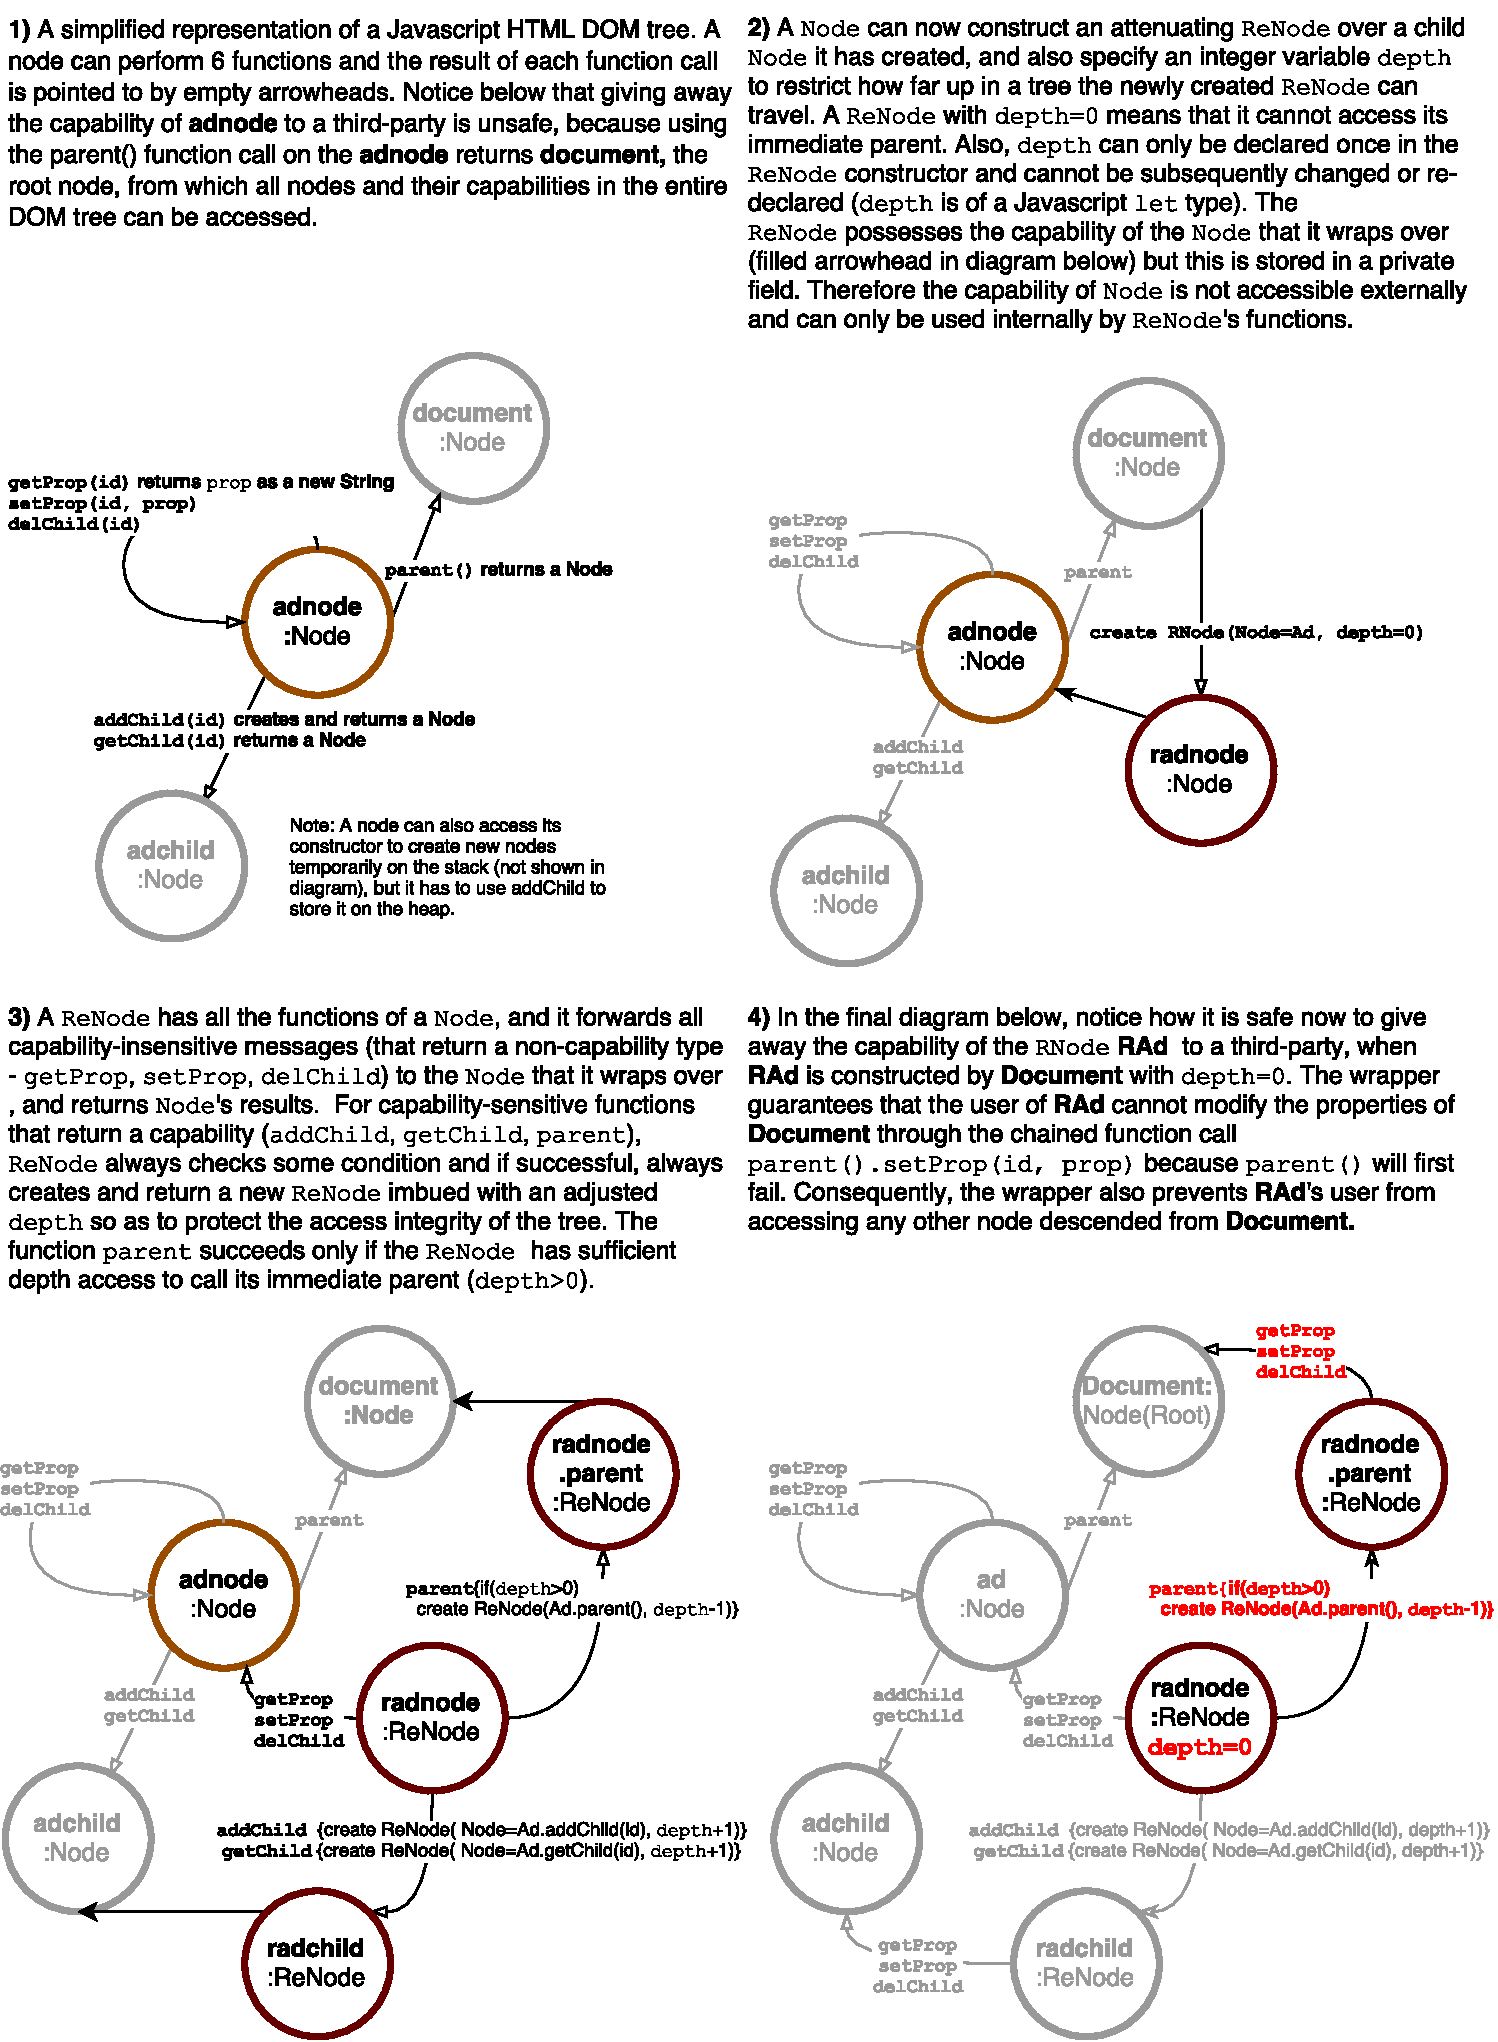
\includegraphics[width=\textwidth]{figures/DOM.pdf}
 \captionof{figure}{DOM Tree Example}\label{fig:figdom}
\end{minipage}
\clearpage

\subsubsection{DOM Tree Policies} \label{sec:dompolicies}
Here, we provide the policies for the DOM Tree, using our methodology and Hoare tuples. The use of ":" indicates the variables of the LHS of ":" belonging to a primitive type or class stated in the RHS of ":". Before we dive into the policies, we define the lookup of the k-th parent of a restricted node as follows:\\

\begin{logic}
\hr\\
\textbf{Definition ---[ReNode.parent]}\\
Given rn,rn$'$:ReNode, k:\lonat, then [ rn.parent\losup{k} = rn$'$ \loiff\ \=(k $\geq$ 1 \loand\ rn.parent.parent\losup{k-1} = rn$'$) \loor\\
\>(k = 0 \loand\ rn = rn$'$) ] \\
\hr
\end{logic}
\\
This definition says that given a superscript \losup{k} placed on a \sf{parent}, the result on the RHS of such a look up is the restricted node's parent on the LHS called \sf{k} times; if \sf{rn'} refers to the same restricted node as \sf{rn}, then k = 0.
\paragraph{Policies for calling and modifying nodes}
The following two policies describe the condition under which an Object or ReNode may call methods on a node.\\

\begin{logic}
\hr\\
\emp{Policy ---[Object calls Node]}\\
\loforall o:Object, \loforall n:Node. [ \=MayCall(o,n) \loand\ Dom(S,n) \loand\ \loforall s. [ s\loin S \loimplies s:ReNode ]\\
\>\loimplies\\
\>\loexists rn:ReNode. [ rn\loin S \loand\ MayCall(o,rn) \loand\ MayCall(rn,n) ] ]\\
\end{logic}
\\
\begin{logic}
\emp{Policy ---[ReNode calls Node (Necessary Condition)]}\\
\loforall rn:ReNode, \loforall n:Node. [ \=MayCall(rn,n) \loimplies\
\loexists rn$'$:ReNode. [ MayCall(rn,rn$'$) \loand\ rn$'$.node = n ] ]\\
\end{logic}
\\
\begin{logic}
\emp{Policy ---[ReNode calls Node (Sufficient Condition)]}\\
\loforall rn:ReNode, \loforall n:Node. [ \=rn.node = n \loimplies\
MayCall(rn,n) ]\\
\hr
\end{logic}

Policy [Object calls Node] says that if we have an object \sf{o} that can call the methods of node \sf{n}, and we have a set \sf{S} that dominates n such that all members in \sf{S} are of class \sf{ReNode}, then it implies that object \sf{o} must be able to call methods of a restricted node \sf{rn} out of \sf{S} and that \sf{rn} must able to call methods of \sf{n}. This just means that the chain of authority from \sf{o} to \sf{n} must involve \sf{rn} in the chain.\\
Policy [ReNode calls Node] says something about the last restricted node \sf{rn$'$} at the end of the chain of authority to n: that a restricted node \sf{rn} can call \sf{n} by calling another restricted node \sf{rn$'$} that points to \sf{n}. That is, a restricted node \sf{rn} that points to a node \sf{n} (\sf{rn.node = n)} \\

\paragraph{Policy for restricted node calling other restricted nodes}
\begin{logic}
\hr\\
\emp{Policy ---[ReNode calls ReNode (Necessary Condition)]}\\
\loforall rn,rn$'$:ReNode. [ \=MayCall(rn,rn$'$)\\
\>\loimplies\\
\>\loexists k,j:\lonat. [ \=(rn.parent\losup{k} = rn$'$.parent\losup{j}) \loand\ rn.depth \logeq k ] ]\\
\end{logic}\\

\begin{logic}
\emp{Policy ---[ReNode calls ReNode (Sufficient Condition)]}\\
\loforall k,j:\lonat, \loforall rn,rn$'$:ReNode. [ \=(rn.parent\losup{k} = rn$'$.parent\losup{j}) \loand\ rn.depth \logeq k \\
\>\loimplies\\
\>MayCall(rn,rn$'$) ]\\
\hr
\end{logic}\\

Policy [ReNode calls ReNode] describes a necessary condition and a sufficient condition for which a restricted node \sf{rn} may call another restricted node \sf{rn$'$}. This policy is subtle and says that a restricted node rn is allowed to navigate to all the descendants from all its accessible ancestors. $k$ is a natural number that indexes all the accessible ancestors of rn $k$ levels up the tree from rn, while we use another natural number $j$ that describes all the descendant nodes $j$ levels down the tree from a particular accessible ancestor. If rn$'$ is a direct descendant from rn, then k = 0. If \sf{rn$'$} is a direct ancestor of rn, then j = 0. An ancestor $k$ levels up the tree is only accessible if rn has sufficient depth access (rn \logeq k); there are no restrictions on accessing the descendants $j$ levels down the tree from a particular accessible ancestor.\\


\hr
\paragraph{Policy for reasoning about new paths from ReNodes}
\begin{logic}
\hr\\
\emp{Policy ---[Domination No Leaked Paths from ReNode]}\\
\loforall n:Node, RND$_{old}$. \=[ Dom(RND$_{old}$,n) \loand\ \loforall s. [ s\loin RND$_{old}$\loimplies s:ReNode ]\\
\>\{ \texttt{\textit{code}} \}\\
\loexists RND$_{new}$. [ \=Dom(RND$_{new}$,n) \loand\ \loforall s$'$\loin RND$_{new}$. [ \=s$'$:ReNode \loand\\
\>\loexists s$''$\loin RND$_{old}$, \loexists k,j:\lonat. [ \=(s$'$.parent\losup{k} = s$''$.parent\losup{j})  \loand\ (s$''$.depth \logeq j) \loand\\
\>\>(s$'$.depth = s$''$.depth - j + k) ] ] ] ]\\
\hr
\end{logic}

This policy is a very important security policy of the DOM Tree pattern.
The policy confines all possible paths to a node \sf{n} that might arise from running \textit{any} code, if all members in the initial set that dominates n belong to class \sf{ReNode}.
For all restricted nodes in the new dominating set, they must have been descended from some restricted node (\sf{s$''$.parent\losup{j}}), where (\sf{s$''$.parent\losup{j}}) is accessible from a restricted node s$''$ in the old dominating set (\sf{s$''$.depth \logeq j}). The policy says that an accessible ancestor \sf{s$''$} from a restricted node \sf{s$'$} in the old dominating set is indexed by a depth level j so that the accessible ancestor would inherit a depth level j higher than the depth level of \sf{s$''$}---(\sf{s$''$.parent\losup{j}.depth = s$''$.depth - j}). For a newly created restricted node \sf{s$'$} in the new dominating set that is descended k levels down from one of these accessible ancestors, it would thus inherit a depth of (\sf{s$''$.depth - j + k}). In other words every restricted node in the new dominating set must fall into one of these categories:
\begin{itemize}
\item a newly created restricted node descended k levels down directly from a restricted node in the old dominating set---\textbf{(j = 0, k > 0)}
\item a newly created restricted node descended k levels down from some restricted node that is an accessible ancestor j levels up of a restricted node from the old dominating set---\mbox{\textbf{(j > 0, k > 0)}}.
\item a new created restricted node that is a direct ancestor from a restricted node in the old dominating set---\textbf{(j > 0, k = 0)}
\item a restricted node in the new dominating set is also a member of the old dominating set---\textbf{(j = 0, k = 0)}
\end{itemize}
The argument for the policy is as follows: given a set of initial restricted nodes, we know by definition of the callable methods of a restricted node such that it can only create, store and return the capabilities of newly created restricted nodes, or return a \sf{null} value, or return a \sf{String} value, in \textbf{all} of its methods.\\

The policies for these methods can be found in \cref{renodemethods}. The execution policies in 
\cref{renodemethods} imply that all newly created restricted nodes from existing restricted nodes must obey certain policies (such as inheriting an incremented depth from its creator restricted node if its a child, or inheriting a decremented depth if it is a parent). Therefore, all restricted nodes in the new dominating set, if created during the unknown code execution, must be connected to a creator restricted node in the old dominating set through some path formed from the policies in \cref{renodemethods}, or is already a member of the old dominating set, no matter what kind of code execution. 
\paragraph{Policies for methods of ReNode}\label{renodemethods}
The six methods in ReNode are described in the policies as follows:\\

\begin{logic}\hr\\
\emp{Policy ---[Execution of ReNode.parent]}\\
\loforall rn:ReNode, \loexists i:String. \loforall s. [ \=(rn.depth > 0)\\
\>\{\texttt{s = rn.parent()}\} \\
\>(s:ReNode) \loand\ (s = rn.parent) \loand\ (s.child(i) = rn) \loand\\
\>(s.node = rn.node.parent) \loand\\
\>(s.depth = rn.depth - 1)\\
\>\loor\\
\>s = \texttt{null} ]\\
\end{logic}\\
This policy says that the pre-condition creating a parent restricted node requires that the creator restricted node must have a depth level of more than 0. The post-conditions are that the newly created parent restricted node would be pointing towards a node that is the parent node of the node that its creator is pointing towards, and the newly created parent restricted node inherit the depth level of its creator restricted node decremented by 1.\\

\begin{logic}
\emp{Policy ---[Execution of ReNode.setProp]}\\
\loforall rn:ReNode, \loforall i,j:String. [ \textit{true} \{\texttt{rn.setProp(i,j)}\} rn.node.prop(i) = j ]\\
\end{logic}

\begin{logic}
\emp{Policy ---[Execution of ReNode.getProp]}\\
\loforall rn:ReNode, \loforall i,j:String. [ \textit{true} \{\texttt{j = rn.getProp(i)}\} j = rn.node.prop(i) ]\\
\end{logic}

\begin{logic}
\emp{Policy ---[Execution of ReNode.addChild]}\\
\loforall rn,rn$'$:ReNode, \loforall i:String. [ \=\textit{true}\\
\>\{\texttt{rn$'$ = rn.addChild(i)}\}\\
\>(rn$'$ = rn.child(i)) \loand\ (rn$'$.parent = rn) \loand\\
\>(rn$'$.node = rn.node.child(i)) \loand\\
\>(rn$'$.depth = rn.depth + 1) ]\\
\end{logic}

\begin{logic}
\emp{Policy ---[Execution of ReNode.getChild]}\\
\loforall rn:ReNode, \loforall i:String, \loforall s. [ \=\textit{true}\\
\>\{\texttt{s = rn.getChild(i)}\}\\
\>(s:ReNode) \loand\ (s = rn.child(i)) \loand\ (s.parent = rn) \loand\\
\>(s.node = rn.node.child(i)) \loand\\
\>(s.depth = rn.depth + 1) ]\\
\>\loor\\
\> s = \texttt{null} ]\\
\end{logic}

\begin{logic}
\emp{Policy ---[Execution of ReNode.delChild]}\\
\loforall rn:ReNode, \loforall i:String. [ \textit{true} \{\texttt{rn.delChild(i)}\} \=rn.child(i) = \texttt{null} \loand\\
\> rn.node.child(i) = \texttt{null} ]\\
\end{logic}

\hr
\paragraph{Policy for ReNode Constructor}\label{renodeconstructor}
The constructor for \sf{ReNode} is private to the module and class \sf{ReNode}. This means that an unknown object cannot directly use the constructor of \sf{ReNode} even if it holds the capability of an object belonging to class ReNode, unless the unknown object is in the same module as ReNode.\\

\begin{logic}
\hr\\
\emp{Policy ---[Constructor of new ReNode]}\\
\loforall rn:ReNode, \loforall n:Node, \loforall k:\lonat. [ \textit{true} \{\texttt{rn = ReNode(n,k)}\} \=rn.node = n \loand\\
\>rn.depth = k \loand\\
\>rn.parent = \texttt{null} ]\\
\end{logic}

\hr
\paragraph{Policies on immutable properties}\label{policy_immutable}
The following policies describe the properties that hold in any state of execution. Namely, a node that a restricted node points to will never change [Immutability of ReNode.node], its ancestor(s) will never change [Immutability of ReNode.parent\losup{k}], its depth will never change [Immutability of ReNode depth], and the depth of a restricted node will never be less than 0 [Invariant of minimum ReNode depth].\\

\begin{logic}
\emp{Policy ---[Immutability of ReNode.node]}\\
\loforall rn:ReNode, \loforall n:Node. [ rn.node = n \{\texttt{code}\} rn.node = n ]\\
\end{logic}

\begin{logic}
\emp{Policy ---[Immutability of ReNode.parent\losup{k}]}\\
\loforall rn,rn$'$:ReNode, \loforall k:\lonat. [ rn.parent\losup{k} = rn$'$ \{\texttt{code}\} rn.parent\losup{k} = rn$'$ ]\\
\end{logic}

\begin{logic}
\emp{Policy ---[Immutability of ReNode depth]}\\
\loforall rn:ReNode, \loforall k:\lonat. [ rn.depth = k \{\texttt{code}\} rn.depth = k ]\\
\end{logic}

\begin{logic}
\emp{Policy ---[Immutability of minimum ReNode depth]}\\
\loforall rn:ReNode. [ \textit{true} \{\texttt{code}\} rn.depth \logeq 0 ]\\
\end{logic}

\hr\\

\subsection{Reasoning about the DOM Tree with unknown code using our policies}\label{sec:treereasoning}
In this subsection, we will now discuss how the policies we have developed in \cref{sec:dompolicies} allow us to reason about  the use of restricted nodes of class \sf{ReNode} to attenuate authority of nodes of class \sf{Node} is a DOM tree. In particular, we can argue that authority is attenuated in the presence of the execution of unknown code. We also believe that the argument we have put forth using our logics is relatively simple, and natural to a programmer, compared with the corresponding works by Devriese et al.\cite{devriese2016} that uses Kripke world logics and Swasey et al.\cite{swasey2017} that builds on the Iris framework for concurrent separation logic. Furthermore, our framework allows us to reason about unknown code without needing to deploy more sophisticated tools of more advanced logic frameworks. In the code below, we create another DOM Tree example with the following structure:\\
\begin{minipage}{\textwidth}
\centering
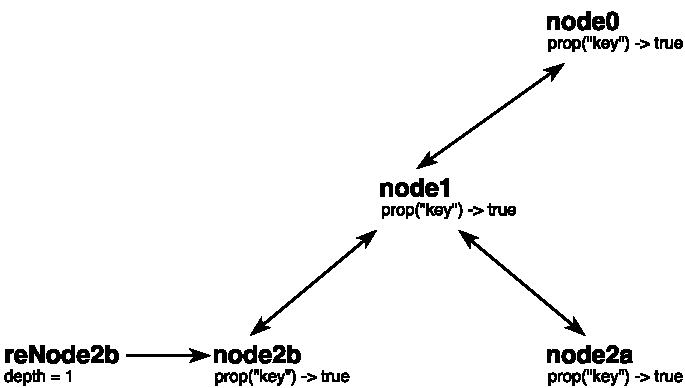
\includegraphics[width=0.80\textwidth]{figures/assertion.pdf}
 \captionof{figure}{DOM Tree Example With Unknown Code}
  \label{DOM example}
\end{minipage}
\begin{lstlisting}[numbers = left]
node0 = Node.createRoot("node0")
node0.setProp("key", "true")

node1 = node0.addChild("node1")
node1.setProp("key", "true")

node2a = node1.addChild("node2a")
node2a.setProp("key", "true")

node2b = node1.addChild("node2b")
node2b.setProp("key", "true")

reNode2b = ReNode(node2b, 1) //reNode2b given depth level of 1

// we have a mystery object o, which we do not trust
// o has a mystery method that takes an object reference as an argument
// we give o the capability of node2b, and o attempts to execute a mystery method on renode2b:

o.mystery0(renode2b)

&\textbf{Assertion 1:}& node0.getProp("key") = "true"
&&
\end{lstlisting} \captionof{figure}{Code for DOM Tree Pattern with unknown provenance}
\vspace{0.5em}
It is unsafe to hand the capability of \sf{node2b} directly to an untrusted agent, because it is possible the properties and state of the entire DOM tree would be compromised, in particular the root node \sf{node0} whose properties and state we want to protect in this example. Note that an untrusted agent having the direct capability of \sf{node2b} implies that the untrusted agent is able to obtain the direct capability of \sf{node1}, \sf{node2a}, and \sf{node0}, because \sf{node2b} has methods that freely gives those capabilities to any caller.\\

 How then, can we allow an untrusted agent whose object and code we do not know, to safely modify the properties of \sf{node2b},  and some other nodes (\sf{node2a} and \sf{node1}), whose properties are not critical and we do not mind being modified, but \textbf{not} allow the untrusted agent to modify the properties of \sf{node0} which are critical and which we want to protect?\\

We will accomplish this by creating an attenuating restricted node object called \sf{reNode2b}, which points to \sf{node2b} and has a depth level of \sf{1} (\sf{reNode2b.node = node2b, reNode2b.depth = 1}). On \texttt{line 19}, we pass \sf{reNode2b} to an object \sf{o} of unknown provenance. While we do not know exactly how \sf{o} might make use of \sf{reNode2b}, we can comfortably argue that the properties of \sf{node0} have been preserved after the execution of an unknown \sf{mystery} function by \sf{o}. However, because we have configured \sf{reNode2b} to allow the unknown object to potentially modify the properties of \sf{node2a}, \sf{node2b} and \sf{node1}, we do not know if the properties of \sf{node2a}, \sf{node2b} and \sf{node1} have been preserved.\\

We argue that \textbf{Assertion 1} at \texttt{line 21} holds, i.e. after execution of a piece of unknown code, we know that \sf{node0.getProp("key") = "true"}. We now sketch the proof of this assertion below.\\

We begin by stating several facts at \texttt{line 18}, before the execution of \sf{mystery}. namely:
\begin{itemize}
\item \textbf{F1}: \sf{node2b.getProp("key") = true}
\item \textbf{F2}: \sf{reNode2b.depth = 1}
\item \textbf{F3}: \sf{reNode2b.node = node2b}
\item \textbf{F4}: \sf{reNode2b.parent.node = node1}
\item \textbf{F5}: \sf{reNode2b.parent.child("node2a").node = node2a}
\item \textbf{F6}: \sf{reNode2b.parent.parent.node = node0}
\end{itemize}

Then at \texttt{line 21}, we consider the effects of the \sf{mystery} function. We argue that:
\begin{itemize}
\item \textbf{(A)}: \textbf{F1} is preserved, unless \textbf{\sf{MayCall(o,node0)}} holds at line 19. This is based on the observation below:\\
\begin{logic}
\hr\\
\emp{Observation ---[Node Property Modification]}\\
\loforall n:Node, \loforall o:Object. [ [ n.prop(i) = j \{ \texttt{o.\textit{code}} \} n.prop(i) \loneq\ j ] \loimplies\ MayCall(o,n) ]\\
\hr
\end{logic}

which follows from our Lemma [Field Modification Requires Authority], which says that if a property of a node \sf{n} is modified after the execution of some code by object \sf{o}, then it implies \sf{o} must be able to invoke a method on \sf{n}.
\end{itemize}
Therefore, to show that \textbf{Assertion 1} at \texttt{line 21} holds, it is sufficient to show that at \texttt{line 19}, the assertion MayCall(o,node0) does not hold. We will show this by contradiction.\\

Let us assume during execution of the \sf{mystery} function in \texttt{line 19}; at some point:
\begin{itemize}\item \textbf{(B)}: \sf{MayCall(o,node0)}\end{itemize}

During execution of the method call \sf{mystery}, the receiver is \sf{o}, and the method argument is \sf{reNode2}. Moreover, \sf{node0} was created before \sf{o}. Therefore, within this frame, it holds that : 
\begin{itemize}
\item \textbf{(C)}: \sf{Dom(\{reNode2b\}, node0)}
\item \textbf{(D)}: \sf{reNode2b:ReNode}
\end{itemize}

Applying \textbf{Policy [Object calls Node]} on \textbf{(C)} and \textbf{(D)}, we obtain:
\begin{itemize}
\item \textbf{(E)}:
\begin{logic}
MayCall(o,node0) \loimplies\ MayCall(o,reNode2b) \loand\ MayCall(reNode2b,node0)
\end{logic}
\end{itemize}
From \textbf{(D)} and \textbf{(E)} and applying \textbf{Policy [ReNode calls Node]}, we obtain that there exists a rn:ReNode such that:
\begin{itemize}\item \textbf{(F)}: \sf{MayCall(renode2b,node0)} \loimplies \sf{MayCall(renode2b,rn) \loand\ rn$'$.node = node0}\end{itemize}
From \textbf{(D)} and by applying \textbf{Policy [ReNode calls ReNode]} on \textbf{(F)}, we know that there exists a k,j:\lonat\ such that:
\begin{itemize}\item \textbf{(G)}:
\begin{logic}
MayCall(renode2b,rn) \loimplies\ reNode2b.parent\losup{k} = rn.parent\losup{j} \loand\ reNode2b.depth \logeq k
\end{logic}
\end{itemize}
From \textbf{(G)}, and \textbf{(F2)} \sf{which says reNode2b.depth = 1}, we obtain that:
\begin{itemize}\item \textbf{(H)} k = 0 \loor\ k = 1
\item Using proof by cases,\\
\begin{logic}
\textbf{1\losup{st} case} k = 0, \=then for all rn$'$ such that rn$'$.parent\losup{j} = reNode2b,\\
\>we have that rn$'$ are descendants of reNode2b,\\
\>and therefore from \textbf{(F3) and (F6)}, we also know:\\
\>\textbf{rn$'$.node \loneq\ node0}
\\
\textbf{2\losup{st} case} k = 1, \=then for all rn$'$ such that rn$'$.parent\losup{j} = reNode2b.parent,\\
\>we have that rn$'$ are descendants of reNode2b.parent,\\
\>and therefore from \textbf{(F4) and (F6)}, we also know:\\
\>\textbf{rn$'$.node \loneq\ node0}
\end{logic}
\item Therefore, \textbf\sf{{rn$'$.node \loneq\ node0}} from proof by cases.
\end{itemize}
We thus obtain a contradiction from \textbf{(F)}, and we know that assumption \textbf{(B)} must be false:
\begin{itemize} \item \textbf{\sf{\loneg MayCall(o,node0)}} \end{itemize}
Consequently, from \textbf{(A)}, we know the properties of \sf{node0} is preserved.\\

Note that in the above steps we used without mentioning explicitly that the parent and depth fields of all restricted nodes belonging to \sf{ReNode} are immutable. Our \textbf{Policies on immutable properties} in \cref{policy_immutable} tell us that the properties \textbf{(F2-F6)} are preserved throughout execution of the body of the \sf{mystery} function, and the minimum depth of all restricted nodes must be greater than 0.
\clearpage
\subsection{Caretaker and Membrane Patterns}

The Caretaker pattern originally appeared in Redell's 1974 work {\cite{redell1974}, but features prominently along with its more advanced Membrane pattern in the works of \cite{miller2006,murray2010,swasey2017}. Unlike the previous DOM Tree pattern, protected objects in the Caretaker and Membrane pattern are now no longer necessarily ordered in some hierarchical access structure. Consequently, the attenuating 'caretaker' and 'membrane' objects do not try to maintain the integrity of some hierarchy structure, as compared to the attenuating ReNode object in the DOM Tree, where it maintains hierarchy of the Tree by adjusting the depth of ReNodes that it can return (parent ReNodes have decremented depths while child ReNodes have incremented depths).\\

The Caretaker merely fulfils the simple task of 1) masking the protected object's direct capability, and 2) only forwarding messages to the protected object according to some condition in an associated lock object. Note that a simple caretaker object forwards messages without analysing the contents of the messages, i.e. messages can contain capabilities. The Membrane pattern on the other hand, shares some similarities from both the DOM Tree pattern and Caretaker pattern. The Membrane pattern is identical to the Caretaker pattern in the sense that it is meant to mask the protected object's direct capability and forward messages to the protected object, but with the exception that it does not forward messages that contain capabilities without first 'wrapping' those capabilities within new membranes. The membrane attenuating object can create more membranes (or deep attenuating objects) that is similar to the DOM Tree pattern where a restricted node creates more restricted nodes when accessing different parts of the tree.\\

We first show the important policies for the Caretaker pattern in \cref{sec:caretakerpolicies} and a visual illustration of it in \cref{fig:figcaretaker}. The policies for the Membrane pattern can be found next in \cref{sec:membranepolicies}, and its visual illustration in \cref{fig:figmem}. In the Caretaker pattern, while the status of the lock object \sf{Carol-CT-Lock} for the caretaker object \sf{Carol-CT} is disabled (\sf{Carol-CT.status = false}), object \sf{Bob} can pass his own capability to \sf{Carol} using \sf{Carol-CT}, and consequently, with \sf{Bob}'s capability, \sf{Carol} can pass the capability of \sf{Diane}, which \sf{Carol} initially holds, to \sf{Bob}. \textit{After} the \sf{Lock} object is enabled (\sf{Carol-CT.status = true}), \sf{Carol-CT} no longer forwards messages to \sf{Carol}. However, because \sf{Bob} has transferred his own capability to \sf{Carol}, and \sf{Carol} has transferred the capability of \sf{Diane} to \sf{Bob} during \sf{Carol-CT.status = false}, even after \sf{Carol-CT.status = true}, Carol can continue to communicate with \sf{Bob}, and \sf{Bob} can continue to communicate with \sf{Diane}, because these objects can store the capabilities they have received for future use. For the Membrane example however, for all messages that contain capabilities, those messages will be attenuated before being forwarded. When \sf{Bob} tries to send his own capability to \sf{Carol} through the membrane \sf{Carol-M}, \sf{Carol-M} will wrap the capability of \sf{Bob} within the message in a new membrane \sf{Bob-M} and lock \sf{Bob-M-Lock}, and forward the new membrane  \sf{Bob-M} to \sf{Carol}, and when \sf{Carol} tries to send the capability of \sf{Diane} to \sf{Bob} using \sf{Bob-M}, a similar membrane \sf{Diane-M} and lock object is created by \sf{Bob-M}. When \sf{Alice} decides to disable \sf{Carol-M} by setting \sf{Carol-M-Lock = true}, the disabling action can propagate to all membranes descended from \sf{Carol-M}, thereby preventing communication from \sf{Carol} to \sf{Bob} and \sf{Bob} to \sf{Diane}.

\clearpage
\begin{minipage}{\textwidth}
\subsubsection{Caretaker Pattern - Illustration}\label{sec:figcaretaker}
\small Here, we illustrate in more detail an example of the Caretaker pattern. The code can be found in \cref{sec:code_Caretaker}.\\
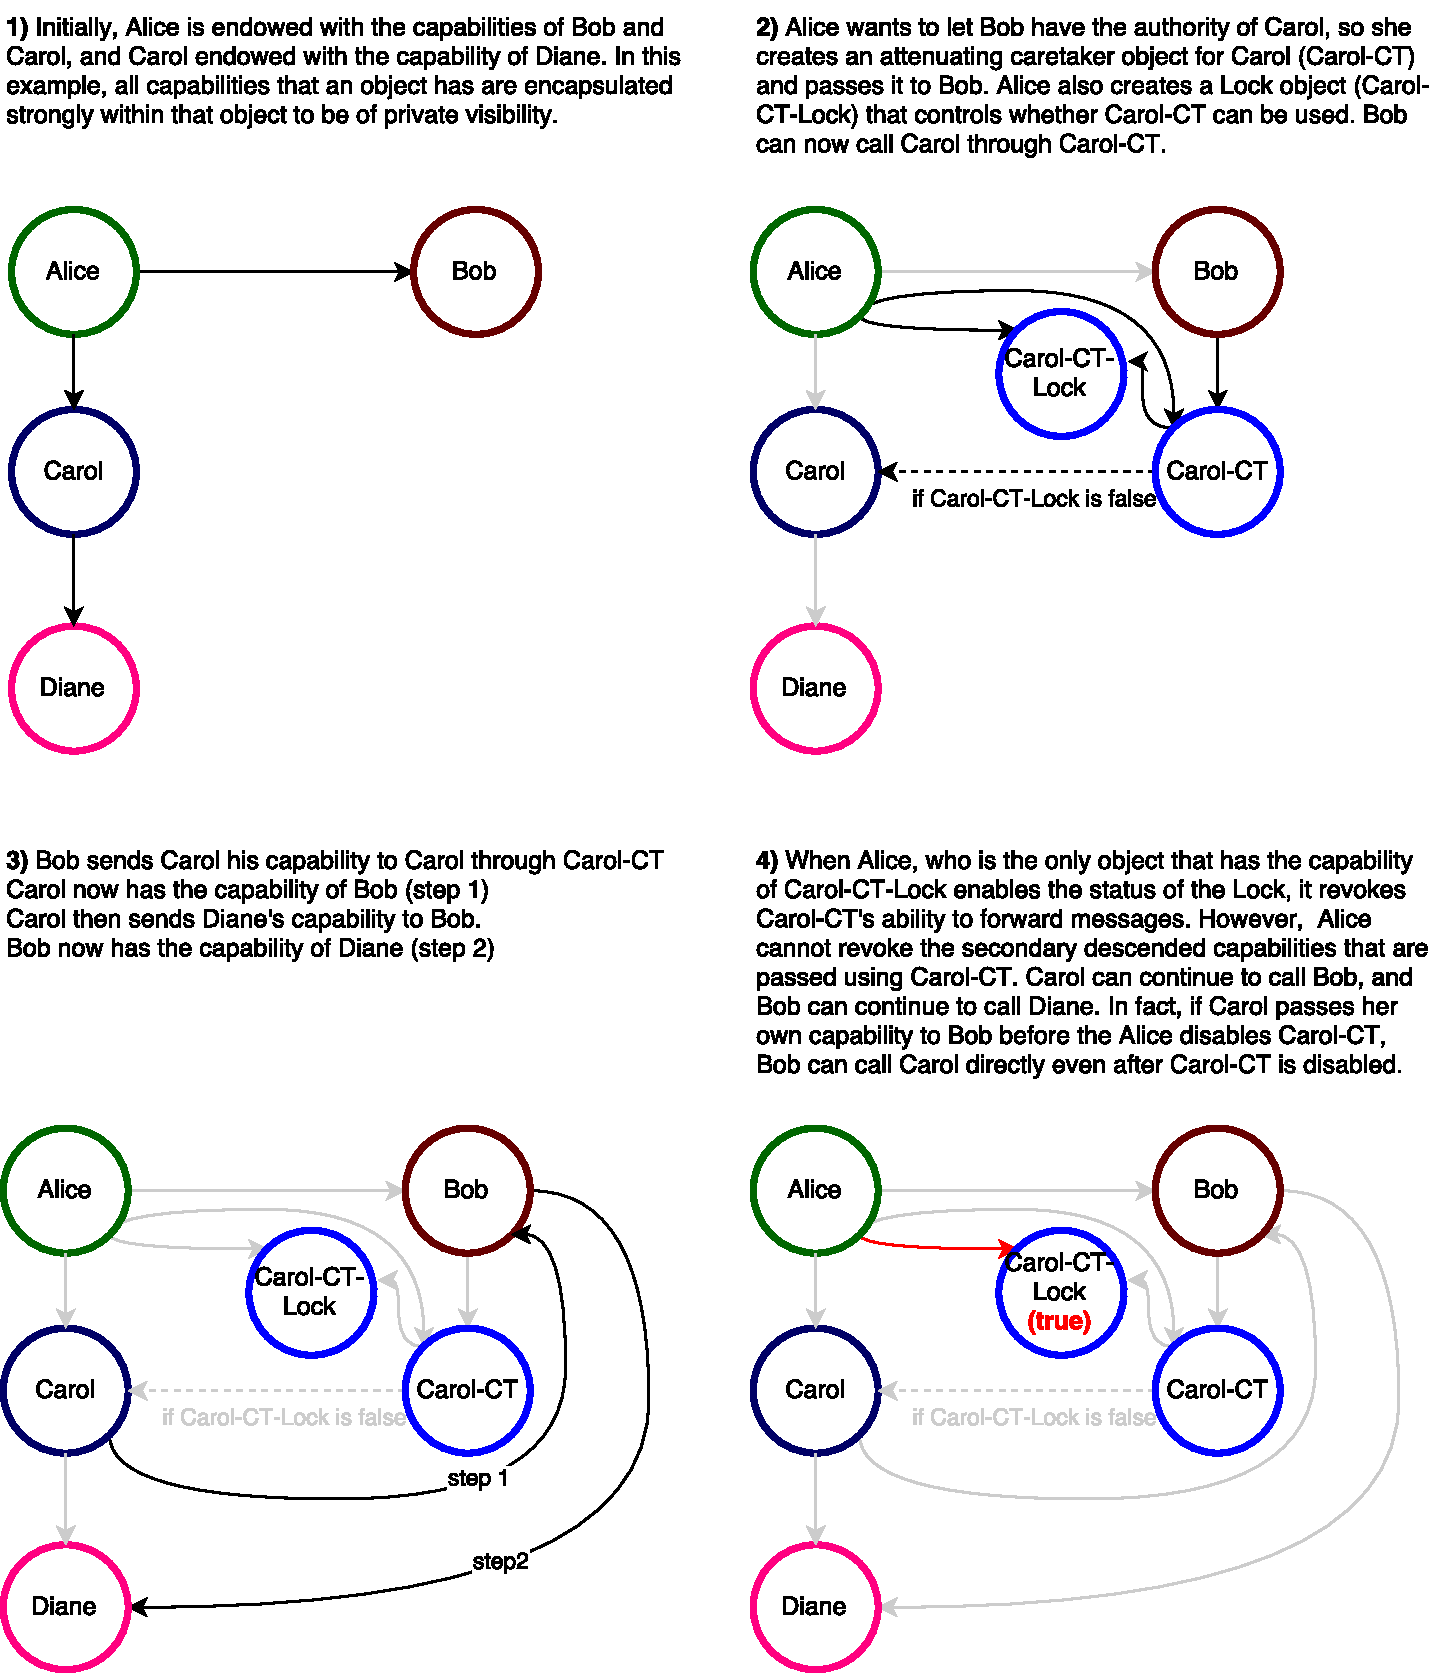
\includegraphics[width=1.05\textwidth]{figures/Caretaker.pdf}
 \captionof{figure}{Caretaker Pattern}
  \label{fig:figcaretaker}
\end{minipage}
\clearpage
\subsubsection{Caretaker Pattern - Policies}\label{sec:caretakerpolicies}
Here we show the important policies for the Caretaker pattern, where we also say how the Caretaker might leak paths in \textbf{Policy [Possible Leaked Paths from Caretaker]}. Path leakage is possible because the caretaker might possibly return the capability of its protected object o$'$ from some method call forwarded to o$'$, when o$'$ has a method that exposes its own capability; i.e. the caretaker does not create deep attenuating objects to mask capabilities returned by its protected object, or messages containing capabilities passed by its caller.\\

\begin{logic}
\emp{Policy ---[Object calls Node]}\\
\loforall o,o$'$:Object, \loforall n:Node. [ \=MayCall(o,o$'$) \loand\ Dom(S,o$'$) \loand\ \loforall s. [ s\loin S \loimplies s:Caretaker ]\\
\>\loimplies\\
\>\loexists ct:Caretaker. [ ct\loin S \loand\ MayCall(o,ct) \loand\ MayCall(ct,o$'$) ] ]\\
\end{logic}

\begin{logic}
\emp{Policy ---[Possible Leaked Paths from Caretaker]}\\
\loneg\ [ \loforall o:Object, S$_{old}$. \=[ Dom(S$_{old}$,o) \loand\ \loforall s. [ s\loin S$_{old}$\loimplies s:Caretaker ]\\
\>\{ \texttt{\textit{code}} \}\\
\>\loexists S$_{new}$. [ \=Dom(S$_{new}$,n) \loand\ \loforall s$'$\loin S$_{new}$. [ \=s$'$:Caretaker ] ] ] ]\\

\end{logic}

\begin{logic}
\emp{Policy ---[Caretaker calls Caretaker.target (Necessary Condition)]}\\
\loforall c:Caretaker. [ MayCall(c,c.target) \loimplies\ c.lock.status = \texttt{false} ]\\
\end{logic}

\begin{logic}
\emp{Policy ---[Execution of Lock.lock()]}\\
\loforall k:Lock. [ \=\textit{true} \{\texttt{k.lock()}\} k.status = \texttt{true} ]\\
\end{logic}

\begin{logic}
\emp{Policy ---[Constructor of new Caretaker]}\\
\loforall ct:Caretaker, \loforall o:Object, \loforall k:Lock. [ \textit{true} \{\texttt{ct = Caretaker(o,k)}\} \=ct.target = o \loand\ ct.lock = k ]\\
\end{logic}

\begin{logic}
\emp{Policy ---[Immutability of Caretaker.lock]}\\
\loforall c:Caretaker. [ \=c.lock = k \{\texttt{\textit{code}}\} c.lock = k ]\\
\end{logic}

\begin{logic}
\emp{Policy ---[Immutability of Caretaker.target]}\\
\loforall c:Caretaker. [ \=c.target = o \{\texttt{\texttt{\textit{code}}}\} c.target = o ]\\
\hr
\end{logic}
\begin{minipage}{\textwidth}
\subsubsection{Membrane Pattern - Illustration}\label{sec:figmem}
\small Here, we illustrate in more detail an example of the Membrane pattern. The code can be found in \cref{sec:code_Membrane}.\\
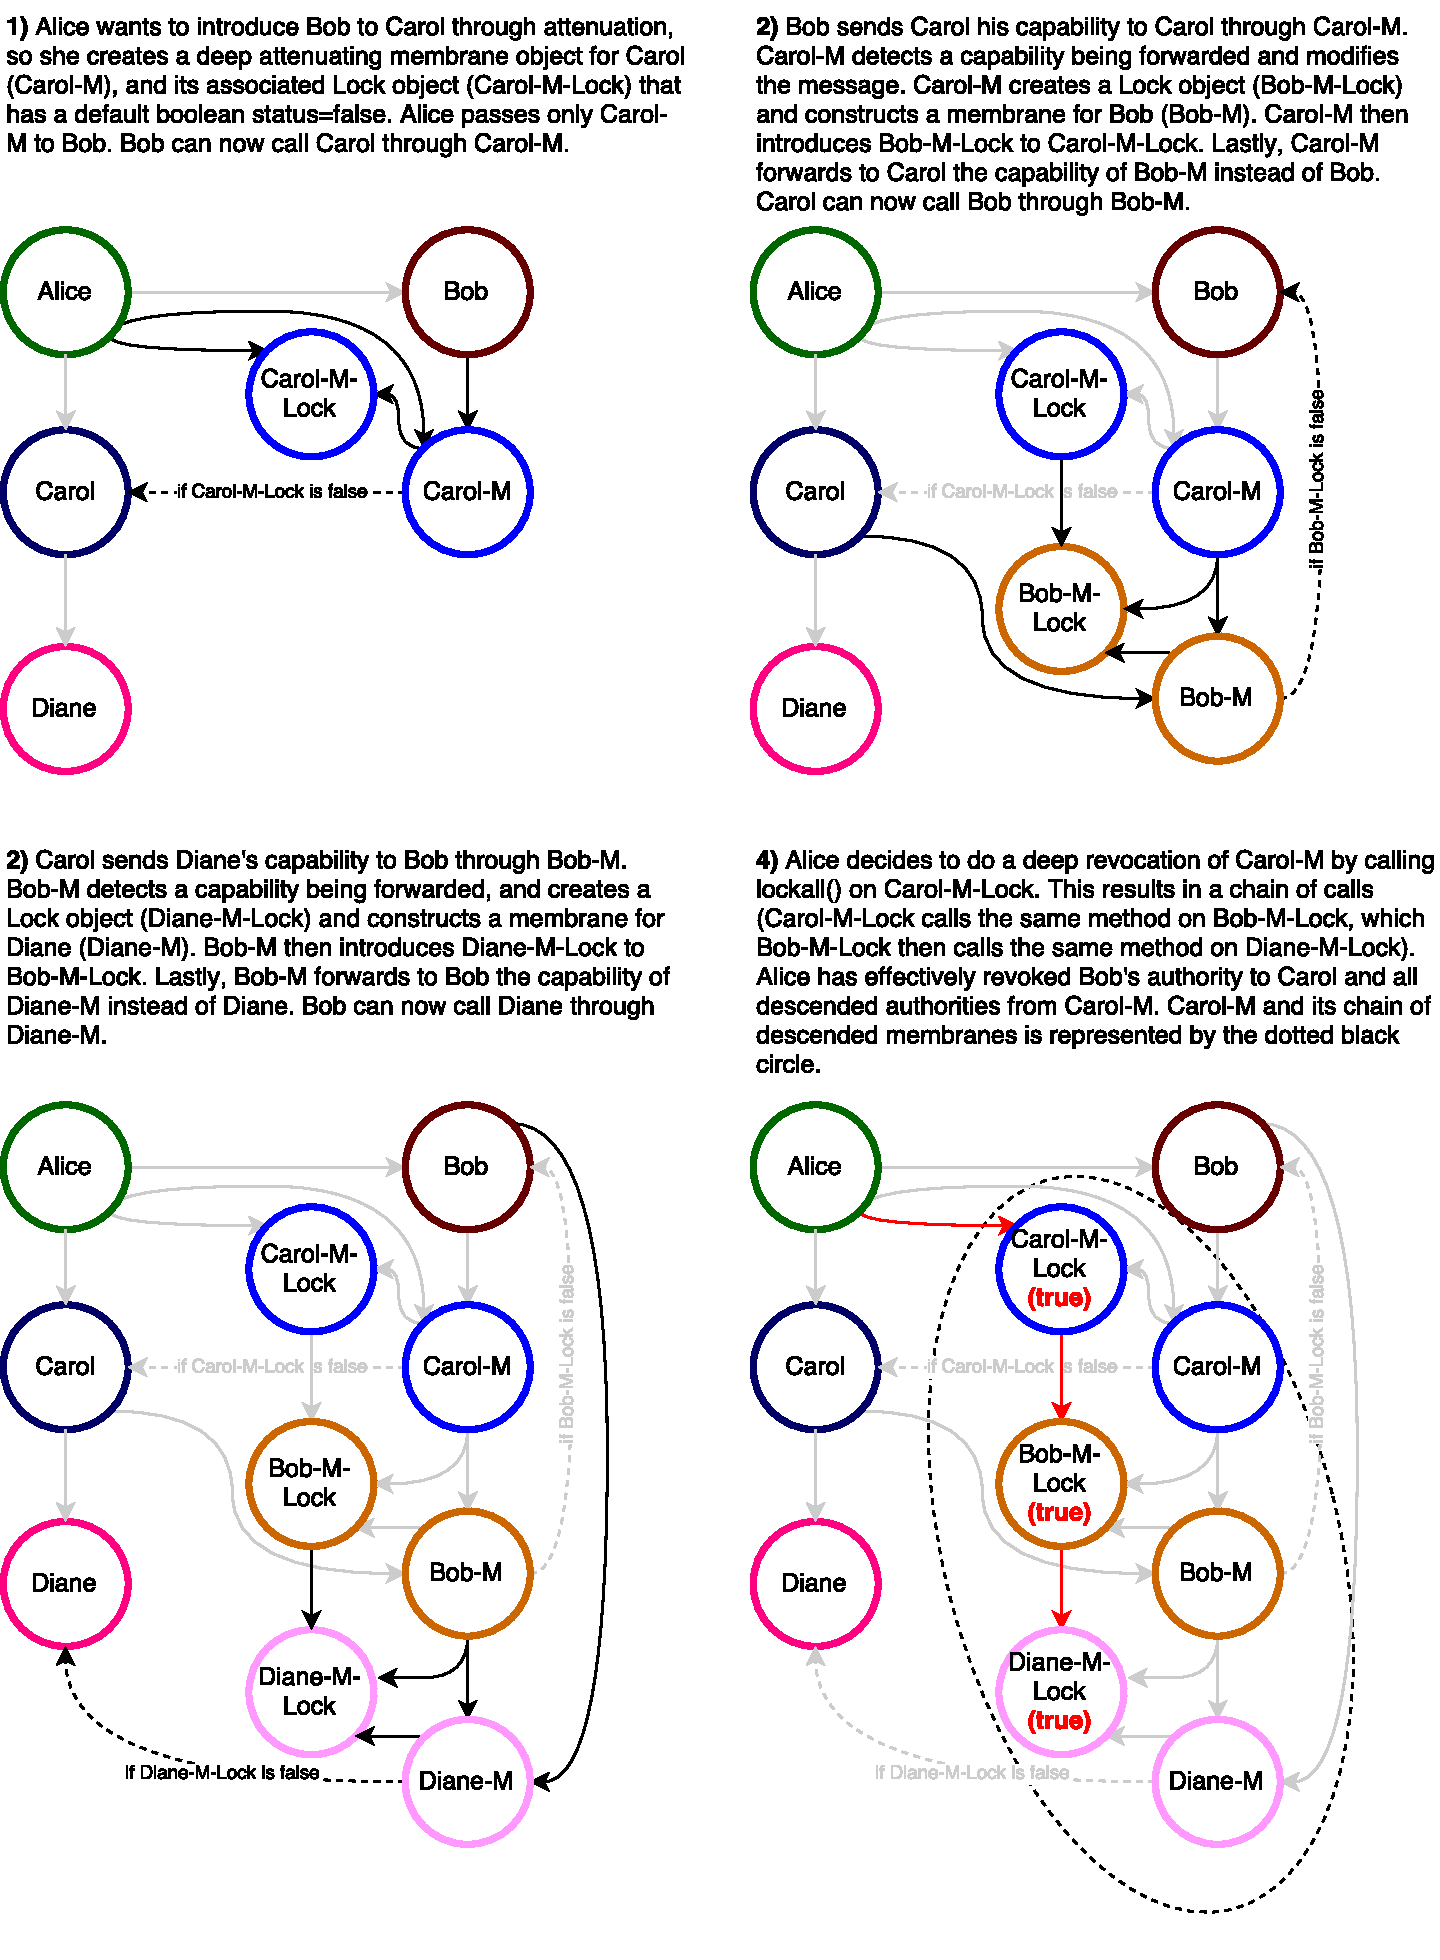
\includegraphics[width=1.05\textwidth]{figures/Membrane.pdf}
 \captionof{figure}{Membrane Pattern}
   \label{fig:figmem}
\end{minipage}
\clearpage
\subsubsection{Membrane Pattern - Policies}\label{sec:membranepolicies}
Here we show the important policies for the Membrane pattern. Unlike the Caretaker pattern, a Membrane does not leak capabilities because the membrane creates deep attenuating new membranes to mask capabilities returned by its protected object, and do so also for capabilities in messages passed by its caller. A membrane that creates new membranes also creates the associated lock objects for the new membranes, and passes the capabilities of these new locks to its own associated lock object \sf{k}. Therefore when some other object calls the method \sf{lockall()}\\on the lock object \sf{k}, \sf{k} will recursively call the same method on all lock objects that it has.
 
Therefore, every membrane and lock object has a ghost field \sf{parent}: \begin{itemize}
\item The ghost field \sf{parent} of a membrane object \sf{m$'$} points to a membrane \sf{m} if the constructor for \sf{m$'$} is called  by \sf{m}, otherwise it points to \sf{null}
\item The ghost field \sf{parent} of a lock object \sf{k$'$} points to a lock \sf{k} if the constructor for \sf{k$'$} is called by a membrane \sf{m}, where \sf{m.lock = k}, otherwise it points to \sf{null}
\end{itemize}

\begin{logic}
\emp{Policy ---[Object calls Object$'$]}\\
\loforall o,o$'$:Object. [ \=MayCall(o,o$'$) \loand\ Dom(S,o$'$) \loand\ \loforall s. [ s\loin S \loimplies s:Membrane ]\\
\>\loimplies\\
\>\loexists m:Membrane. [ m\loin S \loand\ MayCall(o,m) \loand\ MayCall(m,o$'$) ] ]\\
\end{logic}

\begin{logic}
\emp{Policy ---[Domination No Leaked Paths from Membrane]}\\
\loforall o:Object, MEM$_{old}$. \=[ Dom(MEM$_{old}$,o) \loand\ \loforall s. [ s\loin MEM$_{old}$\loimplies s:Membrane ]\\
\>\{ \texttt{\textit{code}} \}\\
\>\loexists MEM$_{new}$. [ \=Dom(MEM$_{new}$,n) \loand\ \loforall s$'$\loin MEM$_{new}$. [ \=s$'$:Membrane \loand\\
\>\>\loexists s$''$\loin MEM$_{old}$, \loexists k:\lonat. [ \=(s$'$.parent\losup{k} = s$''$) ] ] ] ]\\
\end{logic}

\begin{logic}
\emp{Policy ---[Membrane calls Membrane.target (Necessary Condition)]}\\
\loforall m:Membrane. [ MayCall(m,m.target) \loimplies\ m.lock.status = \texttt{false} ]\\
\end{logic}


\begin{logic}
\emp{Policy ---[Constructor of new Membrane]}\\
\loforall m:Membrane, \loforall o:Object, \loforall k:Lock. [ \textit{true} \{\texttt{m = Membrane(o,k)}\} \=m.target = o \loand\ m.lock = k ]\\
\end{logic}

\begin{logic}
\emp{Policy ---[Each Membrane in the Tree has an associated Lock in the same Tree]}\\
\loforall m,m$'$:Membrane, \loforall j:\lonat. [ m.parent\losup{j} = m$'$ \loiff\ m.lock.parent\losup{j} = m$'$.lock]\\
\end{logic}

\begin{logic}
\emp{Policy ---[Execution of Lock.lock()]}\\
\loforall k:Lock. [ \=\textit{true} \{\texttt{k.lock()}\} k.status = \texttt{true} ]\\
\end{logic}

\begin{logic}
\emp{Policy ---[Execution of Lock.lockall()]}\\
\loforall k:Lock. [ \=\textit{true} \{\texttt{k.lockall()}\} \loforall k$'$:Lock, \loforall j$>$0. [ k$'$.parent\losup{j} = k \loimplies\ k$'$.status = \texttt{true} ]\\
\end{logic}


\begin{logic}
\emp{Policy ---[Immutability of Membrane.lock]}\\
\loforall m:Membrane. [ \=m.lock = k \{\texttt{\textit{code}}\} m.lock = k ]\\
\end{logic}

\begin{logic}
\emp{Policy ---[Immutability of Membrane.target]}\\
\loforall m:Membrane. [ \=m.target = o \{\texttt{\texttt{\textit{code}}}\} m.target = o ]\\
\hr
\end{logic}

\section{Case Study of Ethereum / Solidity as a Non-OCap Model}\label{sec:ethereum}

\subsection{Motivation}
Recent widespread adoption of distributed ledger technology (blockchain) has created multiple decentralised, distributed computational platforms where millions of dollars are transacted over codified constructs called smart contracts. For example, as of 7 September 2017, Ethereum\cite{wood2014} is approximately a US\$30 billion blockchain platform with an in-built Turing-complete programming language that can be used to create and deploy such contracts.

\subsection{Solidity - Language for smart contracts}
Solidity\footnote{https://solidity.readthedocs.io/en/develop/} is a high-level language with a syntax similar to that of JavaScript and is designed to write smart contracts on the Ethereum Virtual Machine (EVM), the Turing-complete 256bit runtime environment of the Ethereum blockchain\footnote{Details on the Ethereum blockchain platform in our paper are based on the Etheruem white-paper: https://github.com/ethereum/wiki/wiki/White-Paper\\}.

\subsection{Objects in Solidity}
On the Ethereum blockchain, there are generally two types of accounts: "externally-owned accounts"(external accounts)  and "contract accounts"(contracts). We define these entities as objects because they encapsulate both state and behaviour. In terms of state, both types of accounts have an Ether balance (the currency of Ethereum) associated with them, while contract accounts differ from external accounts by having additional persistent contract storage that can store data such as integers and strings. In terms of behaviour, both types of accounts come with a predefined set of methods to transfer Ether, but contract accounts can have additional specified methods. The methods of external accounts can only be called by a person who has authenticated himself as the owner of the external account using a private key, while methods of contract accounts that are deployed on the blockchain can be called based on any conditions defined in the contract.
Hence, external accounts are controlled by public-private key cryptography, while contract accounts are controlled by their contract code. An external account has no code but can send messages to other external accounts or contract accounts by creating or signing a transaction. For contract accounts, everytime the contract account receives a message, its code activates, allowing it to read and write to its internal storage and sending other messages to other external accounts or contracts. Transactions can be triggered from both types of accounts, though contracts can only trigger transactions in response to other transactions that they have received. Therefore, all transactions in Ethereum can only originate from external accounts.

\subsubsection{Object References/Addresses} In Ethereum, the designations of all external account and contract objects are made of up a 20 bytes value. Hence, if we treat smart contracts and Ethereum accounts as objects, then these object references are not unforgeable---because anybody can specify an address using a 20 bytes string value. That is, anybody on Ethereum only needs the bit information of a particular address of an object to start interacting with the object. Unlike in Java where knowing the bit information of an object address does not imply knowing the designation/reference of an object, in Ethereum, the bit information of an address \textit{is} the object reference.

\subsection{Object Protection in Solidity}
Because all smart contract/account object references in Solidity are available to everybody, the concept of isolating objects do not exist in Ethereum. Consequently, the concept of protecting objects through eventual path-isolation does not exist, because:\\

\begin{logic}
\ablock\loforall o:ExtAcct, \loforall o$'$:Object. [ MayAccess$^{Dir,Now}$(o,o$'$) ]\\
\end{logic}

where we define o as objects representing external accounts and o$'$ as objects representing external accounts or contracts in Solidity. In other words, on the Solidity platform, every external account has a path to every object on the blockchain. Therefore, in Ethereum, private-public key cryptography is used to determine whether one has the authority to use an external account, while for contract accounts, we can only use a form of stack-based access control that determines whether a method call is allowed to succeed or fail---the protected contract object o$'$ can only enforce policies in a state \losigma\ \textit{after} it has been called by another object since:\\

\begin{logic}
\ablock \loforall o:ExtAcct, \loforall o$'$:Object. [ MayCall(o,o$'$) ]\\
\end{logic}

This is because even though smart contracts can be deployed without any public methods, all smart contracts have a default \sf{fallback} function that will deal with incoming messages that do not match any of its available methods. Note that because contracts in Ethereum are restricted by their code in terms of what they can perform, it is not true that all contracts may invoke behaviours of all objects in Ethereum.

\subsubsection{Protection through Message Sender Authentication}
In Ethereum, protection of an external account is done through private key authentication and protection of a smart contract is done through specifying the conditions on whether a particular method call would be successful. For external accounts, once a person has provided the correct private key, the person is allowed to call any of the predefined methods in an external account that facilitate ether transactions. For contracts, things become more complex because the code of all contracts is transparent and publicly available to everyone. What then, are the kind of protection mechanisms that a smart contract can deploy? As addresses of smart contracts are transparent and globally available, contracts \textit{cannot} prevent anybody from sending them messages, but they can dictate \textit{how} they respond to these messages.\\

All this means is that from the receiver object's viewpoint, there must be a way for the receiver to know \textit{who} or what is the sender address of the message. The Ethereum platform facilitates sender authentication, such that when an external account or contract account calls a method on a contract account o$'$ by sending a message to o$'$, o$'$ as the receiver, can always see the address of the message sender, and can trust the address of the message sender to be authentic\footnote{Note that we are less concerned with how the architecture of the Ethereum platform guarantees the authenticity of who the message sender is, but more with higher-level protection strategies that smart contracts can employ knowing such a guarantee exists.}.\\

In other words, when Object A sends a message to Object B, Object A \textit{cannot} mask or hide its own address or pretend to be another Object in the message to B, and B can always guarantee that the designation of the sender is the true sender of the message. If the sender of the message is an address of an external account, we know that a person has authenticated using a private-key to be the external account's owner and fired off the transaction from the external account. If a sender of a message is a contract address, then we know the message is triggered from the contract (but that the origin of such a transaction has to be an external account).\\

From the receiver's viewpoint, Solidity allows a method call to succeed or fail based on function modifiers. Function modifiers represent conditions written by the programmer that can be attached to methods that determine whether calls on that method would succeed or fail. They provide more flexibility than the private-public access modifiers in most object-oriented languages. They differ from access modifiers in the sense that access modifiers restrict an object's method from being called by a caller, i.e. the method \textit{cannot be called}, while function modifiers in Solidity, they can be considered as \textit{part of the method execution}. In a smart contract, one can use the following code in Solidity to determine who exactly is the message sender:
\begin{itemize}
\item \texttt{Msg.sender} gives the designation of the message sender
\item \texttt{Tx.origin} allows stack introspection and gives the designation of the first sender(originator)
\end{itemize}

A common strategy used in smart contracts to protect methods meant only for the owner of the contract is to first store the 20-byte address of the deployer of the smart contract in an arbitrary variable \texttt{owner} during the constructor of the contract:\\

\begin{lstlisting}
//Contract is called TestContract
TestContract {
	address owner;
	function TestContract{ //constructor
		owner = msg.sender;
		}
}
\end{lstlisting}

With the owner of the contract stored as a persistent state variable, we can now write a function modifier called \texttt{ownerOnly()} in TestContract:
\begin{lstlisting}
modifier ownerOnly(){ require(msg.sender == owner);_;}
\end{lstlisting}

Attaching this owner-only modifier on a method \texttt{restrictedMeth()}, we have:

\begin{lstlisting}
//Contract is called TestContract
TestContract {
	address owner;
	modifier ownerOnly(){ require(msg.sender == owner);_;}
	function TestContract{ //constructor
		owner = msg.sender;
		}
	function restrictedMeth() ownerOnly { //does something restricted to owner}
}
\end{lstlisting}

where we now know that while any object in Solidity can call \texttt{restrictedMeth()} in TestContract, the execution of the method will fail if the object caller's address is not the same as the owner of the contract.
\section{Further Work}
In \cref{sec:treereasoning}, we have relied heavily on Hoare logics, especially when we were using policies on immutable properties to argue how certain properties of restricted nodes will not change \textit{during} unknown code execution. Hence, we recognise that more work needs to be done to augment the Hoare triple to prove adherence to capability polices so that the logics can guarantee not only some properties to hold after execution of the code, \textbf{but also that these properties hold during execution of the code}.\\

We further note that our \sf{MayCall} predicate is inadequate to describe the protection mechanisms of smart contracts in Ethereum. This is because, on the Ethereum platform, the protection mechanism in a smart contract essentially happens \textit{during} the execution of a method in that object, i.e., that the receiver in the state of execution must have \textit{already} transitioned into that object, \textit{before} that object can protect itself. Through some condition specified in the method call (e.g. checking the identity of the message sender or other conditions), the method call will fail during execution, where the Ethereum virtual machine will, up till the 'point of failure', revert all state changes during the method execution, except the payment of the underlying 'gas' fees to execute the contract on the blockchain.\\

Therefore, the Ethereum system requires stronger formal definitions of authority that do not merely mean a transition of the receiver from an object to another object---a stronger definition of authority needs to be able to describe the \textit{successful completion} of a method call. Given the meteoric rise in capital traded and number of smart contracts used on open distributed blockchain platforms such as Ethereum, further work needs to be done in formal reasoning about risk and trust on these kind of open systems. 
\section{Conclusion}
To formally specify OCap patterns in the style of OCap policies, our paper contributes to the literature by proposing new formal definitions for permission and authority that describe access dynamics between objects. We have also proposed the novel use of the concept of domination over objects to reason about OCap policies. Using our formal definitions of these concepts, we have also reasoned in a novel way about isolation, cooperation, vulnerability, safety, and protection of objects in the face of trusted and untrusted code. We have further provided an illustration of three OCap patterns and also their policies using our methodology. By using the DOM Tree pattern as an example, we have also showed how we can use our OCap policies to comfortably reason about which properties of a system can be preserved when interacting with code of unknown provenance. Lastly, we have further demonstrated that it is challenging to reason about security properties of modern open systems like the Ethereum blockchain platform that does not adhere to an OCap model.

%----------------------------------------------------------------------------------------
%	REFERENCE LIST
%----------------------------------------------------------------------------------------
\small
\section{Bibliography}
\bibliographystyle{alpha}
\bibliography{ref}
\clearpage
\section{Appendix}
\subsection{Definitions in Appendix of \cite{drossopoulou2015b}}
\subsubsection{Execution}\label{app:execution}
Here we show the definition of execution and the operational semantics found in the appendix of \cite{drossopoulou2015b}.\\
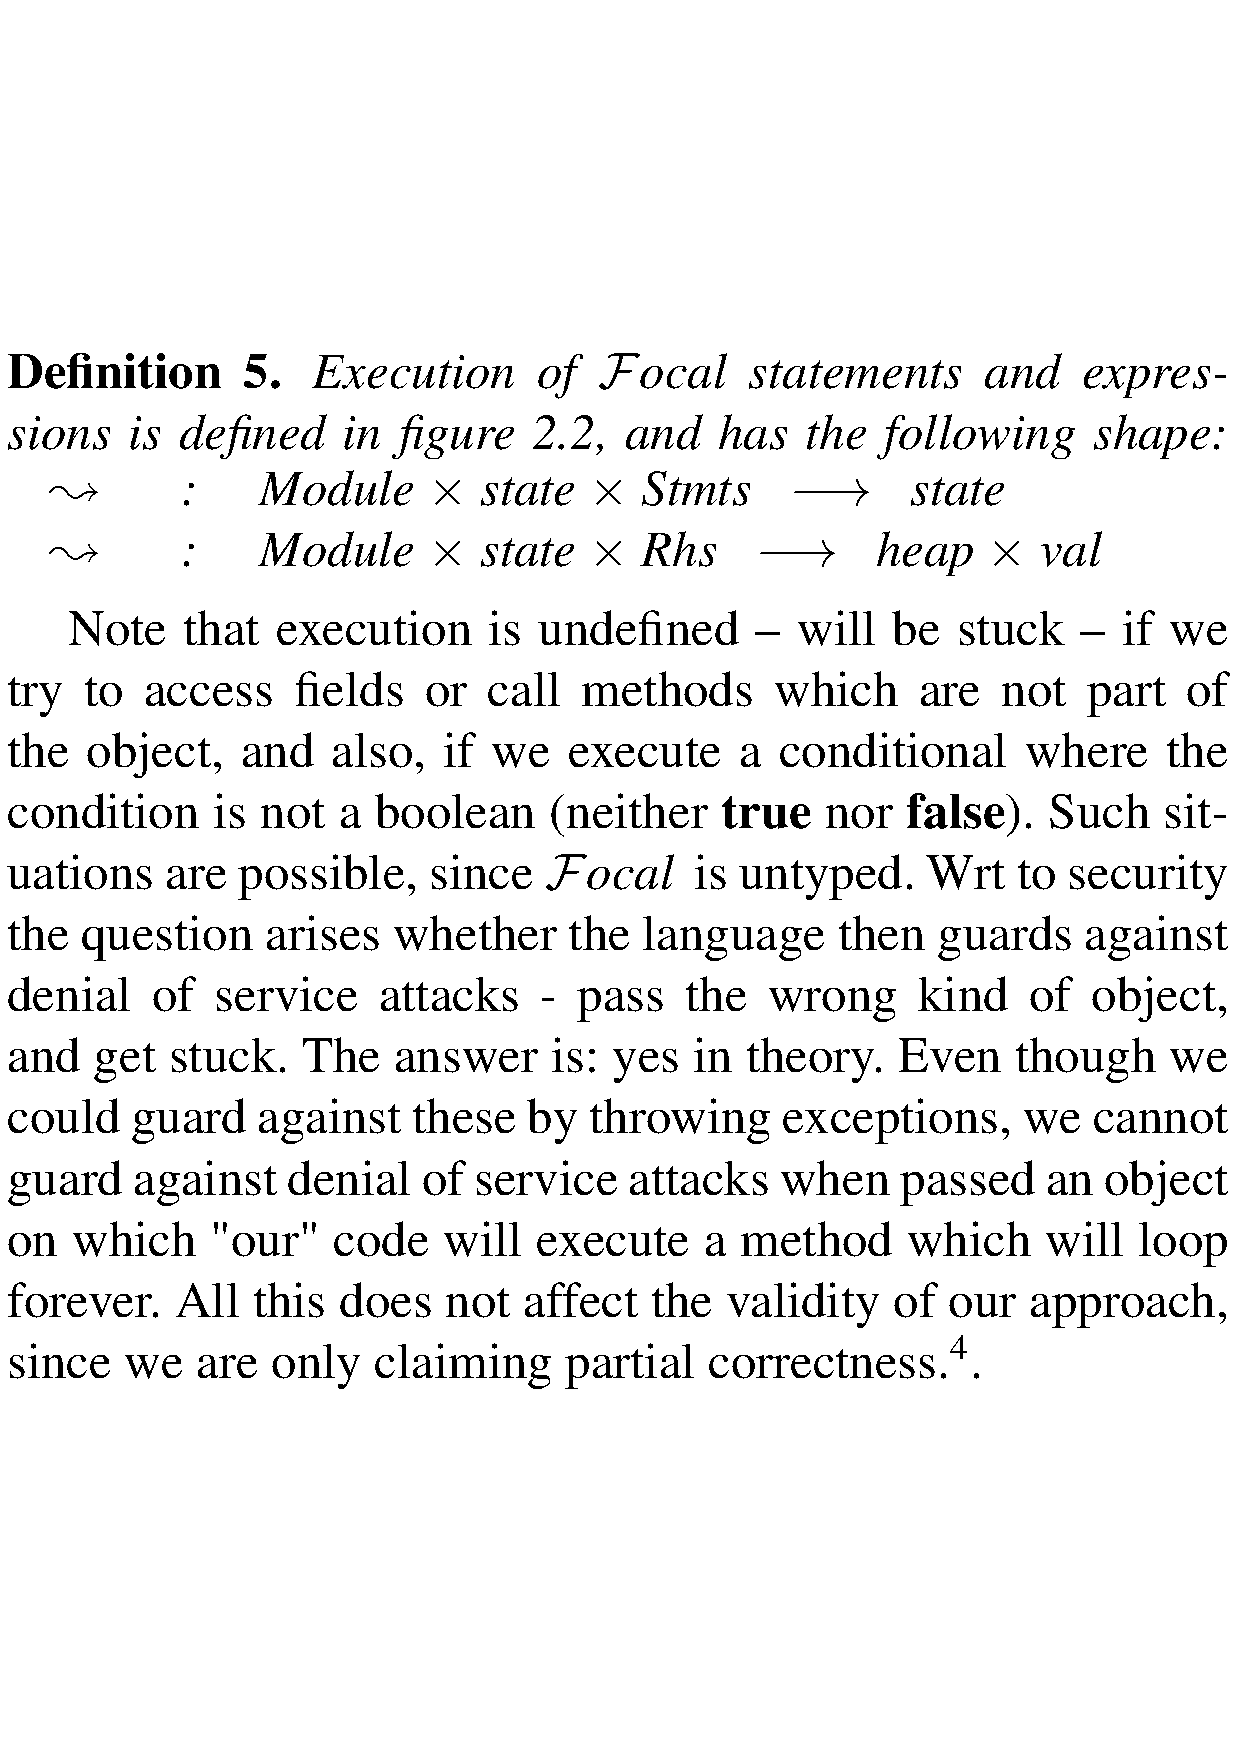
\includegraphics[trim={0 5cm 0 5cm},width=0.5\textwidth]{figures/app_execution.pdf}\linebreak
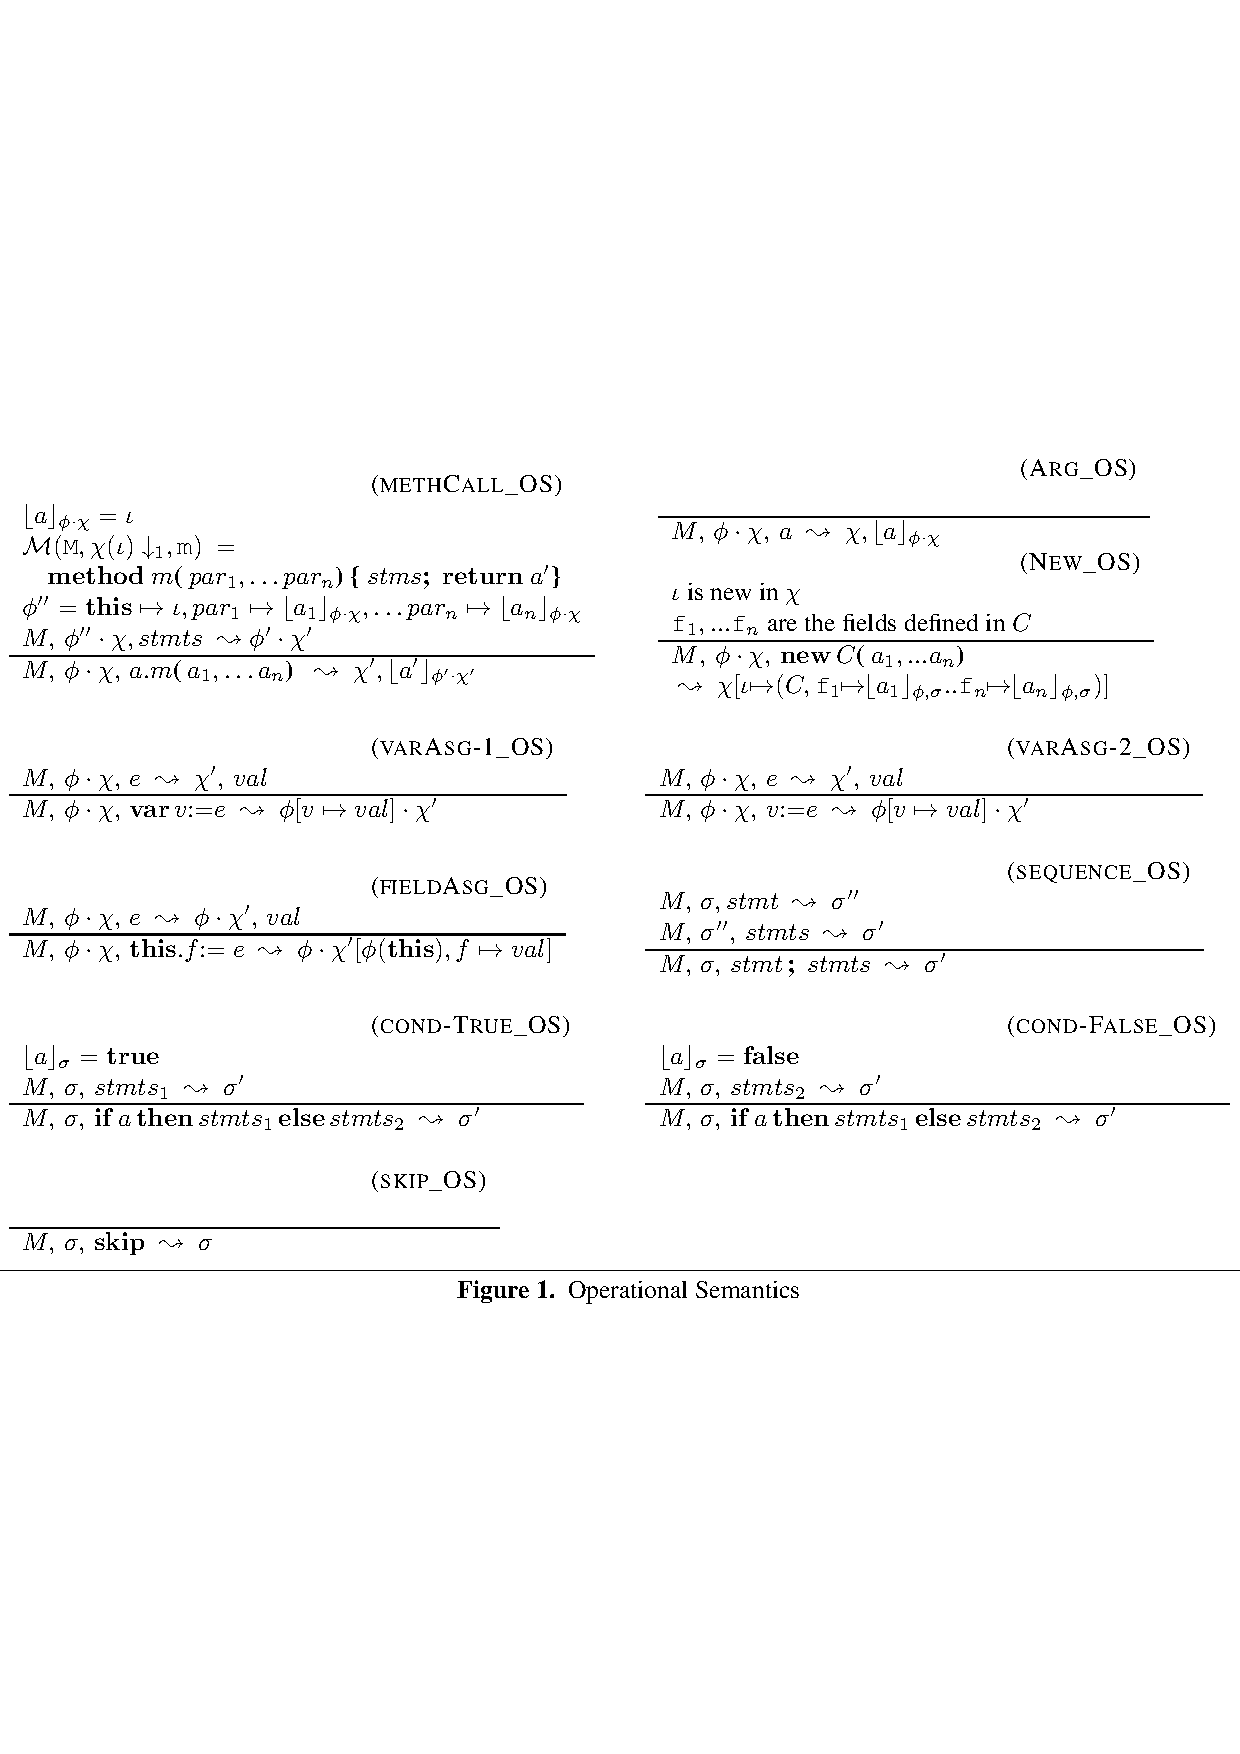
\includegraphics[trim={0 0 0 0cm},width=\textwidth]{figures/app_op.pdf}
\clearpage

\subsubsection{Reach}\label{app:reach}
Here we show the definition of execution and the operational semantics found in the appendix of \cite{drossopoulou2015b}.\\

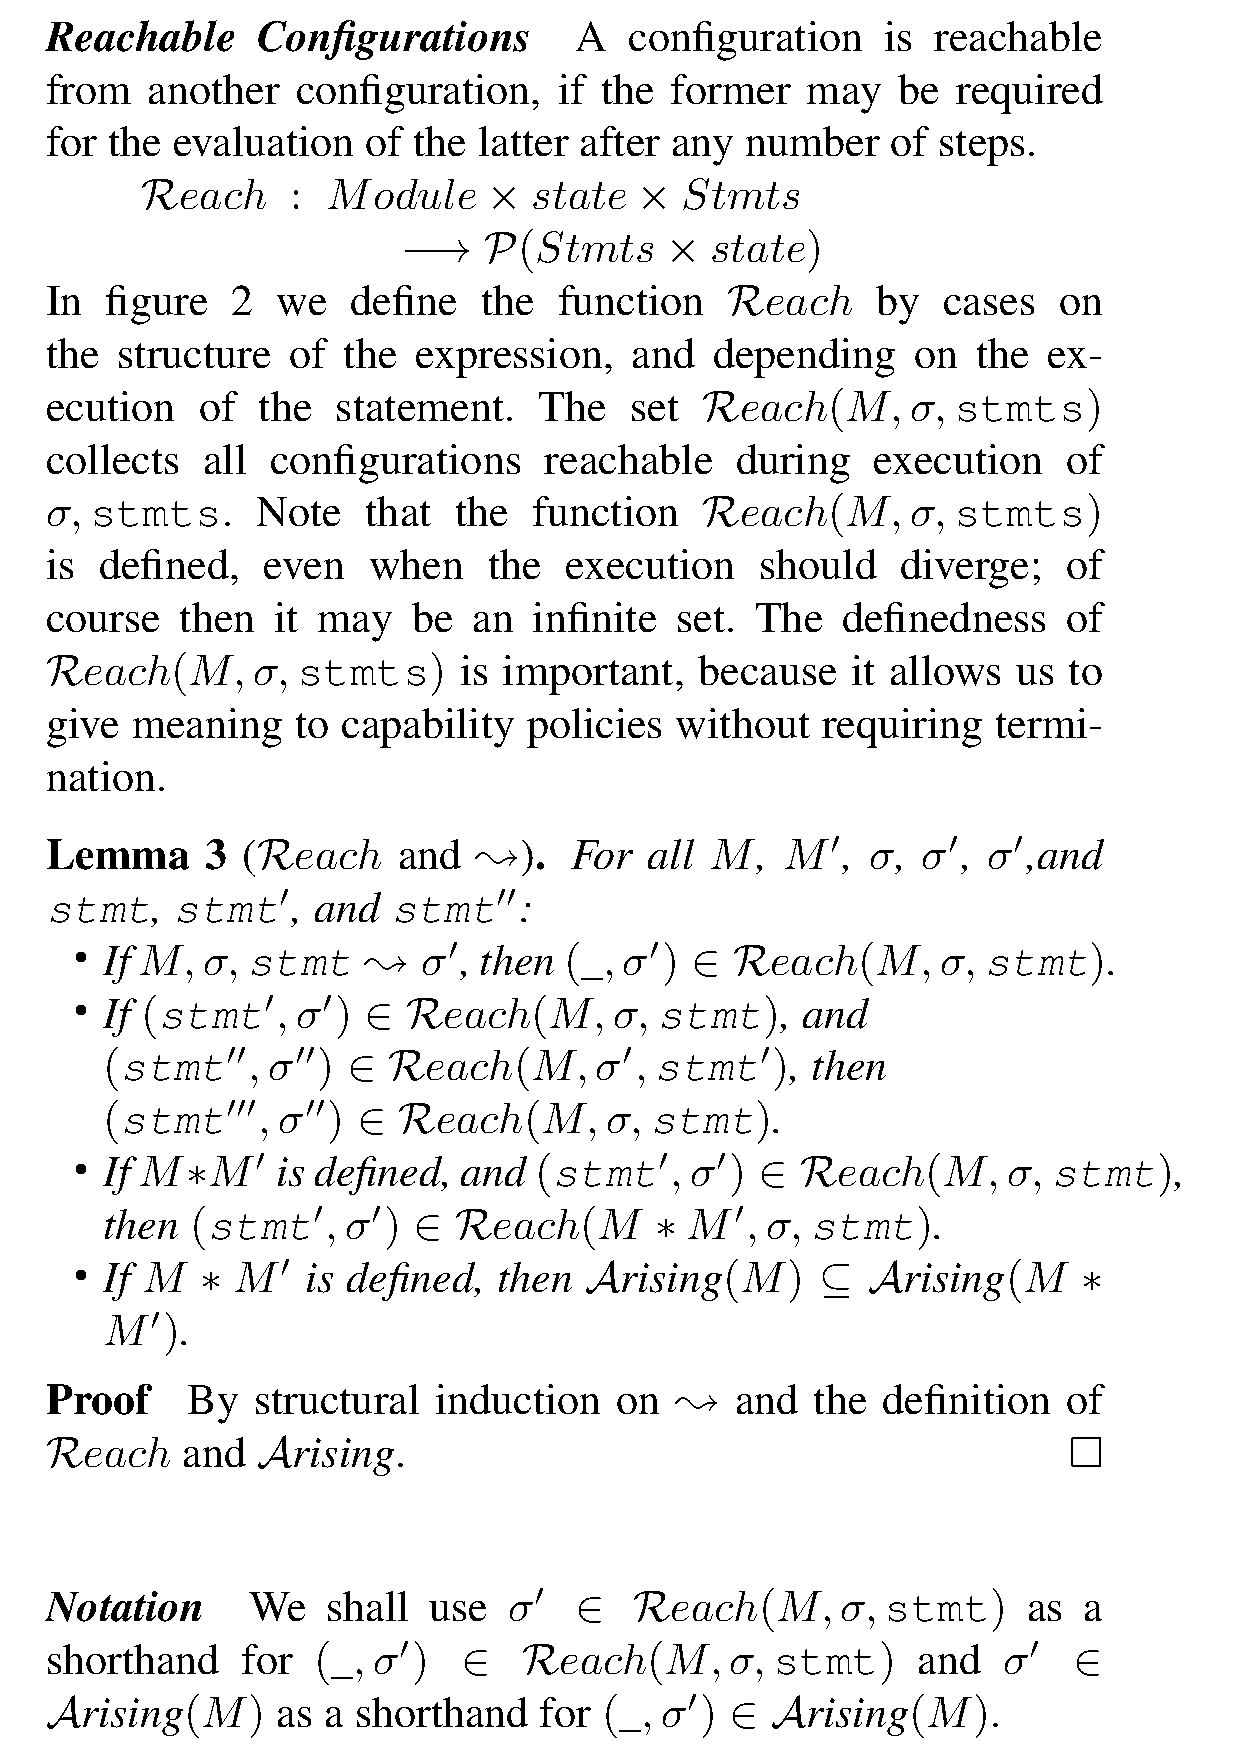
\includegraphics[trim={0 0 0 0},width=0.5\textwidth]{figures/app_reach.pdf}\linebreak
\clearpage
\subsubsection{Assertion}\label{app:assertion}
Here we show the definition of assertion found in the appendix of \cite{drossopoulou2015b}.\\
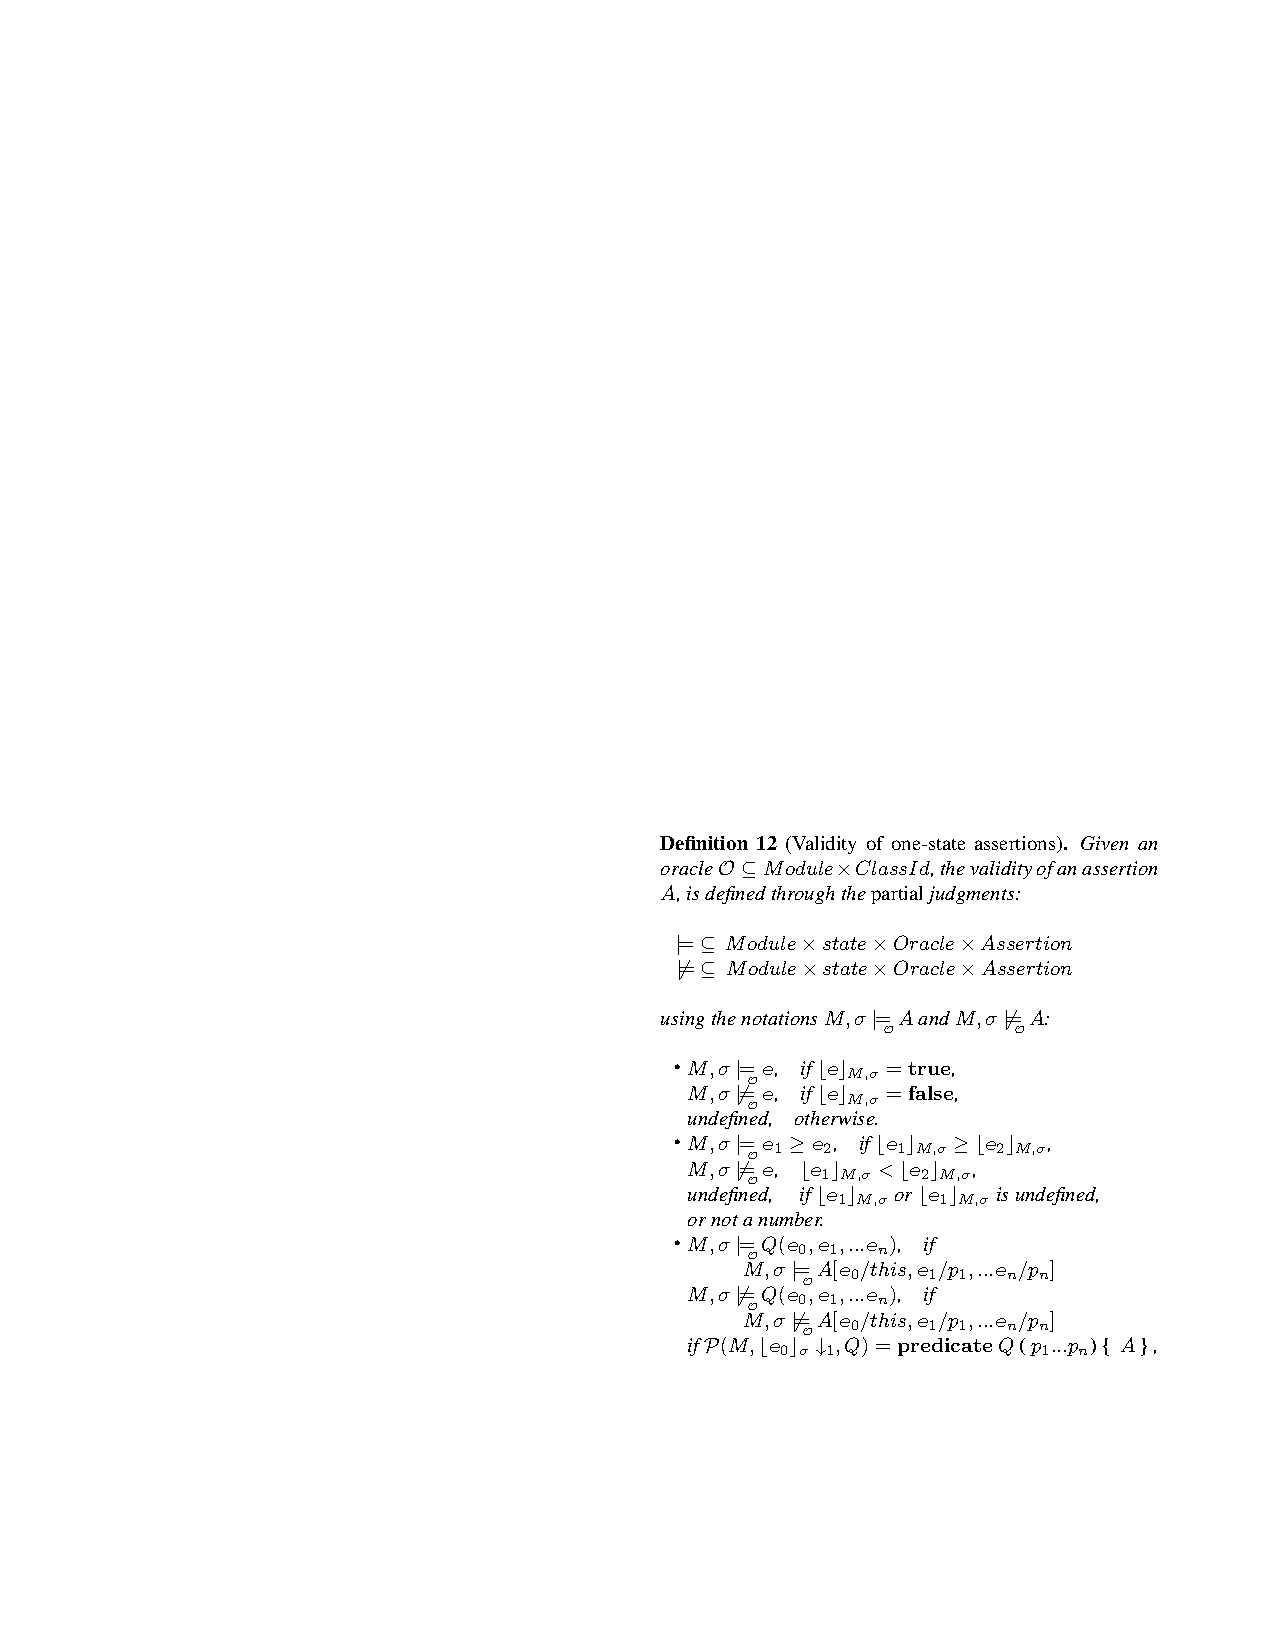
\includegraphics[width=0.5\textwidth,valign=t]{figures/app_assertion1.pdf}
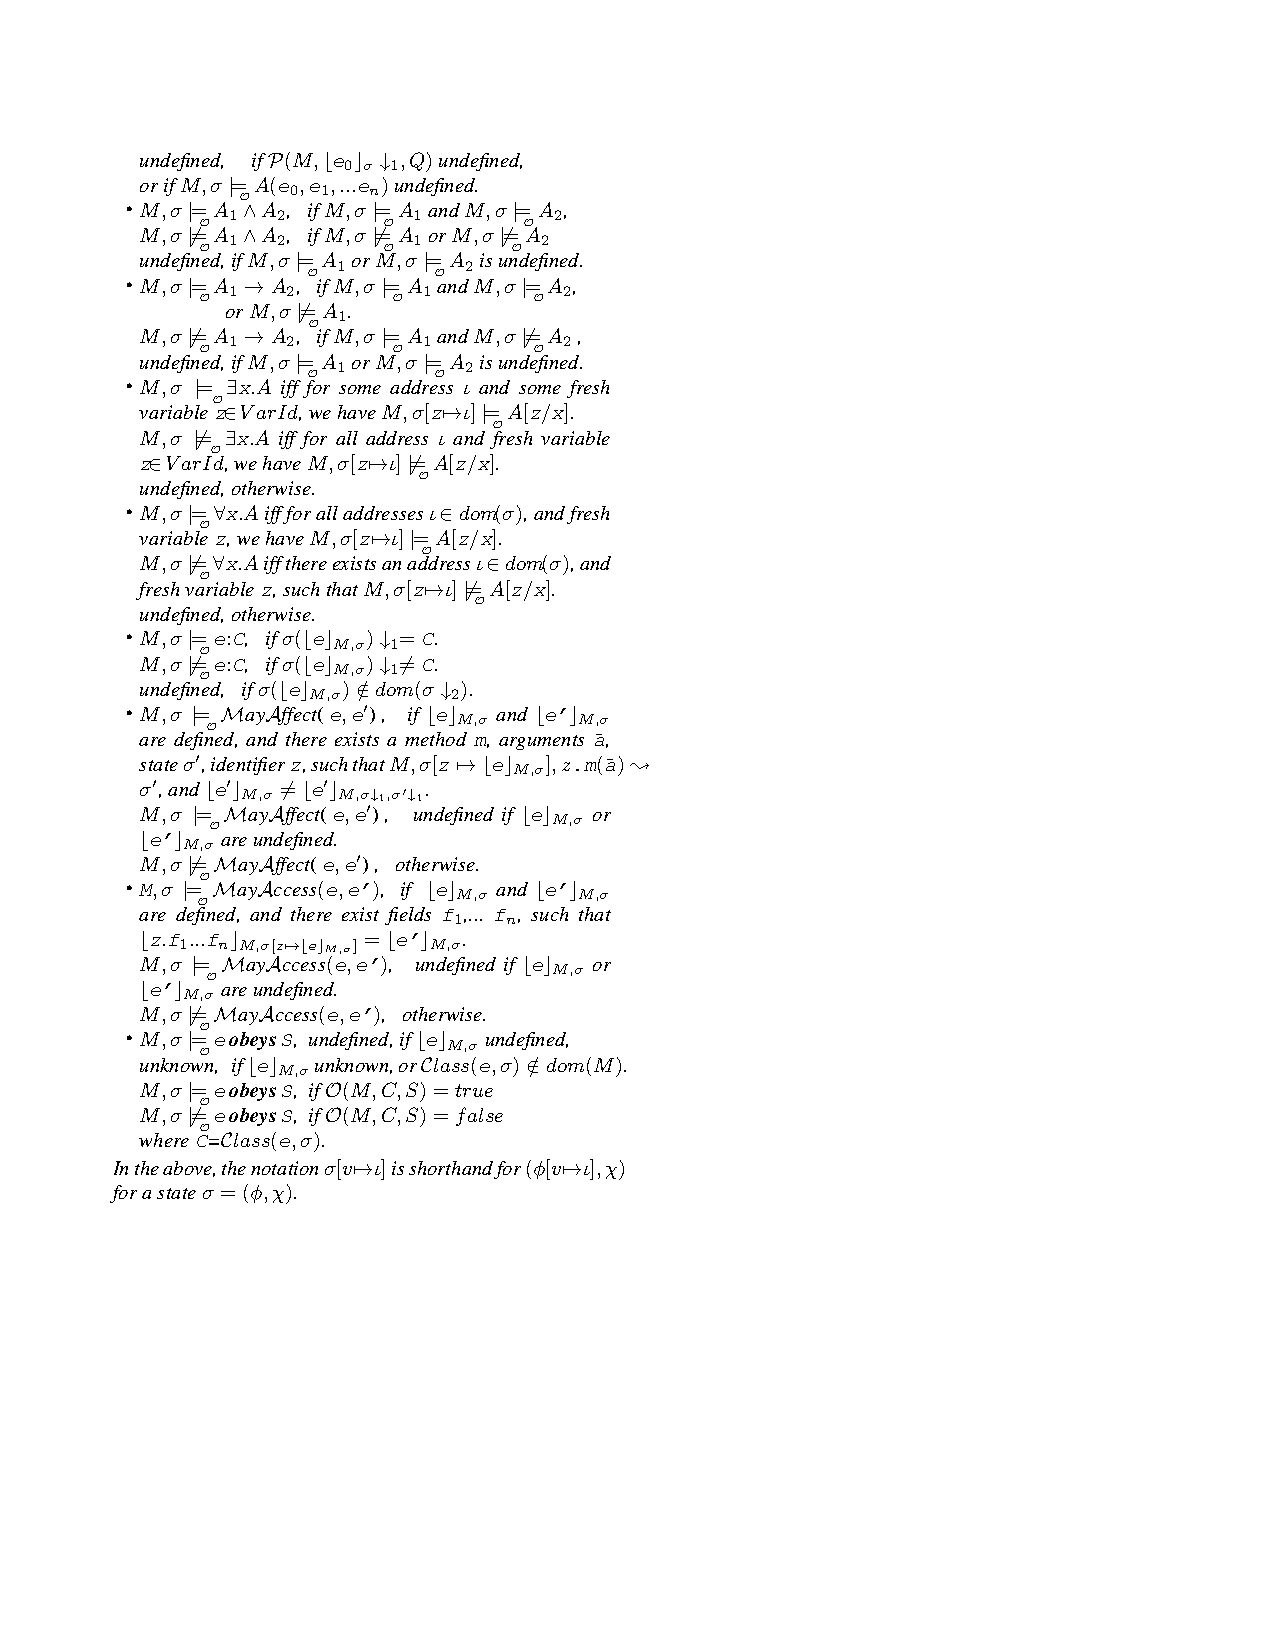
\includegraphics[width=0.5\textwidth,valign=t]{figures/app_assertion2.pdf}
\clearpage
\subsubsection{Module Linking}\label{app:modulelinking}
Here we show the definition of module linking found in the appendix of \cite{drossopoulou2015b}.\\
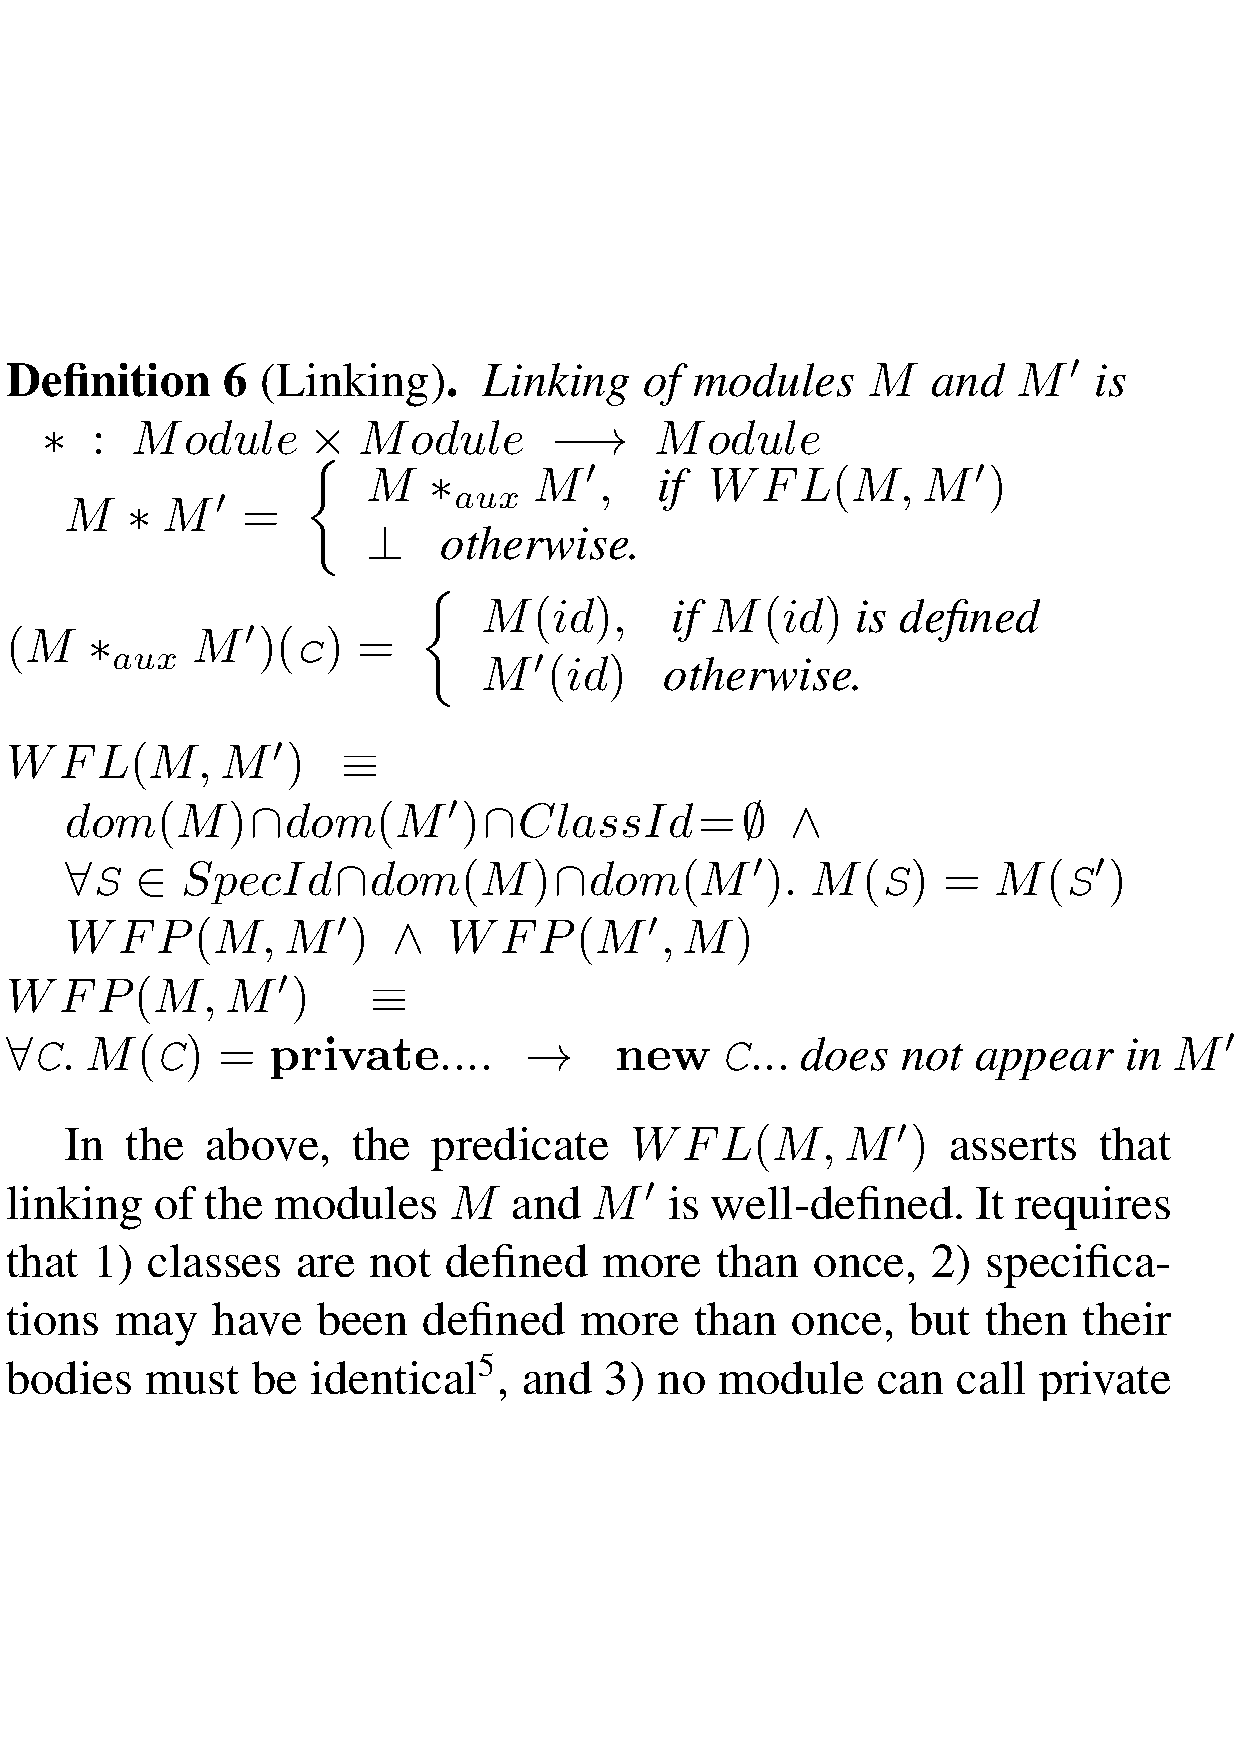
\includegraphics[trim={0 5cm 0 5cm},width=0.5\textwidth,valign=t]{figures/app_modlink1.pdf}\linebreak
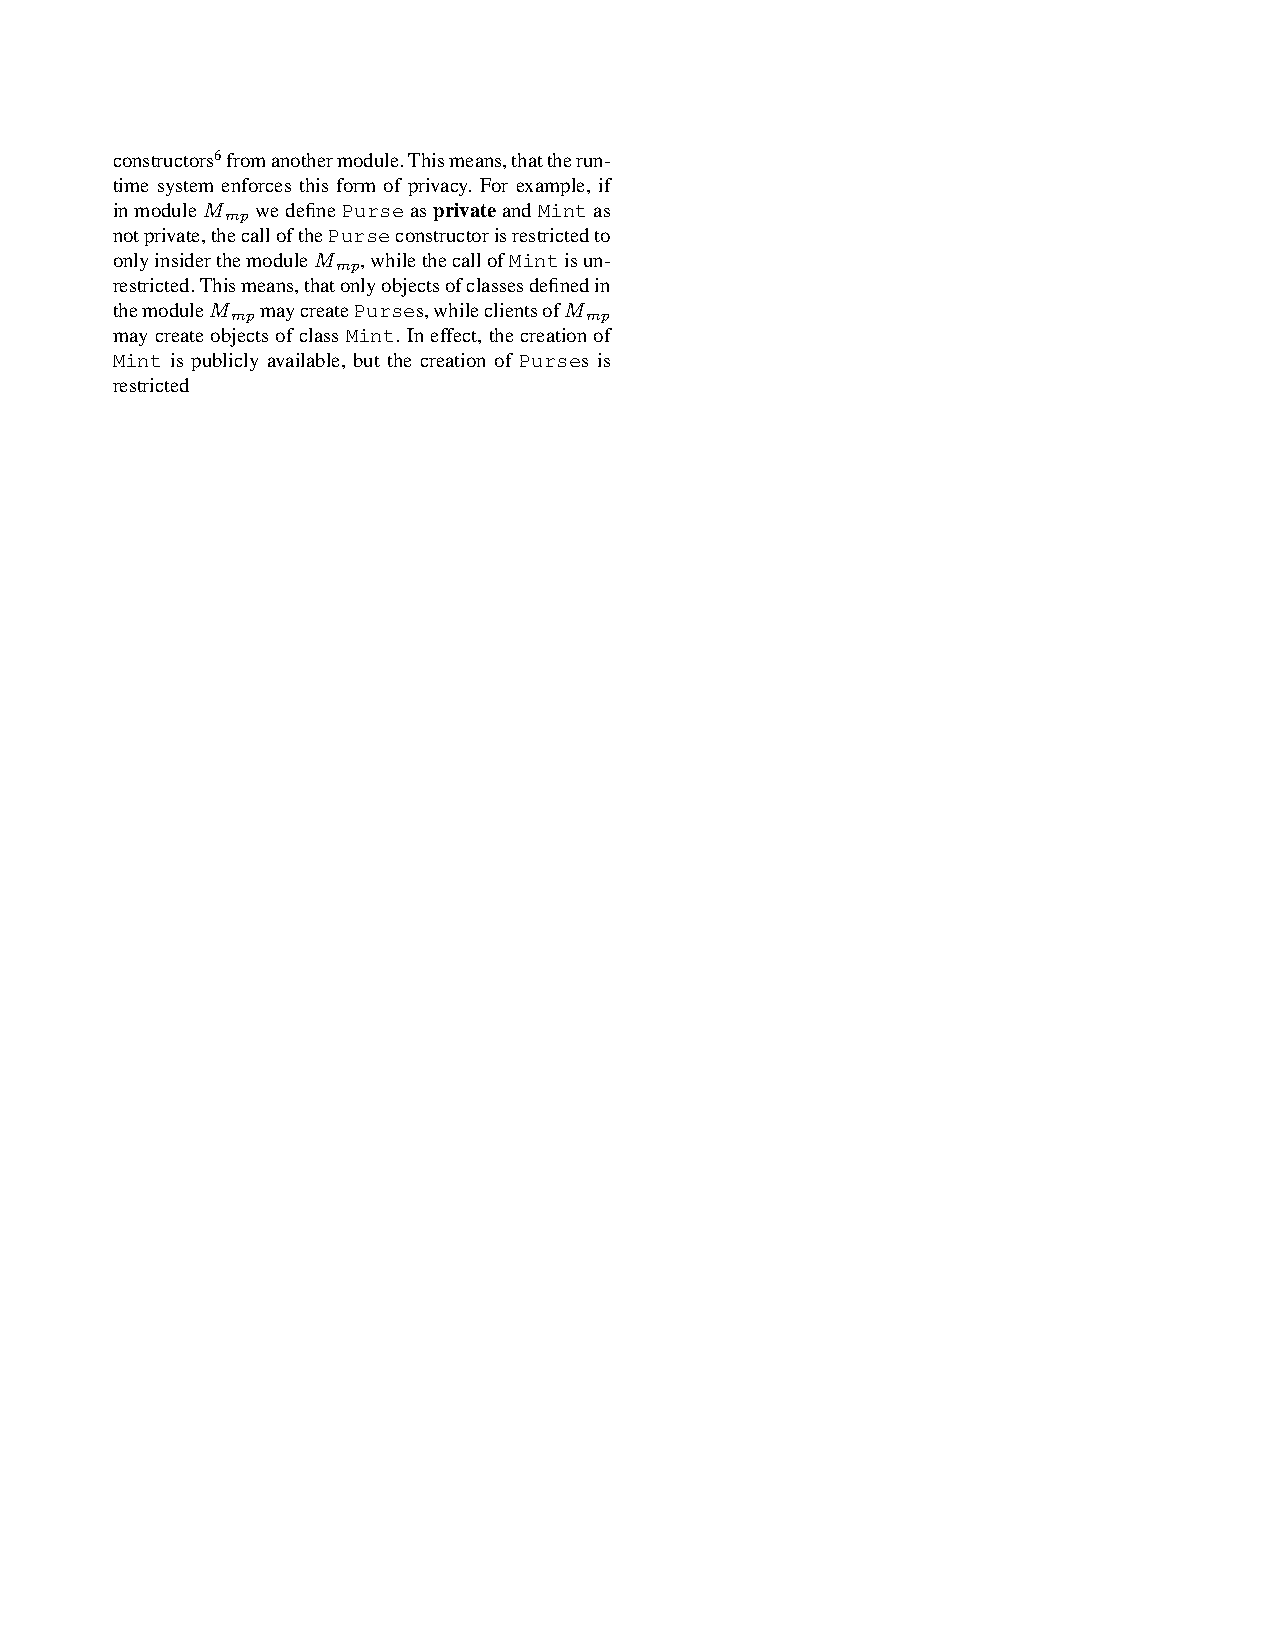
\includegraphics[width=0.5\textwidth,valign=t]{figures/app_modlink2.pdf}
\clearpage
\subsection{Pony Code - DOM Tree}\label{sec:code_DOM}
\begin{minipage}{\textwidth}
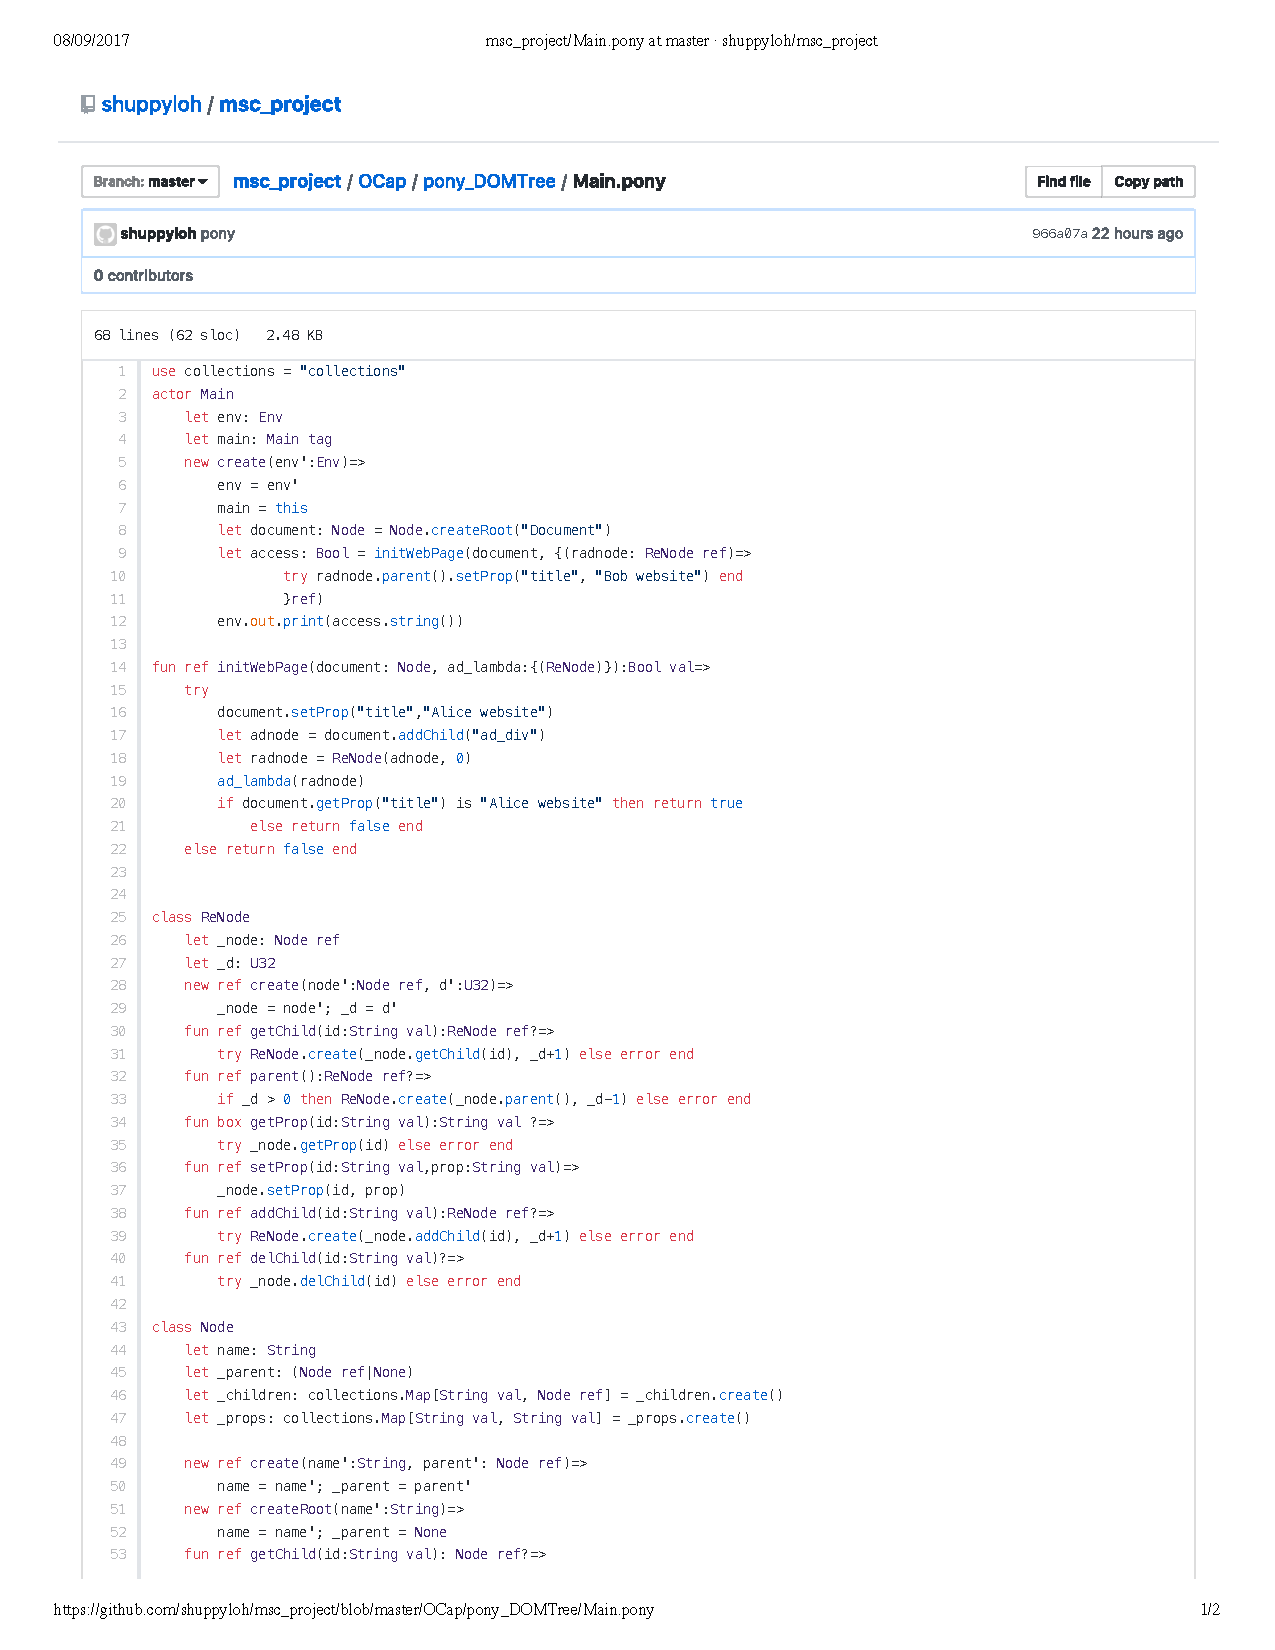
\includegraphics[width=\textwidth,valign=t,page=1]{figures/code_DOM.pdf}
\end{minipage}\clearpage
\begin{minipage}{\textwidth}
\includegraphics[width=\textwidth,valign=t,page=2]{figures/code_DOM.pdf}
\end{minipage}\clearpage
\subsection{Pony Code - Caretaker}\label{sec:code_Caretaker}
\begin{minipage}{\textwidth}
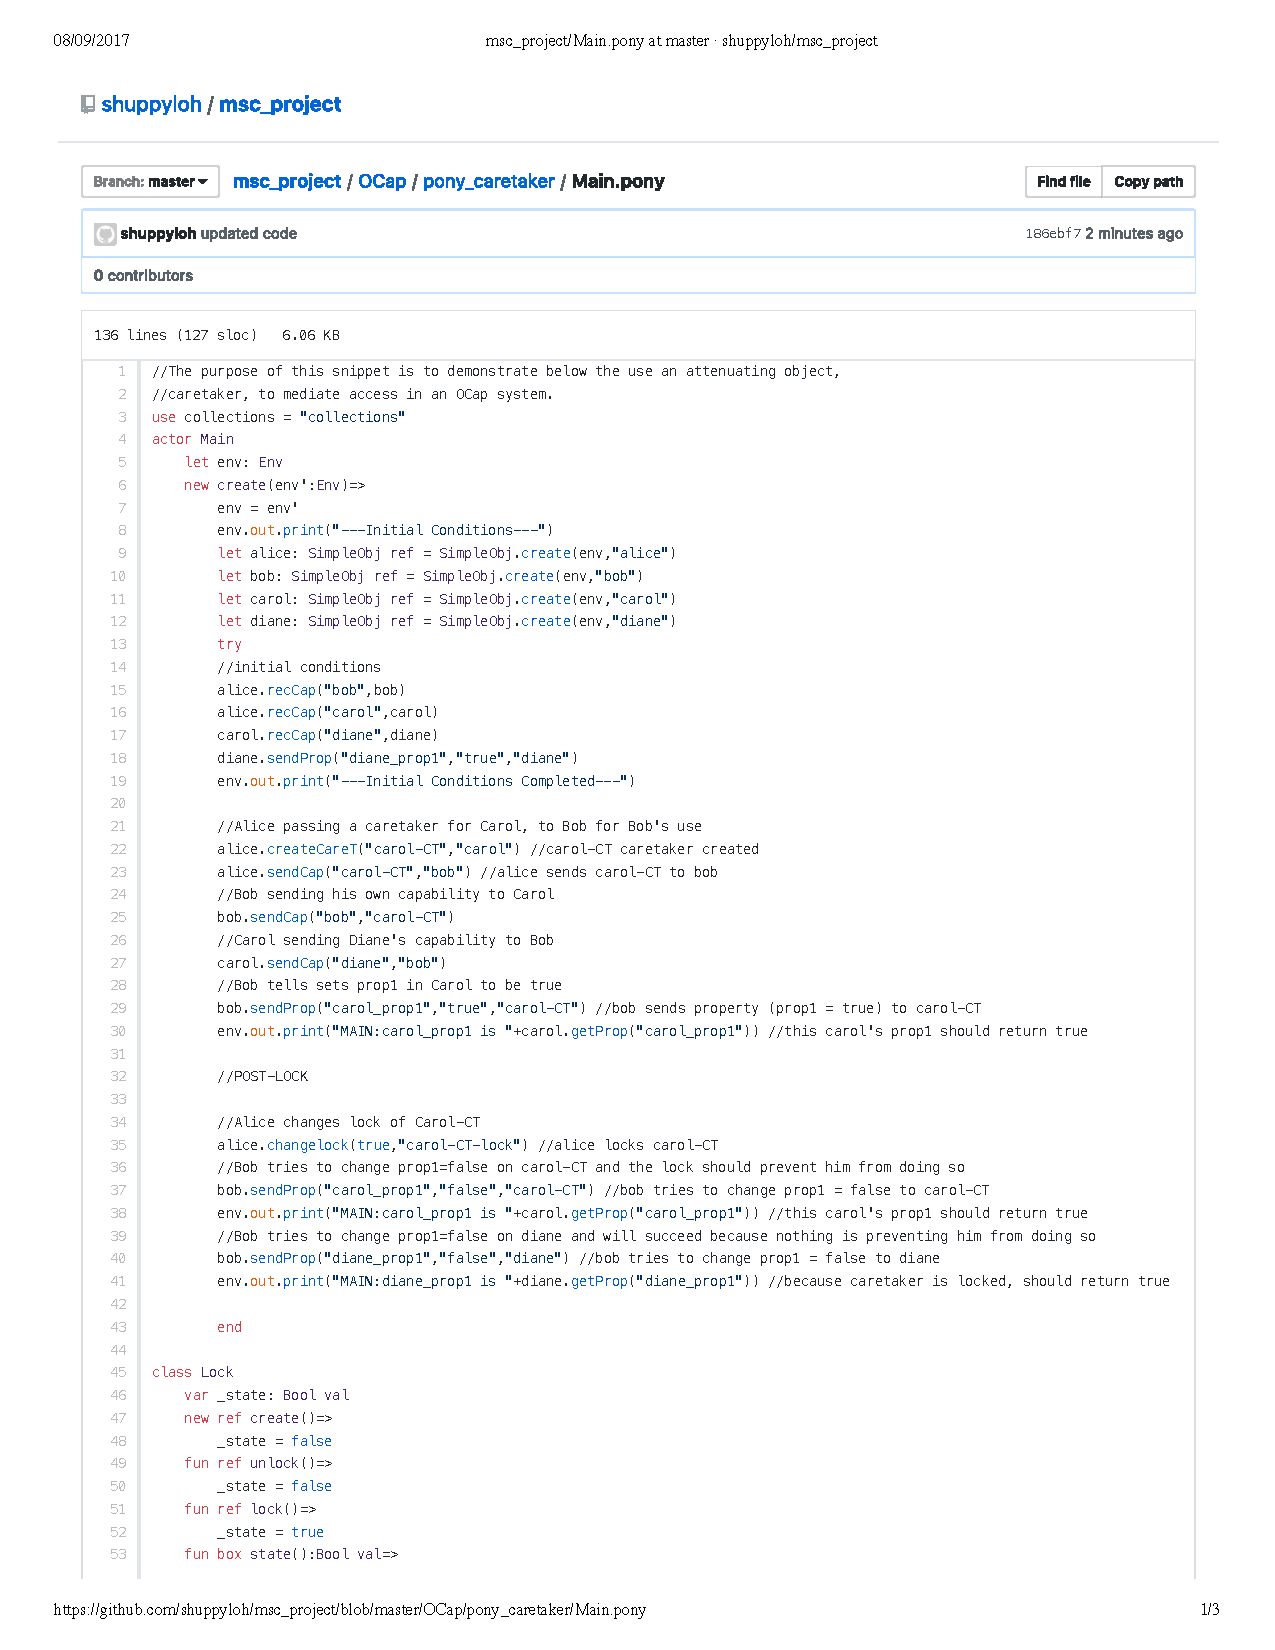
\includegraphics[width=\textwidth,valign=t,page=1]{figures/code_Caretaker.pdf}
\end{minipage}\clearpage
\begin{minipage}{\textwidth}
\includegraphics[width=\textwidth,valign=t,page=2]{figures/code_Caretaker.pdf}
\end{minipage}\clearpage
\begin{minipage}{\textwidth}
\includegraphics[width=\textwidth,valign=t,page=3]{figures/code_Caretaker.pdf}
\end{minipage}\clearpage
\subsection{Pony Code - Membrane}\label{sec:code_Membrane}
\begin{minipage}{\textwidth}
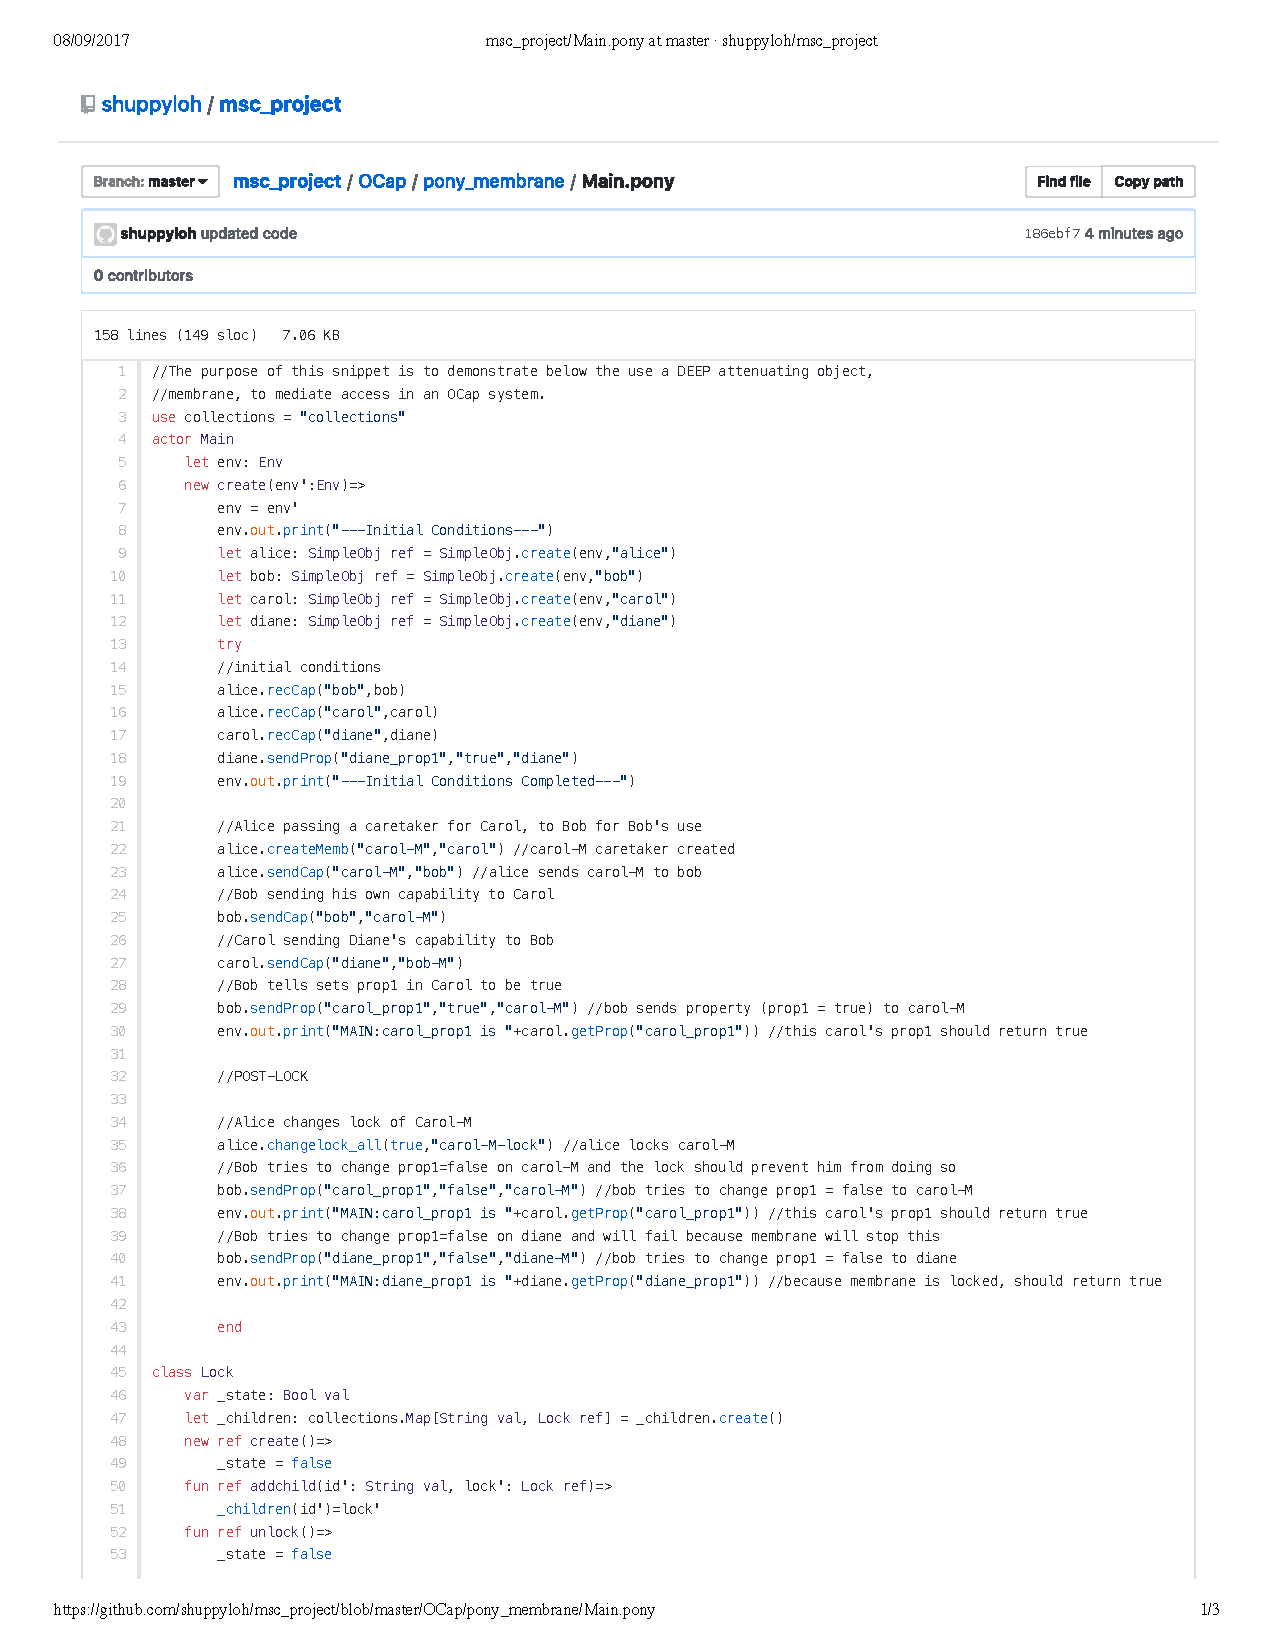
\includegraphics[width=\textwidth,valign=t,page=1]{figures/code_Membrane.pdf}
\end{minipage}\clearpage
\begin{minipage}{\textwidth}
\includegraphics[width=\textwidth,valign=t,page=2]{figures/code_Membrane.pdf}
\end{minipage}\clearpage
\begin{minipage}{\textwidth}
\includegraphics[width=\textwidth,valign=t,page=3]{figures/code_Membrane.pdf}
\end{minipage}\clearpage

%----------------------------------------------------------------------------------------

\end{document}

